\documentclass[11pt,]{article}
\usepackage[left=1in,top=1in,right=1in,bottom=1in]{geometry}
\newcommand*{\authorfont}{\fontfamily{phv}\selectfont}
\usepackage[sc, osf]{mathpazo}


  \usepackage[T1]{fontenc}
  \usepackage[utf8]{inputenc}




\usepackage{abstract}
\renewcommand{\abstractname}{}    % clear the title
\renewcommand{\absnamepos}{empty} % originally center

\renewenvironment{abstract}
 {{%
    \setlength{\leftmargin}{0mm}
    \setlength{\rightmargin}{\leftmargin}%
  }%
  \relax}
 {\endlist}

\makeatletter
\def\@maketitle{%
  \newpage
%  \null
%  \vskip 2em%
%  \begin{center}%
  \let \footnote \thanks
    {\fontsize{18}{20}\selectfont\raggedright  \setlength{\parindent}{0pt} \@title \par}%
}
%\fi
\makeatother


\renewcommand*\thetable{A.\arabic{table}}
\renewcommand*\thefigure{A.\arabic{figure}}


\setcounter{secnumdepth}{0}

\usepackage{longtable,booktabs}

\usepackage{graphicx,grffile}
\makeatletter
\def\maxwidth{\ifdim\Gin@nat@width>\linewidth\linewidth\else\Gin@nat@width\fi}
\def\maxheight{\ifdim\Gin@nat@height>\textheight\textheight\else\Gin@nat@height\fi}
\makeatother
% Scale images if necessary, so that they will not overflow the page
% margins by default, and it is still possible to overwrite the defaults
% using explicit options in \includegraphics[width, height, ...]{}
\setkeys{Gin}{width=\maxwidth,height=\maxheight,keepaspectratio}


\title{The Effect of White Social Prejudice on Support for American Democracy: Supplemental Appendix  }



\author{\Large Steven V. Miller\vspace{0.05in} \newline\normalsize\emph{Clemson University}   \and \Large Nicholas T. Davis\vspace{0.05in} \newline\normalsize\emph{University of Alabama}  }


\date{}

\usepackage{titlesec}

\titleformat*{\section}{\normalsize\bfseries}
\titleformat*{\subsection}{\normalsize\itshape}
\titleformat*{\subsubsection}{\normalsize\itshape}
\titleformat*{\paragraph}{\normalsize\itshape}
\titleformat*{\subparagraph}{\normalsize\itshape}


\usepackage{natbib}
\bibliographystyle{apsr}
\usepackage[strings]{underscore} % protect underscores in most circumstances



\newtheorem{hypothesis}{Hypothesis}
\usepackage{setspace}


% set default figure placement to htbp
\makeatletter
\def\fps@figure{htbp}
\makeatother

\usepackage{array}
\usepackage{caption}
\usepackage{graphicx}
\usepackage{siunitx}
\usepackage[table]{xcolor}
\usepackage{multirow}
\usepackage{hhline}
\usepackage{calc}
\usepackage{tabularx}
\usepackage{fontawesome}
\usepackage[para,online,flushleft]{threeparttable}

% move the hyperref stuff down here, after header-includes, to allow for - \usepackage{hyperref}

\makeatletter
\@ifpackageloaded{hyperref}{}{%
\ifxetex
  \PassOptionsToPackage{hyphens}{url}\usepackage[setpagesize=false, % page size defined by xetex
              unicode=false, % unicode breaks when used with xetex
              xetex]{hyperref}
\else
  \PassOptionsToPackage{hyphens}{url}\usepackage[draft,unicode=true]{hyperref}
\fi
}

\@ifpackageloaded{color}{
    \PassOptionsToPackage{usenames,dvipsnames}{color}
}{%
    \usepackage[usenames,dvipsnames]{color}
}
\makeatother
\hypersetup{breaklinks=true,
            bookmarks=true,
            pdfauthor={Steven V. Miller (Clemson University) and Nicholas T. Davis (University of Alabama)},
             pdfkeywords = {},  
            pdftitle={The Effect of White Social Prejudice on Support for American Democracy: Supplemental Appendix},
            colorlinks=true,
            citecolor=blue,
            urlcolor=blue,
            linkcolor=black,
            pdfborder={0 0 0}}
\urlstyle{same}  % don't use monospace font for urls

% Add an option for endnotes. -----


% add tightlist ----------
\providecommand{\tightlist}{%
\setlength{\itemsep}{0pt}\setlength{\parskip}{0pt}}

% add some other packages ----------

% \usepackage{multicol}
% This should regulate where figures float
% See: https://tex.stackexchange.com/questions/2275/keeping-tables-figures-close-to-where-they-are-mentioned
\usepackage[section]{placeins}


\begin{document}
	
% \pagenumbering{arabic}% resets `page` counter to 1 
%%\renewcommand*{\thepage}{A--\arabic{page}}
%
% \maketitle

{% \usefont{T1}{pnc}{m}{n}
\setlength{\parindent}{0pt}
\thispagestyle{plain}
{\fontsize{18}{20}\selectfont\raggedright 
\maketitle  % title \par  

}

{
   \vskip 13.5pt\relax \normalsize\fontsize{11}{12} 
\textbf{\authorfont Steven V. Miller} \hskip 15pt \emph{\small Clemson University}   \par \textbf{\authorfont Nicholas T. Davis} \hskip 15pt \emph{\small University of Alabama}   

}

}






\vskip -8.5pt

{
\hypersetup{linkcolor=black}
\setcounter{tocdepth}{2}
\tableofcontents
}

 % removetitleabstract

\noindent  

\newpage
\singlespacing

\listoffigures

\listoftables

\newpage

\singlespacing

\hypertarget{introduction}{%
\section{Introduction}\label{introduction}}

This is the supplemental appendix to ``The Effect of White Social
Prejudice on Support for American Democracy'', currently a working paper
in preparation for submission and hopeful acceptance at a peer-reviewed
journal. The supplemental appendix, like the manuscript, is a dynamic
document that automates the code and the presentation of the finished
results in the document itself \citep{xie2013ddrk}. This approach to
document preparation has multiple benefits, namely in the ability to
drive the incidence of transcription error to zero while calling
specific results into the document. We will make some references in this
document to specific statistics that the raw markup will show is a
direct extrapolation from code into presentation. We plan to make the
raw markup available upon request during the peer review process and
will deposit the final analyses to the corresponding author's Github
account upon publication. This will facilitate transparency in published
statistical analysis, consistent with the
\href{http://www.dartstatement.org/}{Data Access and Research
Transparency Initiative} (DA-RT) by the American Political Science
Association.

\hypertarget{descriptive-statistics}{%
\section{Descriptive Statistics}\label{descriptive-statistics}}

We start the supplemental appendix with basic descriptive statistics for
the variables we present in the manuscript. We choose to be brief in
this section of the appendix since this information is descriptive and
provides basic background information about the analyses we present in
the manuscript.

Table \ref{tab:descript} is a basic table of descriptive statistics for
all variables used in Figure 2 in the manuscript, intuitively subsetting
the descriptive statistics to just those Americans in the survey that
self-identify as white. We took care to note that we standardized all
variables by two standard deviations around the mean for all non-binary
inputs, which is consistent with best practice in the mixed effects
modeling framework \citep[c.f.][]{gelman2008sri}. Here, we present the
summary statistics for the raw inputs and, for ease, do not present
summary statistics for the square terms we also derive from the age and
ideology variables.

\begin{table}[!h]

\caption{\label{tab:descript}Descriptive Statistics for Variables Used in Figure 2 in the Manuscript}
\centering
\resizebox{\linewidth}{!}{
\begin{tabular}{lcccccccc}
\toprule
\textbf{Variable} & \textbf{Mean} & \textbf{S.D.} & \textbf{Min.} & \textbf{Median} & \textbf{Max.} & \textbf{N} & \textbf{Total N} & \textbf{Perc. Valid}\\
\midrule
Age & 48.922 & 17.245 & 18.000 & 48.500 & 94.000 & 4606 & 4621 & 99.7\%\\
Army Rule (Dummy) & 0.425 & 0.494 & 0.000 & 0.000 & 1.000 & 4476 & 4621 & 96.9\%\\
College Educated & 0.295 & 0.456 & 0.000 & 0.000 & 1.000 & 4621 & 4621 & 100\%\\
Democrat & 0.411 & 0.492 & 0.000 & 0.000 & 1.000 & 3838 & 4621 & 83.1\%\\
Female & 0.524 & 0.499 & 0.000 & 1.000 & 1.000 & 4621 & 4621 & 100\%\\
\addlinespace
Republican & 0.446 & 0.497 & 0.000 & 0.000 & 1.000 & 3838 & 4621 & 83.1\%\\
Oppose Democracy (Dummy) & 0.123 & 0.329 & 0.000 & 0.000 & 1.000 & 4454 & 4621 & 96.4\%\\
Ideology & 4.811 & 1.958 & 0.000 & 4.000 & 9.000 & 4394 & 4621 & 95.1\%\\
Income Scale & 4.652 & 2.267 & 0.000 & 5.000 & 9.000 & 4344 & 4621 & 94\%\\
Emancipative Values & 0.003 & 0.488 & -1.499 & -0.036 & 1.341 & 4621 & 4621 & 100\%\\
\addlinespace
Strong Leader (Dummy) & 0.249 & 0.433 & 0.000 & 0.000 & 1.000 & 4505 & 4621 & 97.5\%\\
Unmployed & 0.049 & 0.216 & 0.000 & 0.000 & 1.000 & 4564 & 4621 & 98.8\%\\
White Social Prejudice & 0.187 & 0.390 & 0.000 & 0.000 & 1.000 & 4621 & 4621 & 100\%\\
\bottomrule
\end{tabular}}
\end{table}

Figure \ref{fig:barraceyear} provides a quick visual summary of the
variation of number observations by survey wave/year and race/ethnicity.
These categories are obviously not mutually exclusive, nor related in a
meaningful way. We offer this visualization to quickly communicate that
75\% of the third, fourth, fifth, and sixth waves of WVS data featured
respondents who self-identify as white and that the total number of
observations by the survey year for those who self-identify as white.

\begin{figure}
\centering
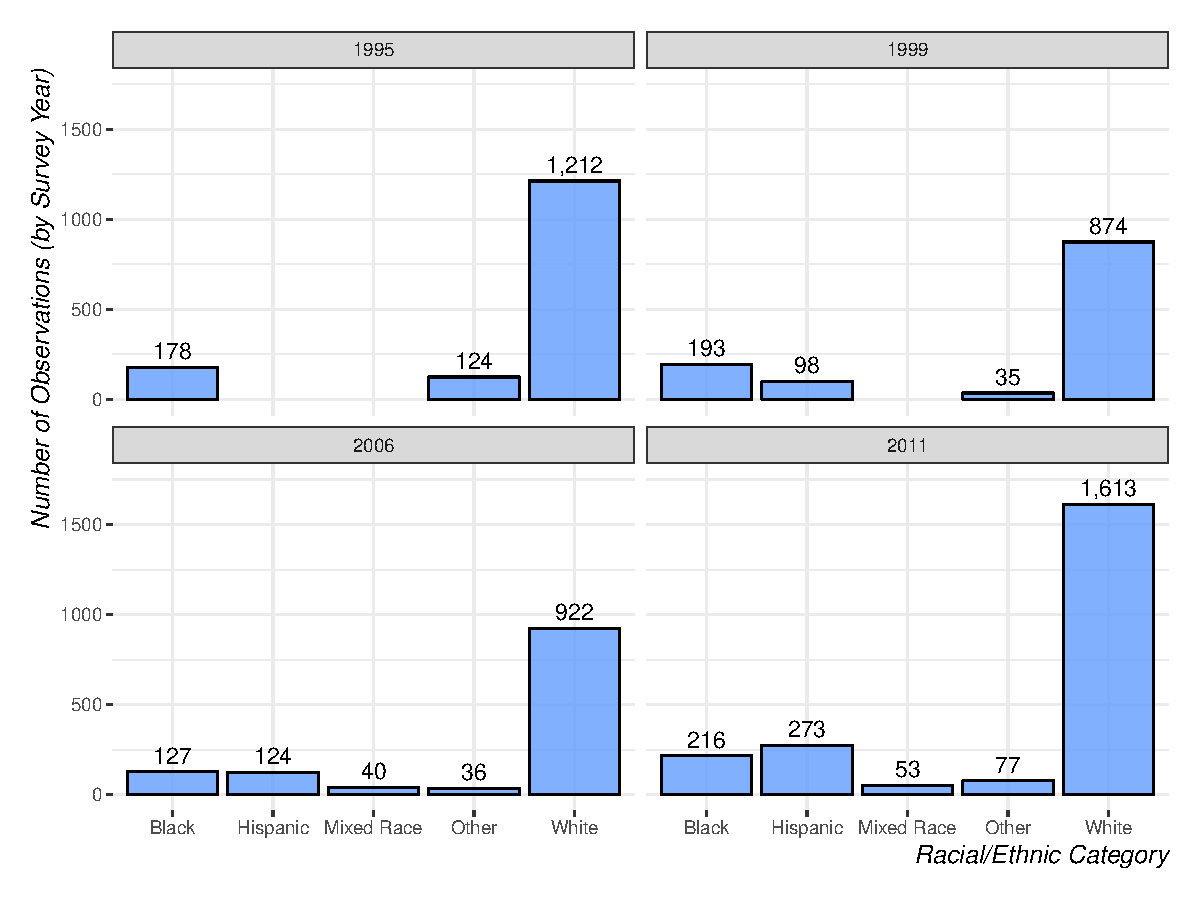
\includegraphics{figs/barraceyear.pdf}
\caption{\label{fig:barraceyear}Number of Observations by Race/Ethnicity
and Survey Year in Our Analyses}
\end{figure}

Figure \ref{fig:corr} provides a correlation matrix of the variables
used in Figure 2 in the analysis. Only two of the covariates show any
meaningful correlation: the dummy for Republican and the dummy for
Democrat. This much is unsurprising since those two variables are
mutually exclusive and serve as fixed effects communicating the effect
of self-identifying with one of the two major parties in the U.S.
relative to the baseline of self-identified independents and third-party
supporters. No two other variables correlate in any meanginful way that
would serve as an estimation problem in the models we report in the
manuscript.

\begin{figure}
\centering
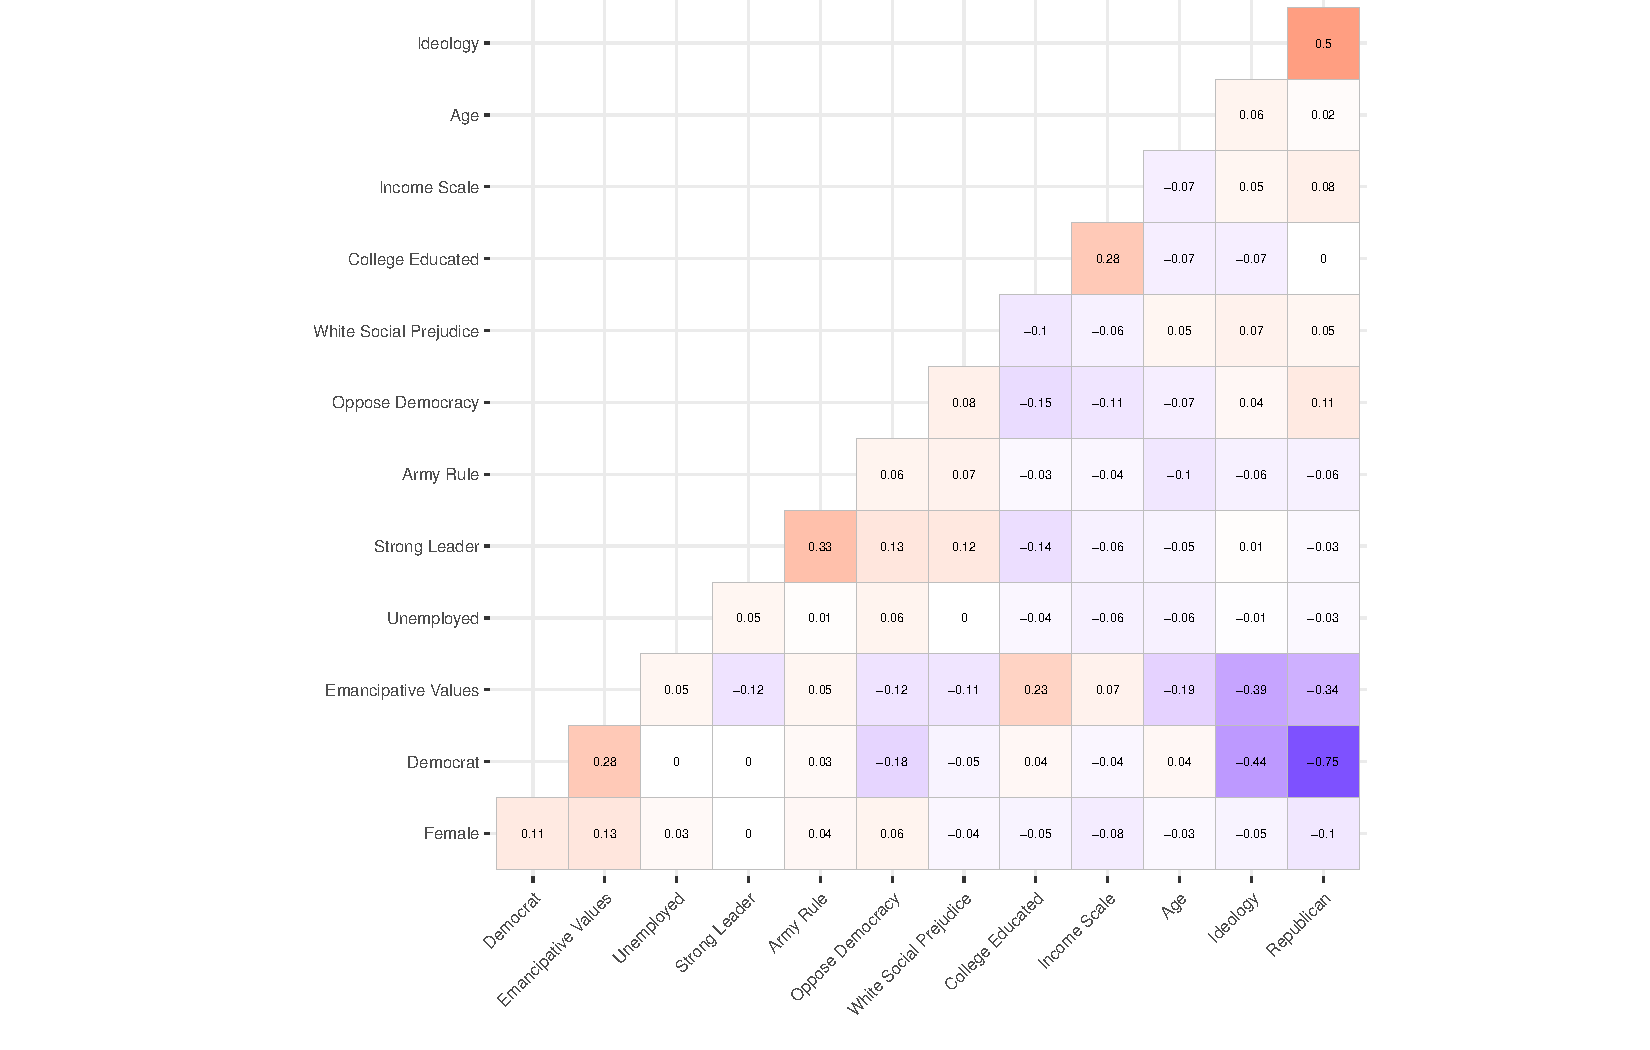
\includegraphics{figs/corr.pdf}
\caption{\label{fig:corr}A Correlation Matrix of the Variables Used in
the Analysis}
\end{figure}

\hypertarget{the-nexus-between-education-and-prejudice}{%
\section{The Nexus Between Education and
Prejudice}\label{the-nexus-between-education-and-prejudice}}

We offer a special section of our analysis to an exploration of the
multifaceted relationship between education and prejudice and support
for democracy. We do this for a few reasons. One, scholarship identifies
that education is a substantively important correlate for both democracy
and tolerance. Some of the earliest scholarship on the topic classified
an educated citizenry as sine qua non feature for democracy to flourish,
bolstering its importance by identifying formal education as a necessary
condition for democracy itself \citep{dewey1916de, lipset1959ssr}. More
recent analyses on the determinants of democracy have largely bolstered
this assertion that education is an important determinant of democracy
and the public demand for more democracy
\citep[e.g.][]{barro1999dd, sanbornthyne2014ld}. These arguments
invariably draw in scholarship that highlights how education socializes
young people. Education involves rote book-learning but also lowers the
cost of some social interactions \citep{glaeseretal2007wddn}, promotes
good citizenship by emphasizing involvement and participatory behavior
\citep{glaeseretal2007wddn, holmes1979iges} and teaches people how to
acquire knowledge through reasoned and peaceable debate
\citep{bowlesgintis1976sca}. In essence, education also promotes
tolerance and tolerance also promotes democracy. Conventional wisdom
holds that all three are mutually reinforcing.

Questions remain about this conventional wisdom in light of current
events and more recent scholarship. For example, increasing education
may lower social prejudice toward ethnic/racial minorities, as the main
results in the manuscript show, but it coincides with an increasing
political prejudice \citep{henrynapier2017ergi} that is
\emph{symmetrical} across the political left and political right. It
suggests a form of selection because increasing education is itself a
form of selection. Individuals often self-select into more education,
and increasing educational attainment, especially at the collegiate
level, may do well to socialize most students about the importance of
democracy, equal opportunity of access for majorities and minorities
within a democratic design, and how to accept the presence of
ethnic/racial outgroups as co-equals. However, students who still hold
those views after selecting into advanced levels of education should be
more likely to have a firm grasp on the ``undesirable''
equality-building features of democracy. This would square with some of
Federico's
\citetext{\citeyear{federico2005rper}; \citeyear{federico2006reir}}
research that finds negative racial perceptions decrease with more
education but the effect of these same negative racial perceptions tends
to be stronger among the better educated. It would also match what we
observed in Charlottesville in 2017, where a ``Unite the Right'' rally
inspired by Richard Spencer (a two-time college graduate) attracted a
significant number of college students who still appeared to hold these
views even after exposure to college-level instruction. In other words,
the effect of holding onto prejudiced views after higher levels of
education may make social prejudice's effect on attitudes against
democracy even stronger even if we typically assume these effects
cluster on the less educated.

We explore this nexus between education and prejudice with two different
estimations of our main analyses. The first alternate estimation allows
the effect of college education and white social prejudice to interact.
The second alternate estimation drops the college education variable but
treats education as a category, or ``random effect'', by which the slope
of white social prejudice can vary. We present the important results
from these models as Figure \ref{fig:interplot} and Figure
\ref{fig:randomslopesplot}.

\begin{figure}
\centering

\includegraphics{figs/educ_interactplot.pdf}
\caption{\label{fig:interplot}Regression Results (a) and Simulated
Probabilities (b) of the Interaction Between College Education and
Prejudice on Anti-Democratic Orientations}
\end{figure}

Figure \ref{fig:interplot} contains two components. The top component is
an abbreviated dot-and-whisker plot that shows just the effect of
college education, white social prejudice, and its interaction, noting
that the other covariates in the model are estimated but ultimately put
in the appendix to draw the reader's attention to the main covariates of
interest. The bottom component is a ridgeline plot of simulated
probabilities of the likelihood of observing a 1 in the model by
different categories of college education and white social prejudice. We
annotate the top right of each ridge with 95\% confidence intervals
surrounding the expected value (i.e.~mean probability) from the
simulations.

We note that the dot-and-whisker plot does show one important difference
between the main results we presented in the manuscript. Namely,
allowing college education to interact with the white social prejudice
measure creates a statistically significant effect on support for army
rule for the constituent term of college education that we did not
observe in the main results we provide in the manuscript. Formally, it
communicates that the effect of increasing college education on those
for whom our white social prejudice measure is zero decreases the
likelihood of thinking rule of government by the army would be good for
the United States. However, the interaction is statistically
insignificant by conventional thresholds. Indeed, only one interactive
effect has an effect that can we discern from zero. The interaction
between college education and white social prejudice is positive and
discernible from zero in the model that explores the outright opposition
to having a democracy for the United States.

The thousand simulations we run for each of these three analyses yields
some interesting findings. Namely, they offer some illustrative evidence
that the effect of white social prejudice on anti-democratic
orientations may be higher on those with more education than those with
less education. Ultimately, the simulations we run show a lot of overlap
among the two-by-two matrix connecting college education and white
social prejudice to attitudes in support of a military government for
the United States. Generally, white social prejudice has a somewhat
large, positive effect on the likelihood of thinking a military
government for the United States is good even though the 95\% intervals
surrounding the mean of the estimations clearly overlap. However, our
simulations suggest that the effect of white social prejudice seems to
be larger on the college-educated.

We see additional evidence suggesting this divergent effect of white
social prejudice by level of education in the models simulating the
likelihood of opposing democracy and thinking strongman rule would be
good for the United States. Here, the bottom two ridges
(i.e.~simulations for the college-educated) show much starker effects of
white social prejudice on the college-educated than on those who did not
complete a college degree. The 95\% intervals barely overlap, for which
we will note that we are not making an inferential statement here, but
the movement we see serves as another noisy signal that the effect of
white social prejudice may be higher on the college-educated than on
those without at least a four-year university degree. Indeed, the
simulations put the college-educated, but prejudiced, white Americans
closer to those non-prejudiced white Americans without a college degree.
Whereas we commonly assume that a university education opens up minds to
appreciate democracy and the importance of broadly enfranchising
citizens to participate in matters of governance, the effect of
prejudice towards immigrants/foreign workers, people of a different
race, and those who speak a different language seems to negate that
effect.

Figure \ref{fig:randomslopesplot} offers further evidence that the
effect of white social prejudice may actually be stronger at higher
levels of education. Here, we re-estimate the three main models from the
main results in the appendix, but drop the college education fixed
effect and substitute instead education categories as random effects.
These education random effect categories are for those respondents
without formal education or did not complete primary education, those
who stopped their education after primary school, those who did not
finish high school/secondary education, high school grads that never
went to college, those that went to college but did not complete a
four-year degree, those with a bachelors or equivalent four-year degree,
and those with an advanced university degree (e.g.~J.D., Ph.D., M.D.,
etc.).\footnote{The ``Some College, No Four-Year Degree'' category
  includes respondents with a traditional two-year associates degree.}
This estimation allows the slope of the fixed effect of white social
prejudice to vary by these levels of the random effect. After estimating
these three models, we ran a thousand simulations on each, calculating
expected values of the likelihood of an anti-democratic orientation
while allowing the white social prejudice fixed effect to vary from 0 to
1 at each level. We report the results of these simulations as expected
values (i.e.~mean probabilities of an anti-democratic orientation in our
simulations) with 95\% intervals at each level of education.

\begin{figure}
\centering
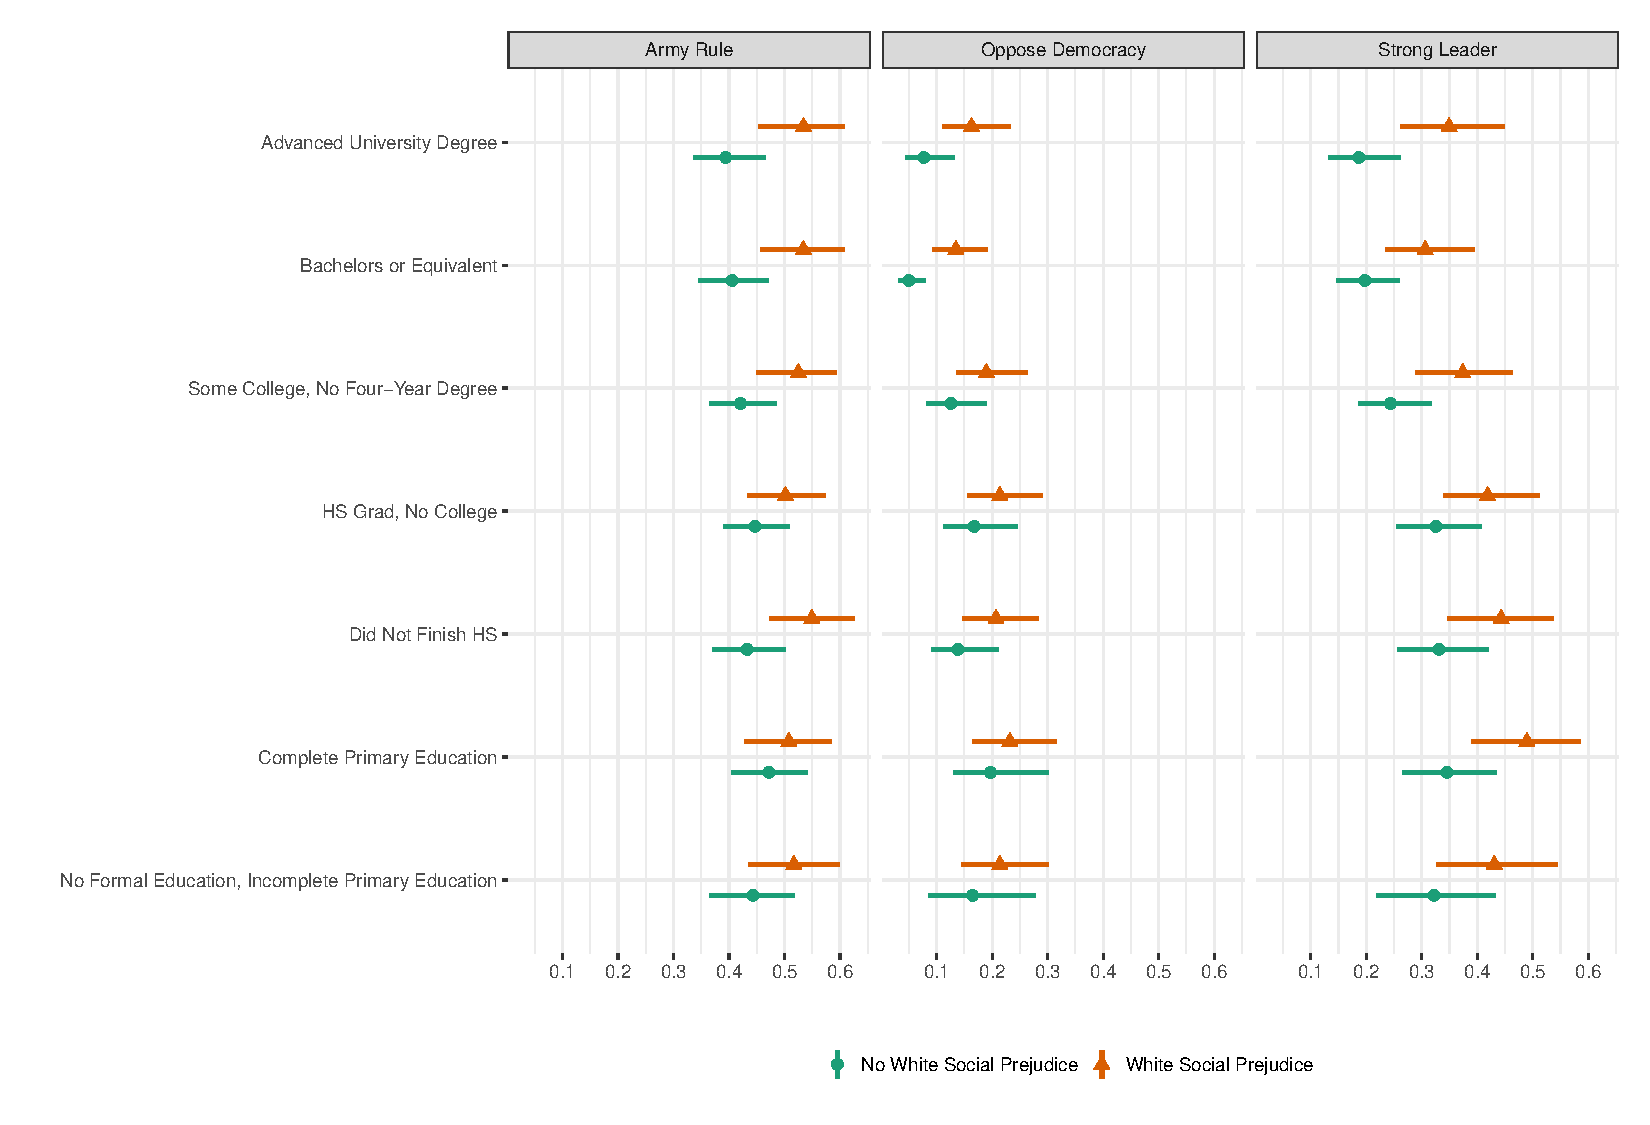
\includegraphics{figs/educ_randomslopesplot.pdf}
\caption{\label{fig:randomslopesplot}The Effect of White Social
Prejudice (as Random Slopes), by Level of Education, on Anti-Democratic
Orientations}
\end{figure}

The simulations offer further illustrative evidence that the effect of
white social prejudice may be stronger at higher levels of education.
Notice that white social prejudice appears to have little effect at
lower levels of education. Consider the categories for white Americans
who never had any exposure to college. The simulations all unequivocally
suggest a positive effect of white social prejudice; i.e.~white social
prejudice increases the likelihood of an anti-democratic orientation
even at lower levels of education. However, the effect is rather small
and the 95\% intervals surrounding the mean probability from most
simulations clearly overlap between those who are tolerant and those
whore are intolerant of immigrants/foreign workers, members of a
different race, and people who speak a different language. Only one
category in our simulations of white Americans at lower levels of
education appeared to show a near discernible difference between the
tolerant and intolerant. White social prejudice appears to noticeably
increase the likelihood of a preference for rule of government by the
U.S. army among high school dropouts. This is the lone category that
emerges from our simulations of white social prejudice's effect at lower
levels of education. Differences start to become clearer among the
college-educated. There is no overlap in the simulated effect of white
social prejudice among those with a bachelors degree or equivalent in
the model estimating opposition to democracy or support for army rule. A
similar effect is observed in the effect of white social prejudice in
supporting a strong leader for those with an advanced university degree.

Differences start to become clearer at higher levels of education among
those with at least some exposure to college. The effect of white social
prejudice starts to appear among those with at least some college
experience in the army rule and strong leader models, certainly
comparing the effect in that category relative to those with a high
school diploma and no college experience whatsoever. We start to see
clear and discernible differences among the college graduates. There is
no overlap in the simulated effect of white social prejudice among those
with a bachelors degree or equivalent in the model estimating opposition
to democracy. We see only a little overlap in the model estimating
support for army rule. We see similar discernible effects emerge among
those with an advanced university degree. The 95\% intervals do not
overlap in the strong leader model, which suggests a clear and
discernible effect of white social prejudice on attitudes in support of
strongman rule among the most educated white people in the United
States. We see only slight overlap in the model estimating support for
rule of government by the U.S. army among those with an advanced
university degree.

The simulations suggest the effect of white social prejudice may be
stronger (i.e.~more precise and more reliably positive) at higher levels
of education. Notice that the distribution of simulated first
differences is not as reliably positive at lower levels of education.
More than 15\% of the first differences from our simulations are
negative for the effect of white social prejudice on those with no
formal/incomplete primary education and those who stopped schooling
after completing the equivalent of grade school for the two models
evaluating support for rule of government by the army and outright
opposition to having a democracy in the United States. At higher levels
of education, our simulations more reliably yield results in which white
social prejudice leads to a greater likelihood of an anti-democratic
orientation. There is only one of those ridges for those with at least a
high school education in which more than five percent of the simulated
first differences were negative. That was for the simulations for those
with a high school education (and no college experience) in the army
rule estimation.

Notice the top two rows for each of the three models. These are
simulated first differences for the effect of white social prejudice on
an anti-democratic orientation for those with a four-year university
degree and those with an advanced university degree. The first
differences here are overwhelmingly positive; indeed there were none in
which more than five percent of the simulated first differences were
negative. However, it is striking how precisely positive they are. For
example, only four in 1,000 total simulations for those with advanced
university degrees yielded negative first differences in the opposition
to democracy estimation and none were negative for those with a
four-year university degree. There were only seven simulations in which
there were negative first differences in the support for strongman rule
equation, and no simulated first difference was negative for those with
an advanced university degree. Overall, the simulated first differences
are less likely to be negative as the level of education increases,
which offers more clarification and more precision of what Figure
\ref{fig:interplot} shows. It may be easy to think that social prejudice
may be a force magnifier for those with lower levels of education, but
our analysis suggests this is not quite the case. Though increasing
education does coincide with increasing support for democracy in the
U.S. (i.e.~a lower likelihood of an anti-democratic orientation in our
model), the effect of white social prejudice appears to be stronger at
higher, not lower, levels of education.

\hypertarget{robustness-tests-and-alternate-specifications}{%
\section{Robustness Tests and Alternate
Specifications}\label{robustness-tests-and-alternate-specifications}}

We use this section of the appendix to detail some robustness tests we
ran to check how sensitive our inferences are to the models we ran. We
also use this section to include full results of some abbreviated models
we ran and displayed in the manuscript. We facilitate the reader's
experience with this appendix by offering informative subsections so
that the reader can jump to a particular analysis from the table of
contents we include on the first page. We will also summarize the main
takeaways from our robustness tests in list format.

\begin{itemize}
\tightlist
\item
  Our findings are not sensitive to the choice of optimizer. We conduct
  numerous robustness tests of our main models to illlustrate this.
\item
  There is no robust effect of social prejudice on anti-democratic
  orientations for non-white respondents in the WVS data. This offers an
  empirical justification for our argument about white social prejudice
  in the United States.
\item
  We experiment with different estimations of the white social prejudice
  measure. There is no robust effect of attitudes toward Muslims or Jews
  as potential neighbors on anti-democratic orientations, though these
  categories were no longer listed after the fourth wave in 1999. The
  ``militant minority'' option is biased in the measurement sense and
  its effect on anti-democratic orientations actually drifts negative.
  Anti-LGBT responses do have positive and significant effects in two of
  three models. These four alternate options, when included in our white
  social prejudice measure, do not change the inferences we report in
  the manuscript. Importantly, re-estimating our models while looping
  through all the neighbor prompts do not consistently yield discernible
  effects on anti-democratic orientations and that a respondent saying
  s/he would not want, for example, a heavy drinker or an emotionally
  unstable person is not enough to induce opposition to democracy or
  support for authoritarian alternatives.
\item
  We experiment with seven different estimations that account for
  concerns of spatial and temporal heterogeneity in the data. These
  include a combination of fixed effects, random effects, and subsetting
  the data to just the particular survey wave. Our findings are
  remarkably robust to almost all estimations. There were only two cases
  in which we could not reject the null hypothesis: the oppose-democracy
  model in 1995 and the army-rule model in 1999. However, we think it
  important to highlight this a successful replication rate of 91.67\%
  in the combined 24 models we report in Figure
  \ref{fig:fuckitwelldoitlive}.
\end{itemize}

\hypertarget{optimizer-checks}{%
\subsection{Optimizer Checks}\label{optimizer-checks}}

We start with a brief discussion of the parameter optimization for the
models we ran and present in the manuscript. We ran a series of
generalized linear mixed effects models with weakly informative Wishart
priors on the covariance matrices. For convenience, we opted for
parameter optimization through the bound optimization by quadratic
approximation (\texttt{BOBYQA}) method \citep[c.f.][]{powell2009bobyqa}.
The standard generalized linear mixed effects model estimation does
parameter optimization through a combination of \texttt{BOBYQA} and the
\citet{neldermead1965smfm} ``downhill simplex'' method. This approach is
``standard'' for estimation but, in practice, creates much longer
computation times as the optimization goes through a series of
convergence checks.

We test whether this optimization choice we made for convenience may
have changed the results of our model. We re-estimated the three models
we report in the manuscript with a battery of different optimizers.
These are the aforementioned Nelder-Mead method and \texttt{BOBYQA}
methods. We also use the same models but permit additional stopping
criteria through non-linear optimization (\texttt{nlopt}) if the
optimization procedures believes it has found the optimum. This speeds
up computation at the expense of additional convergence checks.
Additional optimization methods include large-scale, quasi-Newton,
bound-constrained optimization of the \citet{byrdetal1995lma} method
(\texttt{L-BFGS-B}), iterative derivative-free \emph{k}-bounded
optimization of the \citet{neldermead1965smfm} method (\texttt{nmkb})
\citep{kelley1999imo}, and non-linear minimization with box constraints
(\texttt{nlminb}) \citep[c.f.][]{facchineietal1998asna}.

We briefly communicate how these different optimizers do not at all
influence the results. Figure \ref{fig:optimllk} is a comparison of the
log-likelihoods for these different optimizers across the three main
models we report in the manuscript. Figure \ref{fig:optimwnneighb}
compares the coefficient and standard errors (95\% intervals) for the
white social prejudice variable across these multiple parameter
optimizations. Notice there is almost zero difference across these
different parameter optimizations. This suggests the results we report
in the manuscript are not sensitive to the parameter optimization we
chose for computational convenience.

\begin{figure}
\centering
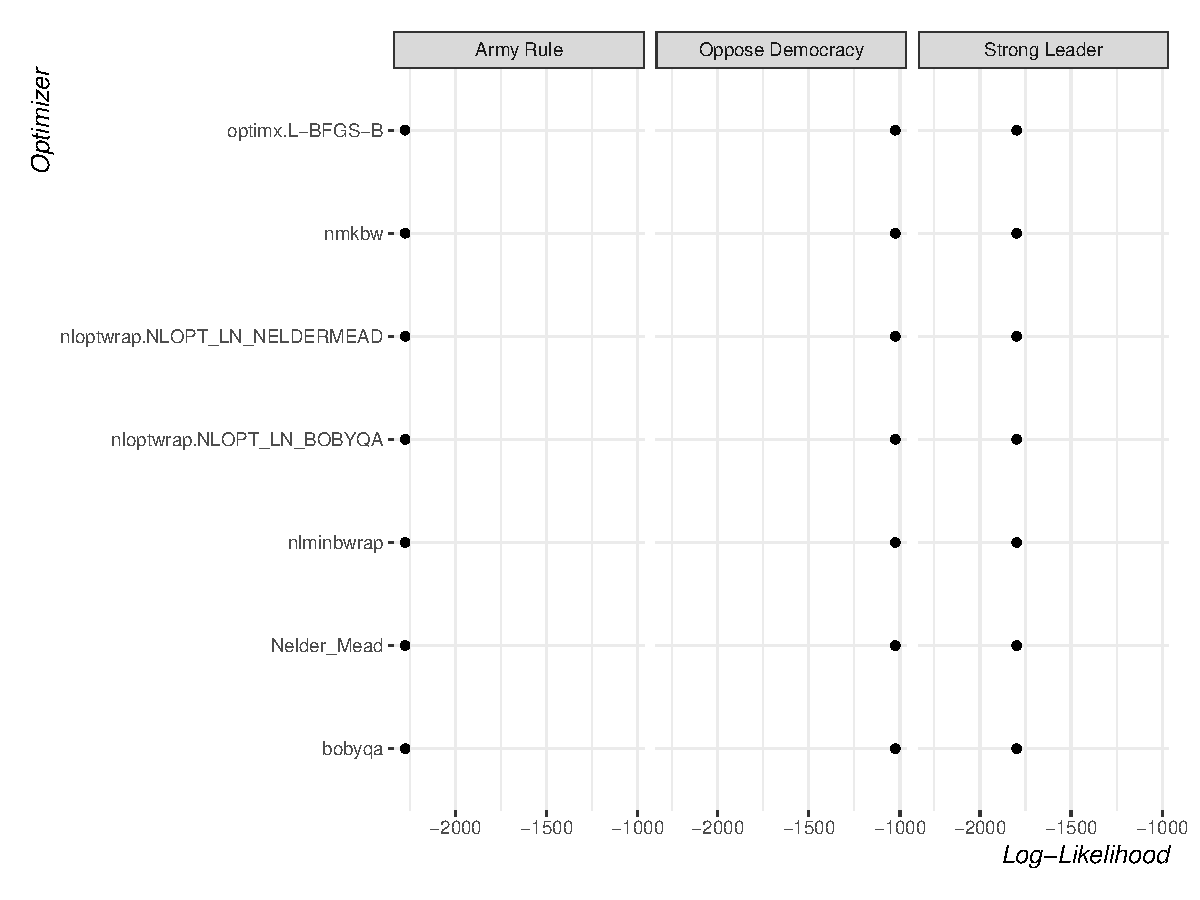
\includegraphics{figs/optimllk.pdf}
\caption{\label{fig:optimllk}A Comparison of the Log-Likelihoods from
Different Parameter Optimization Procedures}
\end{figure}

\begin{figure}
\centering
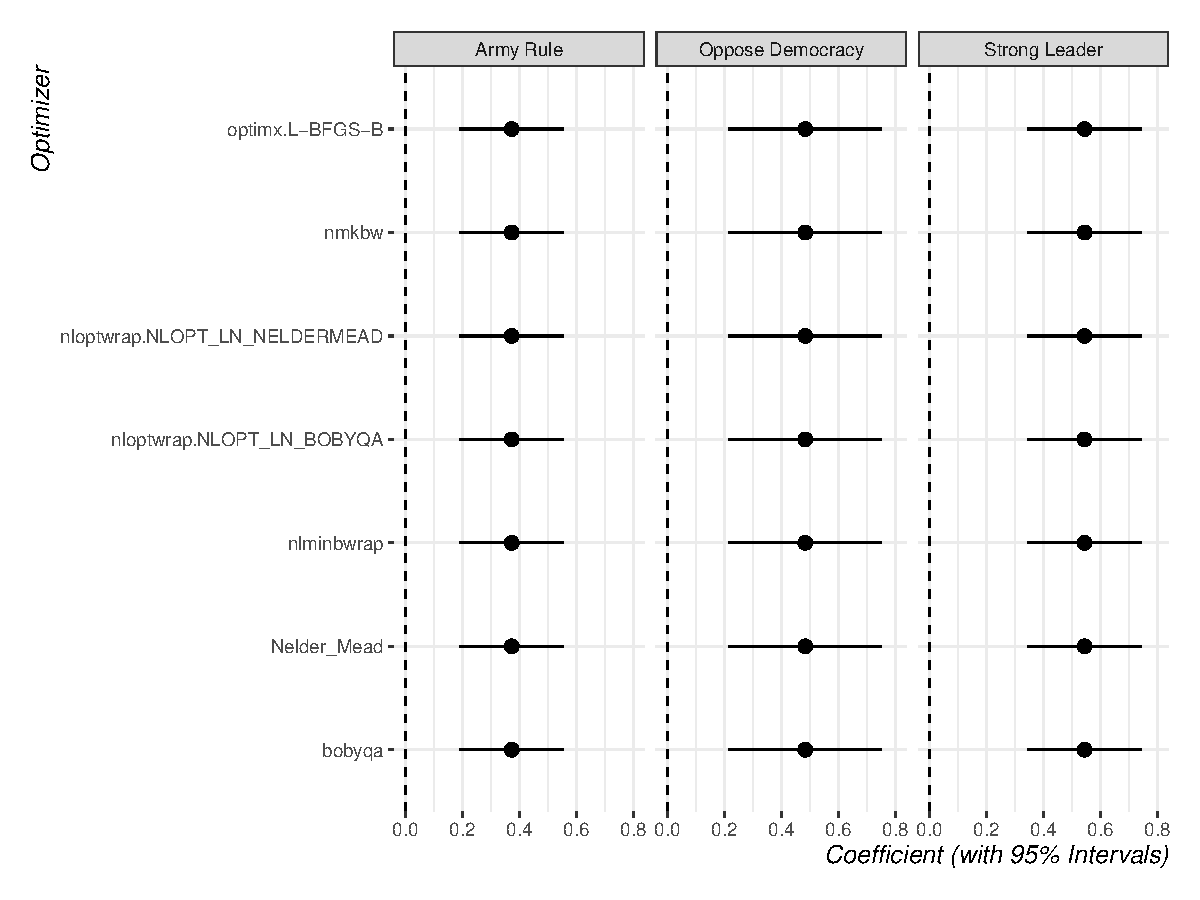
\includegraphics{figs/optimwnneighb.pdf}
\caption{\label{fig:optimwnneighb}A Comparison of the Coefficients and
Standard Errors for the White Social Prejudice Variable from Different
Parameter Optimization Procedures}
\end{figure}

\hypertarget{there-is-no-robust-effect-of-social-prejudice-on-non-white-respondents}{%
\subsection{There Is No Robust Effect of Social Prejudice on Non-White
Respondents}\label{there-is-no-robust-effect-of-social-prejudice-on-non-white-respondents}}

Our theoretical argument focuses on white Americans and we justify this
in the manuscript with our review of U.S. history and academic
literature on prejudice and tolerance. However, there is good reason to
wonder if the effect is generalizable to all Americans, even those who
are not white. This is especially important given that the reader could
interpret our argument about democracy as opportunity of access as
cutting both ways.

 
  \providecommand{\huxb}[2]{\arrayrulecolor[RGB]{#1}\global\arrayrulewidth=#2pt}
  \providecommand{\huxvb}[2]{\color[RGB]{#1}\vrule width #2pt}
  \providecommand{\huxtpad}[1]{\rule{0pt}{\baselineskip+#1}}
  \providecommand{\huxbpad}[1]{\rule[-#1]{0pt}{#1}}

\begin{table}[!htbp]
\centering
\begin{threeparttable}
\captionsetup{justification=centering,singlelinecheck=off}
\caption{\label{tab:nwmodelstab}The Covariates of Democratic Orientations of Non-White Americans in the World Values Survey (1995-2011)}
\begin{tabularx}{0.8\textwidth}{p{0.2\textwidth} p{0.2\textwidth} p{0.2\textwidth} p{0.2\textwidth}}


\hhline{>{\huxb{0, 0, 0}{0.8}}->{\huxb{0, 0, 0}{0.8}}->{\huxb{0, 0, 0}{0.8}}->{\huxb{0, 0, 0}{0.8}}-}
\arrayrulecolor{black}

\multicolumn{1}{!{\huxvb{0, 0, 0}{0}}c!{\huxvb{0, 0, 0}{0}}}{\huxtpad{4pt}\centering \huxbpad{4pt}} &
\multicolumn{1}{c!{\huxvb{0, 0, 0}{0}}}{\huxtpad{4pt}\centering \textbf{AM1}\huxbpad{4pt}} &
\multicolumn{1}{c!{\huxvb{0, 0, 0}{0}}}{\huxtpad{4pt}\centering \textbf{AM2}\huxbpad{4pt}} &
\multicolumn{1}{c!{\huxvb{0, 0, 0}{0}}}{\huxtpad{4pt}\centering \textbf{AM3}\huxbpad{4pt}} \tabularnewline[-0.5pt]


\hhline{>{\huxb{255, 255, 255}{0.4}}->{\huxb{0, 0, 0}{0.4}}->{\huxb{0, 0, 0}{0.4}}->{\huxb{0, 0, 0}{0.4}}-}
\arrayrulecolor{black}

\multicolumn{1}{!{\huxvb{0, 0, 0}{0}}c!{\huxvb{0, 0, 0}{0}}}{\huxtpad{4pt}\centering \huxbpad{4pt}} &
\multicolumn{1}{c!{\huxvb{0, 0, 0}{0}}}{\huxtpad{4pt}\centering \textit{Strong}\huxbpad{4pt}} &
\multicolumn{1}{c!{\huxvb{0, 0, 0}{0}}}{\huxtpad{4pt}\centering \textit{Army}\huxbpad{4pt}} &
\multicolumn{1}{c!{\huxvb{0, 0, 0}{0}}}{\huxtpad{4pt}\centering \textit{Oppose}\huxbpad{4pt}} \tabularnewline[-0.5pt]


\hhline{}
\arrayrulecolor{black}

\multicolumn{1}{!{\huxvb{0, 0, 0}{0}}c!{\huxvb{0, 0, 0}{0}}}{\huxtpad{4pt}\centering \huxbpad{4pt}} &
\multicolumn{1}{c!{\huxvb{0, 0, 0}{0}}}{\huxtpad{4pt}\centering \textit{Leader}\huxbpad{4pt}} &
\multicolumn{1}{c!{\huxvb{0, 0, 0}{0}}}{\huxtpad{4pt}\centering \textit{Rule}\huxbpad{4pt}} &
\multicolumn{1}{c!{\huxvb{0, 0, 0}{0}}}{\huxtpad{4pt}\centering \textit{Democracy}\huxbpad{4pt}} \tabularnewline[-0.5pt]


\hhline{>{\huxb{0, 0, 0}{0.4}}->{\huxb{0, 0, 0}{0.4}}->{\huxb{0, 0, 0}{0.4}}->{\huxb{0, 0, 0}{0.4}}-}
\arrayrulecolor{black}

\multicolumn{1}{!{\huxvb{0, 0, 0}{0}}c!{\huxvb{0, 0, 0}{0}}}{\huxtpad{4pt}\centering \huxbpad{4pt}} &
\multicolumn{1}{c!{\huxvb{0, 0, 0}{0}}}{\huxtpad{4pt}\centering \huxbpad{4pt}} &
\multicolumn{1}{c!{\huxvb{0, 0, 0}{0}}}{\huxtpad{4pt}\centering \huxbpad{4pt}} &
\multicolumn{1}{c!{\huxvb{0, 0, 0}{0}}}{\huxtpad{4pt}\centering \huxbpad{4pt}} \tabularnewline[-0.5pt]


\hhline{}
\arrayrulecolor{black}

\multicolumn{1}{!{\huxvb{0, 0, 0}{0}}l!{\huxvb{0, 0, 0}{0}}}{\huxtpad{4pt}\raggedright Age\huxbpad{4pt}} &
\multicolumn{1}{c!{\huxvb{0, 0, 0}{0}}}{\huxtpad{4pt}\centering -0.436 **\huxbpad{4pt}} &
\multicolumn{1}{c!{\huxvb{0, 0, 0}{0}}}{\huxtpad{4pt}\centering -0.323 *\huxbpad{4pt}} &
\multicolumn{1}{c!{\huxvb{0, 0, 0}{0}}}{\huxtpad{4pt}\centering -0.863 ***\huxbpad{4pt}} \tabularnewline[-0.5pt]


\hhline{}
\arrayrulecolor{black}

\multicolumn{1}{!{\huxvb{0, 0, 0}{0}}l!{\huxvb{0, 0, 0}{0}}}{\huxtpad{4pt}\raggedright \huxbpad{4pt}} &
\multicolumn{1}{c!{\huxvb{0, 0, 0}{0}}}{\huxtpad{4pt}\centering (0.145)\huxbpad{4pt}} &
\multicolumn{1}{c!{\huxvb{0, 0, 0}{0}}}{\huxtpad{4pt}\centering (0.139)\huxbpad{4pt}} &
\multicolumn{1}{c!{\huxvb{0, 0, 0}{0}}}{\huxtpad{4pt}\centering (0.261)\huxbpad{4pt}} \tabularnewline[-0.5pt]


\hhline{}
\arrayrulecolor{black}

\multicolumn{1}{!{\huxvb{0, 0, 0}{0}}l!{\huxvb{0, 0, 0}{0}}}{\huxtpad{4pt}\raggedright Age\verb|^|2\huxbpad{4pt}} &
\multicolumn{1}{c!{\huxvb{0, 0, 0}{0}}}{\huxtpad{4pt}\centering 0.061\huxbpad{4pt}} &
\multicolumn{1}{c!{\huxvb{0, 0, 0}{0}}}{\huxtpad{4pt}\centering 0.162\huxbpad{4pt}} &
\multicolumn{1}{c!{\huxvb{0, 0, 0}{0}}}{\huxtpad{4pt}\centering -0.501\huxbpad{4pt}} \tabularnewline[-0.5pt]


\hhline{}
\arrayrulecolor{black}

\multicolumn{1}{!{\huxvb{0, 0, 0}{0}}l!{\huxvb{0, 0, 0}{0}}}{\huxtpad{4pt}\raggedright \huxbpad{4pt}} &
\multicolumn{1}{c!{\huxvb{0, 0, 0}{0}}}{\huxtpad{4pt}\centering (0.277)\huxbpad{4pt}} &
\multicolumn{1}{c!{\huxvb{0, 0, 0}{0}}}{\huxtpad{4pt}\centering (0.267)\huxbpad{4pt}} &
\multicolumn{1}{c!{\huxvb{0, 0, 0}{0}}}{\huxtpad{4pt}\centering (0.475)\huxbpad{4pt}} \tabularnewline[-0.5pt]


\hhline{}
\arrayrulecolor{black}

\multicolumn{1}{!{\huxvb{0, 0, 0}{0}}l!{\huxvb{0, 0, 0}{0}}}{\huxtpad{4pt}\raggedright Female\huxbpad{4pt}} &
\multicolumn{1}{c!{\huxvb{0, 0, 0}{0}}}{\huxtpad{4pt}\centering 0.104\huxbpad{4pt}} &
\multicolumn{1}{c!{\huxvb{0, 0, 0}{0}}}{\huxtpad{4pt}\centering -0.043\huxbpad{4pt}} &
\multicolumn{1}{c!{\huxvb{0, 0, 0}{0}}}{\huxtpad{4pt}\centering 0.244\huxbpad{4pt}} \tabularnewline[-0.5pt]


\hhline{}
\arrayrulecolor{black}

\multicolumn{1}{!{\huxvb{0, 0, 0}{0}}l!{\huxvb{0, 0, 0}{0}}}{\huxtpad{4pt}\raggedright \huxbpad{4pt}} &
\multicolumn{1}{c!{\huxvb{0, 0, 0}{0}}}{\huxtpad{4pt}\centering (0.131)\huxbpad{4pt}} &
\multicolumn{1}{c!{\huxvb{0, 0, 0}{0}}}{\huxtpad{4pt}\centering (0.127)\huxbpad{4pt}} &
\multicolumn{1}{c!{\huxvb{0, 0, 0}{0}}}{\huxtpad{4pt}\centering (0.195)\huxbpad{4pt}} \tabularnewline[-0.5pt]


\hhline{}
\arrayrulecolor{black}

\multicolumn{1}{!{\huxvb{0, 0, 0}{0}}l!{\huxvb{0, 0, 0}{0}}}{\huxtpad{4pt}\raggedright College Educated\huxbpad{4pt}} &
\multicolumn{1}{c!{\huxvb{0, 0, 0}{0}}}{\huxtpad{4pt}\centering -0.434 *\huxbpad{4pt}} &
\multicolumn{1}{c!{\huxvb{0, 0, 0}{0}}}{\huxtpad{4pt}\centering -0.061\huxbpad{4pt}} &
\multicolumn{1}{c!{\huxvb{0, 0, 0}{0}}}{\huxtpad{4pt}\centering -1.475 ***\huxbpad{4pt}} \tabularnewline[-0.5pt]


\hhline{}
\arrayrulecolor{black}

\multicolumn{1}{!{\huxvb{0, 0, 0}{0}}l!{\huxvb{0, 0, 0}{0}}}{\huxtpad{4pt}\raggedright \huxbpad{4pt}} &
\multicolumn{1}{c!{\huxvb{0, 0, 0}{0}}}{\huxtpad{4pt}\centering (0.172)\huxbpad{4pt}} &
\multicolumn{1}{c!{\huxvb{0, 0, 0}{0}}}{\huxtpad{4pt}\centering (0.163)\huxbpad{4pt}} &
\multicolumn{1}{c!{\huxvb{0, 0, 0}{0}}}{\huxtpad{4pt}\centering (0.370)\huxbpad{4pt}} \tabularnewline[-0.5pt]


\hhline{}
\arrayrulecolor{black}

\multicolumn{1}{!{\huxvb{0, 0, 0}{0}}l!{\huxvb{0, 0, 0}{0}}}{\huxtpad{4pt}\raggedright Ideology\huxbpad{4pt}} &
\multicolumn{1}{c!{\huxvb{0, 0, 0}{0}}}{\huxtpad{4pt}\centering 0.219\huxbpad{4pt}} &
\multicolumn{1}{c!{\huxvb{0, 0, 0}{0}}}{\huxtpad{4pt}\centering 0.007\huxbpad{4pt}} &
\multicolumn{1}{c!{\huxvb{0, 0, 0}{0}}}{\huxtpad{4pt}\centering -0.014\huxbpad{4pt}} \tabularnewline[-0.5pt]


\hhline{}
\arrayrulecolor{black}

\multicolumn{1}{!{\huxvb{0, 0, 0}{0}}l!{\huxvb{0, 0, 0}{0}}}{\huxtpad{4pt}\raggedright \huxbpad{4pt}} &
\multicolumn{1}{c!{\huxvb{0, 0, 0}{0}}}{\huxtpad{4pt}\centering (0.134)\huxbpad{4pt}} &
\multicolumn{1}{c!{\huxvb{0, 0, 0}{0}}}{\huxtpad{4pt}\centering (0.129)\huxbpad{4pt}} &
\multicolumn{1}{c!{\huxvb{0, 0, 0}{0}}}{\huxtpad{4pt}\centering (0.192)\huxbpad{4pt}} \tabularnewline[-0.5pt]


\hhline{}
\arrayrulecolor{black}

\multicolumn{1}{!{\huxvb{0, 0, 0}{0}}l!{\huxvb{0, 0, 0}{0}}}{\huxtpad{4pt}\raggedright Ideology\verb|^|2\huxbpad{4pt}} &
\multicolumn{1}{c!{\huxvb{0, 0, 0}{0}}}{\huxtpad{4pt}\centering -0.175\huxbpad{4pt}} &
\multicolumn{1}{c!{\huxvb{0, 0, 0}{0}}}{\huxtpad{4pt}\centering -0.142\huxbpad{4pt}} &
\multicolumn{1}{c!{\huxvb{0, 0, 0}{0}}}{\huxtpad{4pt}\centering 0.300\huxbpad{4pt}} \tabularnewline[-0.5pt]


\hhline{}
\arrayrulecolor{black}

\multicolumn{1}{!{\huxvb{0, 0, 0}{0}}l!{\huxvb{0, 0, 0}{0}}}{\huxtpad{4pt}\raggedright \huxbpad{4pt}} &
\multicolumn{1}{c!{\huxvb{0, 0, 0}{0}}}{\huxtpad{4pt}\centering (0.168)\huxbpad{4pt}} &
\multicolumn{1}{c!{\huxvb{0, 0, 0}{0}}}{\huxtpad{4pt}\centering (0.160)\huxbpad{4pt}} &
\multicolumn{1}{c!{\huxvb{0, 0, 0}{0}}}{\huxtpad{4pt}\centering (0.232)\huxbpad{4pt}} \tabularnewline[-0.5pt]


\hhline{}
\arrayrulecolor{black}

\multicolumn{1}{!{\huxvb{0, 0, 0}{0}}l!{\huxvb{0, 0, 0}{0}}}{\huxtpad{4pt}\raggedright Income Scale\huxbpad{4pt}} &
\multicolumn{1}{c!{\huxvb{0, 0, 0}{0}}}{\huxtpad{4pt}\centering 0.034\huxbpad{4pt}} &
\multicolumn{1}{c!{\huxvb{0, 0, 0}{0}}}{\huxtpad{4pt}\centering -0.248\huxbpad{4pt}} &
\multicolumn{1}{c!{\huxvb{0, 0, 0}{0}}}{\huxtpad{4pt}\centering 0.154\huxbpad{4pt}} \tabularnewline[-0.5pt]


\hhline{}
\arrayrulecolor{black}

\multicolumn{1}{!{\huxvb{0, 0, 0}{0}}l!{\huxvb{0, 0, 0}{0}}}{\huxtpad{4pt}\raggedright \huxbpad{4pt}} &
\multicolumn{1}{c!{\huxvb{0, 0, 0}{0}}}{\huxtpad{4pt}\centering (0.143)\huxbpad{4pt}} &
\multicolumn{1}{c!{\huxvb{0, 0, 0}{0}}}{\huxtpad{4pt}\centering (0.139)\huxbpad{4pt}} &
\multicolumn{1}{c!{\huxvb{0, 0, 0}{0}}}{\huxtpad{4pt}\centering (0.210)\huxbpad{4pt}} \tabularnewline[-0.5pt]


\hhline{}
\arrayrulecolor{black}

\multicolumn{1}{!{\huxvb{0, 0, 0}{0}}l!{\huxvb{0, 0, 0}{0}}}{\huxtpad{4pt}\raggedright Republican\huxbpad{4pt}} &
\multicolumn{1}{c!{\huxvb{0, 0, 0}{0}}}{\huxtpad{4pt}\centering -0.143\huxbpad{4pt}} &
\multicolumn{1}{c!{\huxvb{0, 0, 0}{0}}}{\huxtpad{4pt}\centering 0.053\huxbpad{4pt}} &
\multicolumn{1}{c!{\huxvb{0, 0, 0}{0}}}{\huxtpad{4pt}\centering -0.347\huxbpad{4pt}} \tabularnewline[-0.5pt]


\hhline{}
\arrayrulecolor{black}

\multicolumn{1}{!{\huxvb{0, 0, 0}{0}}l!{\huxvb{0, 0, 0}{0}}}{\huxtpad{4pt}\raggedright \huxbpad{4pt}} &
\multicolumn{1}{c!{\huxvb{0, 0, 0}{0}}}{\huxtpad{4pt}\centering (0.264)\huxbpad{4pt}} &
\multicolumn{1}{c!{\huxvb{0, 0, 0}{0}}}{\huxtpad{4pt}\centering (0.254)\huxbpad{4pt}} &
\multicolumn{1}{c!{\huxvb{0, 0, 0}{0}}}{\huxtpad{4pt}\centering (0.319)\huxbpad{4pt}} \tabularnewline[-0.5pt]


\hhline{}
\arrayrulecolor{black}

\multicolumn{1}{!{\huxvb{0, 0, 0}{0}}l!{\huxvb{0, 0, 0}{0}}}{\huxtpad{4pt}\raggedright Democrat\huxbpad{4pt}} &
\multicolumn{1}{c!{\huxvb{0, 0, 0}{0}}}{\huxtpad{4pt}\centering 0.314\huxbpad{4pt}} &
\multicolumn{1}{c!{\huxvb{0, 0, 0}{0}}}{\huxtpad{4pt}\centering 0.014\huxbpad{4pt}} &
\multicolumn{1}{c!{\huxvb{0, 0, 0}{0}}}{\huxtpad{4pt}\centering -1.107 ***\huxbpad{4pt}} \tabularnewline[-0.5pt]


\hhline{}
\arrayrulecolor{black}

\multicolumn{1}{!{\huxvb{0, 0, 0}{0}}l!{\huxvb{0, 0, 0}{0}}}{\huxtpad{4pt}\raggedright \huxbpad{4pt}} &
\multicolumn{1}{c!{\huxvb{0, 0, 0}{0}}}{\huxtpad{4pt}\centering (0.221)\huxbpad{4pt}} &
\multicolumn{1}{c!{\huxvb{0, 0, 0}{0}}}{\huxtpad{4pt}\centering (0.213)\huxbpad{4pt}} &
\multicolumn{1}{c!{\huxvb{0, 0, 0}{0}}}{\huxtpad{4pt}\centering (0.269)\huxbpad{4pt}} \tabularnewline[-0.5pt]


\hhline{}
\arrayrulecolor{black}

\multicolumn{1}{!{\huxvb{0, 0, 0}{0}}l!{\huxvb{0, 0, 0}{0}}}{\huxtpad{4pt}\raggedright Unemployed\huxbpad{4pt}} &
\multicolumn{1}{c!{\huxvb{0, 0, 0}{0}}}{\huxtpad{4pt}\centering 0.635 **\huxbpad{4pt}} &
\multicolumn{1}{c!{\huxvb{0, 0, 0}{0}}}{\huxtpad{4pt}\centering 0.134\huxbpad{4pt}} &
\multicolumn{1}{c!{\huxvb{0, 0, 0}{0}}}{\huxtpad{4pt}\centering 0.447\huxbpad{4pt}} \tabularnewline[-0.5pt]


\hhline{}
\arrayrulecolor{black}

\multicolumn{1}{!{\huxvb{0, 0, 0}{0}}l!{\huxvb{0, 0, 0}{0}}}{\huxtpad{4pt}\raggedright \huxbpad{4pt}} &
\multicolumn{1}{c!{\huxvb{0, 0, 0}{0}}}{\huxtpad{4pt}\centering (0.231)\huxbpad{4pt}} &
\multicolumn{1}{c!{\huxvb{0, 0, 0}{0}}}{\huxtpad{4pt}\centering (0.220)\huxbpad{4pt}} &
\multicolumn{1}{c!{\huxvb{0, 0, 0}{0}}}{\huxtpad{4pt}\centering (0.281)\huxbpad{4pt}} \tabularnewline[-0.5pt]


\hhline{}
\arrayrulecolor{black}

\multicolumn{1}{!{\huxvb{0, 0, 0}{0}}l!{\huxvb{0, 0, 0}{0}}}{\huxtpad{4pt}\raggedright Emancipative Values\huxbpad{4pt}} &
\multicolumn{1}{c!{\huxvb{0, 0, 0}{0}}}{\huxtpad{4pt}\centering -0.494 ***\huxbpad{4pt}} &
\multicolumn{1}{c!{\huxvb{0, 0, 0}{0}}}{\huxtpad{4pt}\centering -0.120\huxbpad{4pt}} &
\multicolumn{1}{c!{\huxvb{0, 0, 0}{0}}}{\huxtpad{4pt}\centering -0.398\huxbpad{4pt}} \tabularnewline[-0.5pt]


\hhline{}
\arrayrulecolor{black}

\multicolumn{1}{!{\huxvb{0, 0, 0}{0}}l!{\huxvb{0, 0, 0}{0}}}{\huxtpad{4pt}\raggedright \huxbpad{4pt}} &
\multicolumn{1}{c!{\huxvb{0, 0, 0}{0}}}{\huxtpad{4pt}\centering (0.148)\huxbpad{4pt}} &
\multicolumn{1}{c!{\huxvb{0, 0, 0}{0}}}{\huxtpad{4pt}\centering (0.141)\huxbpad{4pt}} &
\multicolumn{1}{c!{\huxvb{0, 0, 0}{0}}}{\huxtpad{4pt}\centering (0.214)\huxbpad{4pt}} \tabularnewline[-0.5pt]


\hhline{}
\arrayrulecolor{black}

\multicolumn{1}{!{\huxvb{0, 0, 0}{0}}l!{\huxvb{0, 0, 0}{0}}}{\huxtpad{4pt}\raggedright Social Prejudice\huxbpad{4pt}} &
\multicolumn{1}{c!{\huxvb{0, 0, 0}{0}}}{\huxtpad{4pt}\centering 0.625 **\huxbpad{4pt}} &
\multicolumn{1}{c!{\huxvb{0, 0, 0}{0}}}{\huxtpad{4pt}\centering 0.293\huxbpad{4pt}} &
\multicolumn{1}{c!{\huxvb{0, 0, 0}{0}}}{\huxtpad{4pt}\centering 0.307\huxbpad{4pt}} \tabularnewline[-0.5pt]


\hhline{}
\arrayrulecolor{black}

\multicolumn{1}{!{\huxvb{0, 0, 0}{0}}l!{\huxvb{0, 0, 0}{0}}}{\huxtpad{4pt}\raggedright \huxbpad{4pt}} &
\multicolumn{1}{c!{\huxvb{0, 0, 0}{0}}}{\huxtpad{4pt}\centering (0.201)\huxbpad{4pt}} &
\multicolumn{1}{c!{\huxvb{0, 0, 0}{0}}}{\huxtpad{4pt}\centering (0.198)\huxbpad{4pt}} &
\multicolumn{1}{c!{\huxvb{0, 0, 0}{0}}}{\huxtpad{4pt}\centering (0.273)\huxbpad{4pt}} \tabularnewline[-0.5pt]


\hhline{}
\arrayrulecolor{black}

\multicolumn{1}{!{\huxvb{0, 0, 0}{0}}l!{\huxvb{0, 0, 0}{0}}}{\huxtpad{4pt}\raggedright \huxbpad{4pt}} &
\multicolumn{1}{c!{\huxvb{0, 0, 0}{0}}}{\huxtpad{4pt}\centering \huxbpad{4pt}} &
\multicolumn{1}{c!{\huxvb{0, 0, 0}{0}}}{\huxtpad{4pt}\centering \huxbpad{4pt}} &
\multicolumn{1}{c!{\huxvb{0, 0, 0}{0}}}{\huxtpad{4pt}\centering \huxbpad{4pt}} \tabularnewline[-0.5pt]


\hhline{}
\arrayrulecolor{black}

\multicolumn{1}{!{\huxvb{0, 0, 0}{0}}l!{\huxvb{0, 0, 0}{0}}}{\huxtpad{4pt}\raggedright \textit{Random Effect}\huxbpad{4pt}} &
\multicolumn{1}{c!{\huxvb{0, 0, 0}{0}}}{\huxtpad{4pt}\centering \huxbpad{4pt}} &
\multicolumn{1}{c!{\huxvb{0, 0, 0}{0}}}{\huxtpad{4pt}\centering \huxbpad{4pt}} &
\multicolumn{1}{c!{\huxvb{0, 0, 0}{0}}}{\huxtpad{4pt}\centering \huxbpad{4pt}} \tabularnewline[-0.5pt]


\hhline{}
\arrayrulecolor{black}

\multicolumn{1}{!{\huxvb{0, 0, 0}{0}}l!{\huxvb{0, 0, 0}{0}}}{\huxtpad{4pt}\raggedright sd(Year)\huxbpad{4pt}} &
\multicolumn{1}{c!{\huxvb{0, 0, 0}{0}}}{\huxtpad{4pt}\centering 0.366\huxbpad{4pt}} &
\multicolumn{1}{c!{\huxvb{0, 0, 0}{0}}}{\huxtpad{4pt}\centering 0.263\huxbpad{4pt}} &
\multicolumn{1}{c!{\huxvb{0, 0, 0}{0}}}{\huxtpad{4pt}\centering 0.222\huxbpad{4pt}} \tabularnewline[-0.5pt]


\hhline{}
\arrayrulecolor{black}

\multicolumn{1}{!{\huxvb{0, 0, 0}{0}}l!{\huxvb{0, 0, 0}{0}}}{\huxtpad{4pt}\raggedright \huxbpad{4pt}} &
\multicolumn{1}{c!{\huxvb{0, 0, 0}{0}}}{\huxtpad{4pt}\centering \huxbpad{4pt}} &
\multicolumn{1}{c!{\huxvb{0, 0, 0}{0}}}{\huxtpad{4pt}\centering \huxbpad{4pt}} &
\multicolumn{1}{c!{\huxvb{0, 0, 0}{0}}}{\huxtpad{4pt}\centering \huxbpad{4pt}} \tabularnewline[-0.5pt]


\hhline{}
\arrayrulecolor{black}

\multicolumn{1}{!{\huxvb{0, 0, 0}{0}}l!{\huxvb{0, 0, 0}{0}}}{\huxtpad{4pt}\raggedright N\huxbpad{4pt}} &
\multicolumn{1}{c!{\huxvb{0, 0, 0}{0}}}{\huxtpad{4pt}\centering 1096\huxbpad{4pt}} &
\multicolumn{1}{c!{\huxvb{0, 0, 0}{0}}}{\huxtpad{4pt}\centering 1090\huxbpad{4pt}} &
\multicolumn{1}{c!{\huxvb{0, 0, 0}{0}}}{\huxtpad{4pt}\centering 1093\huxbpad{4pt}} \tabularnewline[-0.5pt]


\hhline{>{\huxb{0, 0, 0}{0.8}}->{\huxb{0, 0, 0}{0.8}}->{\huxb{0, 0, 0}{0.8}}->{\huxb{0, 0, 0}{0.8}}-}
\arrayrulecolor{black}

\multicolumn{4}{!{\huxvb{0, 0, 0}{0}}p{0.8\textwidth+6\tabcolsep}!{\huxvb{0, 0, 0}{0}}}{\parbox[b]{0.8\textwidth+6\tabcolsep-4pt-4pt}{\huxtpad{4pt}\raggedright  *** p $<$ 0.001;  ** p $<$ 0.01;  * p $<$ 0.05.\huxbpad{4pt}}} \tabularnewline[-0.5pt]


\hhline{}
\arrayrulecolor{black}
\end{tabularx}\end{threeparttable}


\end{table}
 

We subset the data to non-white respondents across the third through
sixth waves of World Values Survey (WVS) data and re-estimated the three
main analyses we report in Figure 2 in the manuscript. The results show
there is no robust effect of social prejudice on anti-democratic
orientations for non-white respondents. Only the strong leader model
(\texttt{AM1}) had a statistically significant effect. The lower bounds
of the 95\% intervals surrounding the coefficient estimates in the army
rule and opposition to democracy models clearly overlap with zero. All
told, Table \ref{tab:nwmodelstab} offers an empirical justification of
our decision to focus on the effect of social prejudice on white
Americans. Our argument is aggrieved white Americans perceive democracy
as empowering unwelcome ethnic/racial minorities with an equal
opportunity of access to power beyond the minority's numerical
endowment. This leads to an anti-democratic orientation we observe among
white Americans if these respondents do not view these groups as welcome
in their life. However, we do not observe a robust effect of this social
prejudice for non-white Americans.

\hypertarget{alternate-estimations-of-white-social-prejudice-do-not-change-our-inferences}{%
\subsection{Alternate Estimations of White Social Prejudice Do Not
Change Our
Inferences}\label{alternate-estimations-of-white-social-prejudice-do-not-change-our-inferences}}

We also consider whether the inferences we report in the manuscript are
sensitive to the measure of white social prejudice we devised. The
ridgeline plots in the manuscript's Figure 3 show a discernible
robustness in our simulations of the 12 different models we ran. Only
one of the thousand simulations of those 12 models resulted in a
distribution of first differences in which more than 5\% of the first
differences were negative. That was the simulated first differences for
the effect of not wanting a neighbor who spoke a different language on
attitutes in opposition to democracy. Even then, just 7.6\% of those
simulated first differences were negative.

We explore the effect that some other relevant responses may have on the
anti-democratic orientations we analyze. For one, our identification of
white social prejudice leveraged responses that identified
immigrants/foreign workers, members of a different race, and people who
speak a different language as indicators of white social prejudice if
the respondent would not welcome these groups as neighbors. There are
two other responses of interest: Jews and Muslims. White nationalists
routinely single out Muslims as a threat to their perception of American
values and anti-Semitism is a long-running strand of bigotry in groups
like the Ku Klux Klan. However, our specification opted for common nouns
in lieu of proper nouns for the analyses we report in the manuscript.
Further, WVS listed Muslims as potential responses in 1995 and 1999 and
Jews as an option in the 1999 wave. They regrettably do not appear in
the post-9/11 waves in 2006 and 2011.

 
  \providecommand{\huxb}[2]{\arrayrulecolor[RGB]{#1}\global\arrayrulewidth=#2pt}
  \providecommand{\huxvb}[2]{\color[RGB]{#1}\vrule width #2pt}
  \providecommand{\huxtpad}[1]{\rule{0pt}{\baselineskip+#1}}
  \providecommand{\huxbpad}[1]{\rule[-#1]{0pt}{#1}}

\begin{table}[!htbp]
\centering
\begin{threeparttable}
\captionsetup{justification=centering,singlelinecheck=off}
\caption{\label{tab:jwmodelstab}The Covariates of Democratic Orientations of White Americans in the World Values Survey [with anti-Jews/Muslims Responses] (1995-2011)}
\begin{tabularx}{0.6\textwidth}{p{0.15\textwidth} p{0.15\textwidth} p{0.15\textwidth} p{0.15\textwidth}}


\hhline{>{\huxb{0, 0, 0}{0.8}}->{\huxb{0, 0, 0}{0.8}}->{\huxb{0, 0, 0}{0.8}}->{\huxb{0, 0, 0}{0.8}}-}
\arrayrulecolor{black}

\multicolumn{1}{!{\huxvb{0, 0, 0}{0}}c!{\huxvb{0, 0, 0}{0}}}{\huxtpad{4pt}\centering \huxbpad{4pt}} &
\multicolumn{1}{c!{\huxvb{0, 0, 0}{0}}}{\huxtpad{4pt}\centering \textbf{AM4}\huxbpad{4pt}} &
\multicolumn{1}{c!{\huxvb{0, 0, 0}{0}}}{\huxtpad{4pt}\centering \textbf{AM5}\huxbpad{4pt}} &
\multicolumn{1}{c!{\huxvb{0, 0, 0}{0}}}{\huxtpad{4pt}\centering \textbf{AM6}\huxbpad{4pt}} \tabularnewline[-0.5pt]


\hhline{>{\huxb{255, 255, 255}{0.4}}->{\huxb{0, 0, 0}{0.4}}->{\huxb{0, 0, 0}{0.4}}->{\huxb{0, 0, 0}{0.4}}-}
\arrayrulecolor{black}

\multicolumn{1}{!{\huxvb{0, 0, 0}{0}}c!{\huxvb{0, 0, 0}{0}}}{\huxtpad{4pt}\centering \huxbpad{4pt}} &
\multicolumn{1}{c!{\huxvb{0, 0, 0}{0}}}{\huxtpad{4pt}\centering \textit{Strong}\huxbpad{4pt}} &
\multicolumn{1}{c!{\huxvb{0, 0, 0}{0}}}{\huxtpad{4pt}\centering \textit{Army}\huxbpad{4pt}} &
\multicolumn{1}{c!{\huxvb{0, 0, 0}{0}}}{\huxtpad{4pt}\centering \textit{Oppose}\huxbpad{4pt}} \tabularnewline[-0.5pt]


\hhline{}
\arrayrulecolor{black}

\multicolumn{1}{!{\huxvb{0, 0, 0}{0}}c!{\huxvb{0, 0, 0}{0}}}{\huxtpad{4pt}\centering \huxbpad{4pt}} &
\multicolumn{1}{c!{\huxvb{0, 0, 0}{0}}}{\huxtpad{4pt}\centering \textit{Leader}\huxbpad{4pt}} &
\multicolumn{1}{c!{\huxvb{0, 0, 0}{0}}}{\huxtpad{4pt}\centering \textit{Rule}\huxbpad{4pt}} &
\multicolumn{1}{c!{\huxvb{0, 0, 0}{0}}}{\huxtpad{4pt}\centering \textit{Democracy}\huxbpad{4pt}} \tabularnewline[-0.5pt]


\hhline{>{\huxb{0, 0, 0}{0.4}}->{\huxb{0, 0, 0}{0.4}}->{\huxb{0, 0, 0}{0.4}}->{\huxb{0, 0, 0}{0.4}}-}
\arrayrulecolor{black}

\multicolumn{1}{!{\huxvb{0, 0, 0}{0}}c!{\huxvb{0, 0, 0}{0}}}{\huxtpad{4pt}\centering \huxbpad{4pt}} &
\multicolumn{1}{c!{\huxvb{0, 0, 0}{0}}}{\huxtpad{4pt}\centering \huxbpad{4pt}} &
\multicolumn{1}{c!{\huxvb{0, 0, 0}{0}}}{\huxtpad{4pt}\centering \huxbpad{4pt}} &
\multicolumn{1}{c!{\huxvb{0, 0, 0}{0}}}{\huxtpad{4pt}\centering \huxbpad{4pt}} \tabularnewline[-0.5pt]


\hhline{}
\arrayrulecolor{black}

\multicolumn{1}{!{\huxvb{0, 0, 0}{0}}l!{\huxvb{0, 0, 0}{0}}}{\huxtpad{4pt}\raggedright Age\huxbpad{4pt}} &
\multicolumn{1}{c!{\huxvb{0, 0, 0}{0}}}{\huxtpad{4pt}\centering -0.443 ***\huxbpad{4pt}} &
\multicolumn{1}{c!{\huxvb{0, 0, 0}{0}}}{\huxtpad{4pt}\centering -0.449 ***\huxbpad{4pt}} &
\multicolumn{1}{c!{\huxvb{0, 0, 0}{0}}}{\huxtpad{4pt}\centering -0.636 ***\huxbpad{4pt}} \tabularnewline[-0.5pt]


\hhline{}
\arrayrulecolor{black}

\multicolumn{1}{!{\huxvb{0, 0, 0}{0}}l!{\huxvb{0, 0, 0}{0}}}{\huxtpad{4pt}\raggedright \huxbpad{4pt}} &
\multicolumn{1}{c!{\huxvb{0, 0, 0}{0}}}{\huxtpad{4pt}\centering (0.087)\huxbpad{4pt}} &
\multicolumn{1}{c!{\huxvb{0, 0, 0}{0}}}{\huxtpad{4pt}\centering (0.077)\huxbpad{4pt}} &
\multicolumn{1}{c!{\huxvb{0, 0, 0}{0}}}{\huxtpad{4pt}\centering (0.120)\huxbpad{4pt}} \tabularnewline[-0.5pt]


\hhline{}
\arrayrulecolor{black}

\multicolumn{1}{!{\huxvb{0, 0, 0}{0}}l!{\huxvb{0, 0, 0}{0}}}{\huxtpad{4pt}\raggedright Age\verb|^|2\huxbpad{4pt}} &
\multicolumn{1}{c!{\huxvb{0, 0, 0}{0}}}{\huxtpad{4pt}\centering 0.155\huxbpad{4pt}} &
\multicolumn{1}{c!{\huxvb{0, 0, 0}{0}}}{\huxtpad{4pt}\centering 0.041\huxbpad{4pt}} &
\multicolumn{1}{c!{\huxvb{0, 0, 0}{0}}}{\huxtpad{4pt}\centering 0.070\huxbpad{4pt}} \tabularnewline[-0.5pt]


\hhline{}
\arrayrulecolor{black}

\multicolumn{1}{!{\huxvb{0, 0, 0}{0}}l!{\huxvb{0, 0, 0}{0}}}{\huxtpad{4pt}\raggedright \huxbpad{4pt}} &
\multicolumn{1}{c!{\huxvb{0, 0, 0}{0}}}{\huxtpad{4pt}\centering (0.158)\huxbpad{4pt}} &
\multicolumn{1}{c!{\huxvb{0, 0, 0}{0}}}{\huxtpad{4pt}\centering (0.139)\huxbpad{4pt}} &
\multicolumn{1}{c!{\huxvb{0, 0, 0}{0}}}{\huxtpad{4pt}\centering (0.223)\huxbpad{4pt}} \tabularnewline[-0.5pt]


\hhline{}
\arrayrulecolor{black}

\multicolumn{1}{!{\huxvb{0, 0, 0}{0}}l!{\huxvb{0, 0, 0}{0}}}{\huxtpad{4pt}\raggedright Female\huxbpad{4pt}} &
\multicolumn{1}{c!{\huxvb{0, 0, 0}{0}}}{\huxtpad{4pt}\centering 0.048\huxbpad{4pt}} &
\multicolumn{1}{c!{\huxvb{0, 0, 0}{0}}}{\huxtpad{4pt}\centering 0.137\huxbpad{4pt}} &
\multicolumn{1}{c!{\huxvb{0, 0, 0}{0}}}{\huxtpad{4pt}\centering 0.518 ***\huxbpad{4pt}} \tabularnewline[-0.5pt]


\hhline{}
\arrayrulecolor{black}

\multicolumn{1}{!{\huxvb{0, 0, 0}{0}}l!{\huxvb{0, 0, 0}{0}}}{\huxtpad{4pt}\raggedright \huxbpad{4pt}} &
\multicolumn{1}{c!{\huxvb{0, 0, 0}{0}}}{\huxtpad{4pt}\centering (0.084)\huxbpad{4pt}} &
\multicolumn{1}{c!{\huxvb{0, 0, 0}{0}}}{\huxtpad{4pt}\centering (0.072)\huxbpad{4pt}} &
\multicolumn{1}{c!{\huxvb{0, 0, 0}{0}}}{\huxtpad{4pt}\centering (0.118)\huxbpad{4pt}} \tabularnewline[-0.5pt]


\hhline{}
\arrayrulecolor{black}

\multicolumn{1}{!{\huxvb{0, 0, 0}{0}}l!{\huxvb{0, 0, 0}{0}}}{\huxtpad{4pt}\raggedright College Educated\huxbpad{4pt}} &
\multicolumn{1}{c!{\huxvb{0, 0, 0}{0}}}{\huxtpad{4pt}\centering -0.563 ***\huxbpad{4pt}} &
\multicolumn{1}{c!{\huxvb{0, 0, 0}{0}}}{\huxtpad{4pt}\centering -0.157\huxbpad{4pt}} &
\multicolumn{1}{c!{\huxvb{0, 0, 0}{0}}}{\huxtpad{4pt}\centering -1.033 ***\huxbpad{4pt}} \tabularnewline[-0.5pt]


\hhline{}
\arrayrulecolor{black}

\multicolumn{1}{!{\huxvb{0, 0, 0}{0}}l!{\huxvb{0, 0, 0}{0}}}{\huxtpad{4pt}\raggedright \huxbpad{4pt}} &
\multicolumn{1}{c!{\huxvb{0, 0, 0}{0}}}{\huxtpad{4pt}\centering (0.103)\huxbpad{4pt}} &
\multicolumn{1}{c!{\huxvb{0, 0, 0}{0}}}{\huxtpad{4pt}\centering (0.083)\huxbpad{4pt}} &
\multicolumn{1}{c!{\huxvb{0, 0, 0}{0}}}{\huxtpad{4pt}\centering (0.171)\huxbpad{4pt}} \tabularnewline[-0.5pt]


\hhline{}
\arrayrulecolor{black}

\multicolumn{1}{!{\huxvb{0, 0, 0}{0}}l!{\huxvb{0, 0, 0}{0}}}{\huxtpad{4pt}\raggedright Ideology\huxbpad{4pt}} &
\multicolumn{1}{c!{\huxvb{0, 0, 0}{0}}}{\huxtpad{4pt}\centering -0.007\huxbpad{4pt}} &
\multicolumn{1}{c!{\huxvb{0, 0, 0}{0}}}{\huxtpad{4pt}\centering -0.169 *\huxbpad{4pt}} &
\multicolumn{1}{c!{\huxvb{0, 0, 0}{0}}}{\huxtpad{4pt}\centering -0.265\huxbpad{4pt}} \tabularnewline[-0.5pt]


\hhline{}
\arrayrulecolor{black}

\multicolumn{1}{!{\huxvb{0, 0, 0}{0}}l!{\huxvb{0, 0, 0}{0}}}{\huxtpad{4pt}\raggedright \huxbpad{4pt}} &
\multicolumn{1}{c!{\huxvb{0, 0, 0}{0}}}{\huxtpad{4pt}\centering (0.102)\huxbpad{4pt}} &
\multicolumn{1}{c!{\huxvb{0, 0, 0}{0}}}{\huxtpad{4pt}\centering (0.082)\huxbpad{4pt}} &
\multicolumn{1}{c!{\huxvb{0, 0, 0}{0}}}{\huxtpad{4pt}\centering (0.138)\huxbpad{4pt}} \tabularnewline[-0.5pt]


\hhline{}
\arrayrulecolor{black}

\multicolumn{1}{!{\huxvb{0, 0, 0}{0}}l!{\huxvb{0, 0, 0}{0}}}{\huxtpad{4pt}\raggedright Ideology\verb|^|2\huxbpad{4pt}} &
\multicolumn{1}{c!{\huxvb{0, 0, 0}{0}}}{\huxtpad{4pt}\centering -0.528 ***\huxbpad{4pt}} &
\multicolumn{1}{c!{\huxvb{0, 0, 0}{0}}}{\huxtpad{4pt}\centering -0.269 **\huxbpad{4pt}} &
\multicolumn{1}{c!{\huxvb{0, 0, 0}{0}}}{\huxtpad{4pt}\centering -0.124\huxbpad{4pt}} \tabularnewline[-0.5pt]


\hhline{}
\arrayrulecolor{black}

\multicolumn{1}{!{\huxvb{0, 0, 0}{0}}l!{\huxvb{0, 0, 0}{0}}}{\huxtpad{4pt}\raggedright \huxbpad{4pt}} &
\multicolumn{1}{c!{\huxvb{0, 0, 0}{0}}}{\huxtpad{4pt}\centering (0.132)\huxbpad{4pt}} &
\multicolumn{1}{c!{\huxvb{0, 0, 0}{0}}}{\huxtpad{4pt}\centering (0.102)\huxbpad{4pt}} &
\multicolumn{1}{c!{\huxvb{0, 0, 0}{0}}}{\huxtpad{4pt}\centering (0.175)\huxbpad{4pt}} \tabularnewline[-0.5pt]


\hhline{}
\arrayrulecolor{black}

\multicolumn{1}{!{\huxvb{0, 0, 0}{0}}l!{\huxvb{0, 0, 0}{0}}}{\huxtpad{4pt}\raggedright Income Scale\huxbpad{4pt}} &
\multicolumn{1}{c!{\huxvb{0, 0, 0}{0}}}{\huxtpad{4pt}\centering 0.044\huxbpad{4pt}} &
\multicolumn{1}{c!{\huxvb{0, 0, 0}{0}}}{\huxtpad{4pt}\centering -0.013\huxbpad{4pt}} &
\multicolumn{1}{c!{\huxvb{0, 0, 0}{0}}}{\huxtpad{4pt}\centering -0.433 ***\huxbpad{4pt}} \tabularnewline[-0.5pt]


\hhline{}
\arrayrulecolor{black}

\multicolumn{1}{!{\huxvb{0, 0, 0}{0}}l!{\huxvb{0, 0, 0}{0}}}{\huxtpad{4pt}\raggedright \huxbpad{4pt}} &
\multicolumn{1}{c!{\huxvb{0, 0, 0}{0}}}{\huxtpad{4pt}\centering (0.092)\huxbpad{4pt}} &
\multicolumn{1}{c!{\huxvb{0, 0, 0}{0}}}{\huxtpad{4pt}\centering (0.079)\huxbpad{4pt}} &
\multicolumn{1}{c!{\huxvb{0, 0, 0}{0}}}{\huxtpad{4pt}\centering (0.128)\huxbpad{4pt}} \tabularnewline[-0.5pt]


\hhline{}
\arrayrulecolor{black}

\multicolumn{1}{!{\huxvb{0, 0, 0}{0}}l!{\huxvb{0, 0, 0}{0}}}{\huxtpad{4pt}\raggedright Republican\huxbpad{4pt}} &
\multicolumn{1}{c!{\huxvb{0, 0, 0}{0}}}{\huxtpad{4pt}\centering -0.392 **\huxbpad{4pt}} &
\multicolumn{1}{c!{\huxvb{0, 0, 0}{0}}}{\huxtpad{4pt}\centering -0.207\huxbpad{4pt}} &
\multicolumn{1}{c!{\huxvb{0, 0, 0}{0}}}{\huxtpad{4pt}\centering -0.222\huxbpad{4pt}} \tabularnewline[-0.5pt]


\hhline{}
\arrayrulecolor{black}

\multicolumn{1}{!{\huxvb{0, 0, 0}{0}}l!{\huxvb{0, 0, 0}{0}}}{\huxtpad{4pt}\raggedright \huxbpad{4pt}} &
\multicolumn{1}{c!{\huxvb{0, 0, 0}{0}}}{\huxtpad{4pt}\centering (0.130)\huxbpad{4pt}} &
\multicolumn{1}{c!{\huxvb{0, 0, 0}{0}}}{\huxtpad{4pt}\centering (0.115)\huxbpad{4pt}} &
\multicolumn{1}{c!{\huxvb{0, 0, 0}{0}}}{\huxtpad{4pt}\centering (0.159)\huxbpad{4pt}} \tabularnewline[-0.5pt]


\hhline{}
\arrayrulecolor{black}

\multicolumn{1}{!{\huxvb{0, 0, 0}{0}}l!{\huxvb{0, 0, 0}{0}}}{\huxtpad{4pt}\raggedright Democrat\huxbpad{4pt}} &
\multicolumn{1}{c!{\huxvb{0, 0, 0}{0}}}{\huxtpad{4pt}\centering -0.087\huxbpad{4pt}} &
\multicolumn{1}{c!{\huxvb{0, 0, 0}{0}}}{\huxtpad{4pt}\centering -0.066\huxbpad{4pt}} &
\multicolumn{1}{c!{\huxvb{0, 0, 0}{0}}}{\huxtpad{4pt}\centering -1.581 ***\huxbpad{4pt}} \tabularnewline[-0.5pt]


\hhline{}
\arrayrulecolor{black}

\multicolumn{1}{!{\huxvb{0, 0, 0}{0}}l!{\huxvb{0, 0, 0}{0}}}{\huxtpad{4pt}\raggedright \huxbpad{4pt}} &
\multicolumn{1}{c!{\huxvb{0, 0, 0}{0}}}{\huxtpad{4pt}\centering (0.124)\huxbpad{4pt}} &
\multicolumn{1}{c!{\huxvb{0, 0, 0}{0}}}{\huxtpad{4pt}\centering (0.111)\huxbpad{4pt}} &
\multicolumn{1}{c!{\huxvb{0, 0, 0}{0}}}{\huxtpad{4pt}\centering (0.187)\huxbpad{4pt}} \tabularnewline[-0.5pt]


\hhline{}
\arrayrulecolor{black}

\multicolumn{1}{!{\huxvb{0, 0, 0}{0}}l!{\huxvb{0, 0, 0}{0}}}{\huxtpad{4pt}\raggedright Unemployed\huxbpad{4pt}} &
\multicolumn{1}{c!{\huxvb{0, 0, 0}{0}}}{\huxtpad{4pt}\centering 0.529 **\huxbpad{4pt}} &
\multicolumn{1}{c!{\huxvb{0, 0, 0}{0}}}{\huxtpad{4pt}\centering 0.079\huxbpad{4pt}} &
\multicolumn{1}{c!{\huxvb{0, 0, 0}{0}}}{\huxtpad{4pt}\centering 0.603 *\huxbpad{4pt}} \tabularnewline[-0.5pt]


\hhline{}
\arrayrulecolor{black}

\multicolumn{1}{!{\huxvb{0, 0, 0}{0}}l!{\huxvb{0, 0, 0}{0}}}{\huxtpad{4pt}\raggedright \huxbpad{4pt}} &
\multicolumn{1}{c!{\huxvb{0, 0, 0}{0}}}{\huxtpad{4pt}\centering (0.188)\huxbpad{4pt}} &
\multicolumn{1}{c!{\huxvb{0, 0, 0}{0}}}{\huxtpad{4pt}\centering (0.176)\huxbpad{4pt}} &
\multicolumn{1}{c!{\huxvb{0, 0, 0}{0}}}{\huxtpad{4pt}\centering (0.241)\huxbpad{4pt}} \tabularnewline[-0.5pt]


\hhline{}
\arrayrulecolor{black}

\multicolumn{1}{!{\huxvb{0, 0, 0}{0}}l!{\huxvb{0, 0, 0}{0}}}{\huxtpad{4pt}\raggedright Emancipative Values\huxbpad{4pt}} &
\multicolumn{1}{c!{\huxvb{0, 0, 0}{0}}}{\huxtpad{4pt}\centering -0.633 ***\huxbpad{4pt}} &
\multicolumn{1}{c!{\huxvb{0, 0, 0}{0}}}{\huxtpad{4pt}\centering 0.018\huxbpad{4pt}} &
\multicolumn{1}{c!{\huxvb{0, 0, 0}{0}}}{\huxtpad{4pt}\centering -0.695 ***\huxbpad{4pt}} \tabularnewline[-0.5pt]


\hhline{}
\arrayrulecolor{black}

\multicolumn{1}{!{\huxvb{0, 0, 0}{0}}l!{\huxvb{0, 0, 0}{0}}}{\huxtpad{4pt}\raggedright \huxbpad{4pt}} &
\multicolumn{1}{c!{\huxvb{0, 0, 0}{0}}}{\huxtpad{4pt}\centering (0.095)\huxbpad{4pt}} &
\multicolumn{1}{c!{\huxvb{0, 0, 0}{0}}}{\huxtpad{4pt}\centering (0.080)\huxbpad{4pt}} &
\multicolumn{1}{c!{\huxvb{0, 0, 0}{0}}}{\huxtpad{4pt}\centering (0.135)\huxbpad{4pt}} \tabularnewline[-0.5pt]


\hhline{}
\arrayrulecolor{black}

\multicolumn{1}{!{\huxvb{0, 0, 0}{0}}l!{\huxvb{0, 0, 0}{0}}}{\huxtpad{4pt}\raggedright White Social Prejudice\huxbpad{4pt}} &
\multicolumn{1}{c!{\huxvb{0, 0, 0}{0}}}{\huxtpad{4pt}\centering 0.475 ***\huxbpad{4pt}} &
\multicolumn{1}{c!{\huxvb{0, 0, 0}{0}}}{\huxtpad{4pt}\centering 0.320 ***\huxbpad{4pt}} &
\multicolumn{1}{c!{\huxvb{0, 0, 0}{0}}}{\huxtpad{4pt}\centering 0.381 **\huxbpad{4pt}} \tabularnewline[-0.5pt]


\hhline{}
\arrayrulecolor{black}

\multicolumn{1}{!{\huxvb{0, 0, 0}{0}}l!{\huxvb{0, 0, 0}{0}}}{\huxtpad{4pt}\raggedright {\fontsize{7pt}{8.4pt}\selectfont (w/ anti-Jews/Muslims Responses)}\huxbpad{4pt}} &
\multicolumn{1}{c!{\huxvb{0, 0, 0}{0}}}{\huxtpad{4pt}\centering (0.097)\huxbpad{4pt}} &
\multicolumn{1}{c!{\huxvb{0, 0, 0}{0}}}{\huxtpad{4pt}\centering (0.089)\huxbpad{4pt}} &
\multicolumn{1}{c!{\huxvb{0, 0, 0}{0}}}{\huxtpad{4pt}\centering (0.132)\huxbpad{4pt}} \tabularnewline[-0.5pt]


\hhline{}
\arrayrulecolor{black}

\multicolumn{1}{!{\huxvb{0, 0, 0}{0}}l!{\huxvb{0, 0, 0}{0}}}{\huxtpad{4pt}\raggedright \huxbpad{4pt}} &
\multicolumn{1}{c!{\huxvb{0, 0, 0}{0}}}{\huxtpad{4pt}\centering \huxbpad{4pt}} &
\multicolumn{1}{c!{\huxvb{0, 0, 0}{0}}}{\huxtpad{4pt}\centering \huxbpad{4pt}} &
\multicolumn{1}{c!{\huxvb{0, 0, 0}{0}}}{\huxtpad{4pt}\centering \huxbpad{4pt}} \tabularnewline[-0.5pt]


\hhline{}
\arrayrulecolor{black}

\multicolumn{1}{!{\huxvb{0, 0, 0}{0}}l!{\huxvb{0, 0, 0}{0}}}{\huxtpad{4pt}\raggedright \textit{Random Effect}\huxbpad{4pt}} &
\multicolumn{1}{c!{\huxvb{0, 0, 0}{0}}}{\huxtpad{4pt}\centering \huxbpad{4pt}} &
\multicolumn{1}{c!{\huxvb{0, 0, 0}{0}}}{\huxtpad{4pt}\centering \huxbpad{4pt}} &
\multicolumn{1}{c!{\huxvb{0, 0, 0}{0}}}{\huxtpad{4pt}\centering \huxbpad{4pt}} \tabularnewline[-0.5pt]


\hhline{}
\arrayrulecolor{black}

\multicolumn{1}{!{\huxvb{0, 0, 0}{0}}l!{\huxvb{0, 0, 0}{0}}}{\huxtpad{4pt}\raggedright sd(Year)\huxbpad{4pt}} &
\multicolumn{1}{c!{\huxvb{0, 0, 0}{0}}}{\huxtpad{4pt}\centering 0.190\huxbpad{4pt}} &
\multicolumn{1}{c!{\huxvb{0, 0, 0}{0}}}{\huxtpad{4pt}\centering 0.232\huxbpad{4pt}} &
\multicolumn{1}{c!{\huxvb{0, 0, 0}{0}}}{\huxtpad{4pt}\centering 0.227\huxbpad{4pt}} \tabularnewline[-0.5pt]


\hhline{}
\arrayrulecolor{black}

\multicolumn{1}{!{\huxvb{0, 0, 0}{0}}l!{\huxvb{0, 0, 0}{0}}}{\huxtpad{4pt}\raggedright \huxbpad{4pt}} &
\multicolumn{1}{c!{\huxvb{0, 0, 0}{0}}}{\huxtpad{4pt}\centering \huxbpad{4pt}} &
\multicolumn{1}{c!{\huxvb{0, 0, 0}{0}}}{\huxtpad{4pt}\centering \huxbpad{4pt}} &
\multicolumn{1}{c!{\huxvb{0, 0, 0}{0}}}{\huxtpad{4pt}\centering \huxbpad{4pt}} \tabularnewline[-0.5pt]


\hhline{}
\arrayrulecolor{black}

\multicolumn{1}{!{\huxvb{0, 0, 0}{0}}l!{\huxvb{0, 0, 0}{0}}}{\huxtpad{4pt}\raggedright N\huxbpad{4pt}} &
\multicolumn{1}{c!{\huxvb{0, 0, 0}{0}}}{\huxtpad{4pt}\centering 3452\huxbpad{4pt}} &
\multicolumn{1}{c!{\huxvb{0, 0, 0}{0}}}{\huxtpad{4pt}\centering 3433\huxbpad{4pt}} &
\multicolumn{1}{c!{\huxvb{0, 0, 0}{0}}}{\huxtpad{4pt}\centering 3421\huxbpad{4pt}} \tabularnewline[-0.5pt]


\hhline{>{\huxb{0, 0, 0}{0.8}}->{\huxb{0, 0, 0}{0.8}}->{\huxb{0, 0, 0}{0.8}}->{\huxb{0, 0, 0}{0.8}}-}
\arrayrulecolor{black}

\multicolumn{4}{!{\huxvb{0, 0, 0}{0}}p{0.6\textwidth+6\tabcolsep}!{\huxvb{0, 0, 0}{0}}}{\parbox[b]{0.6\textwidth+6\tabcolsep-4pt-4pt}{\huxtpad{4pt}\raggedright  *** p $<$ 0.001;  ** p $<$ 0.01;  * p $<$ 0.05.\huxbpad{4pt}}} \tabularnewline[-0.5pt]


\hhline{}
\arrayrulecolor{black}
\end{tabularx}\end{threeparttable}


\end{table}
 

Table \ref{tab:jwmodelstab} is our re-estimation of Figure 2 from the
manuscript for which the white social prejudice measure includes
responses from 1995 and 1999 that also identified Muslims or Jews as
unwelcome neighbors. Nothing changes in our inferences. The white social
prejudice measure is still statistically significant across all three
estimations.

We ran separate models to assess the effect of social prejudice toward
Jews or Muslims on anti-democratic orientations and report these results
as an abbreviated dot-and-whisker plot in in Figure \ref{fig:jmseps},
focusing on on just the two independent variables of interest. We found
no robust effect across all estimations. Only the model estimating the
effect of anti-Semitic prejudice on opposition to democracy has any
significant effect of the six different estimations we ran. Ultimately,
the effect of social prejudice toward Jews (in 1999) and Muslims (in
1995 and 1999) appear to have no robust effect on anti-democratic
orientations. The responses do not change the inferences we report in
the analyses when we include them into our measure but the two
responses, by themselves, have no robust effect.

\begin{figure}
\centering
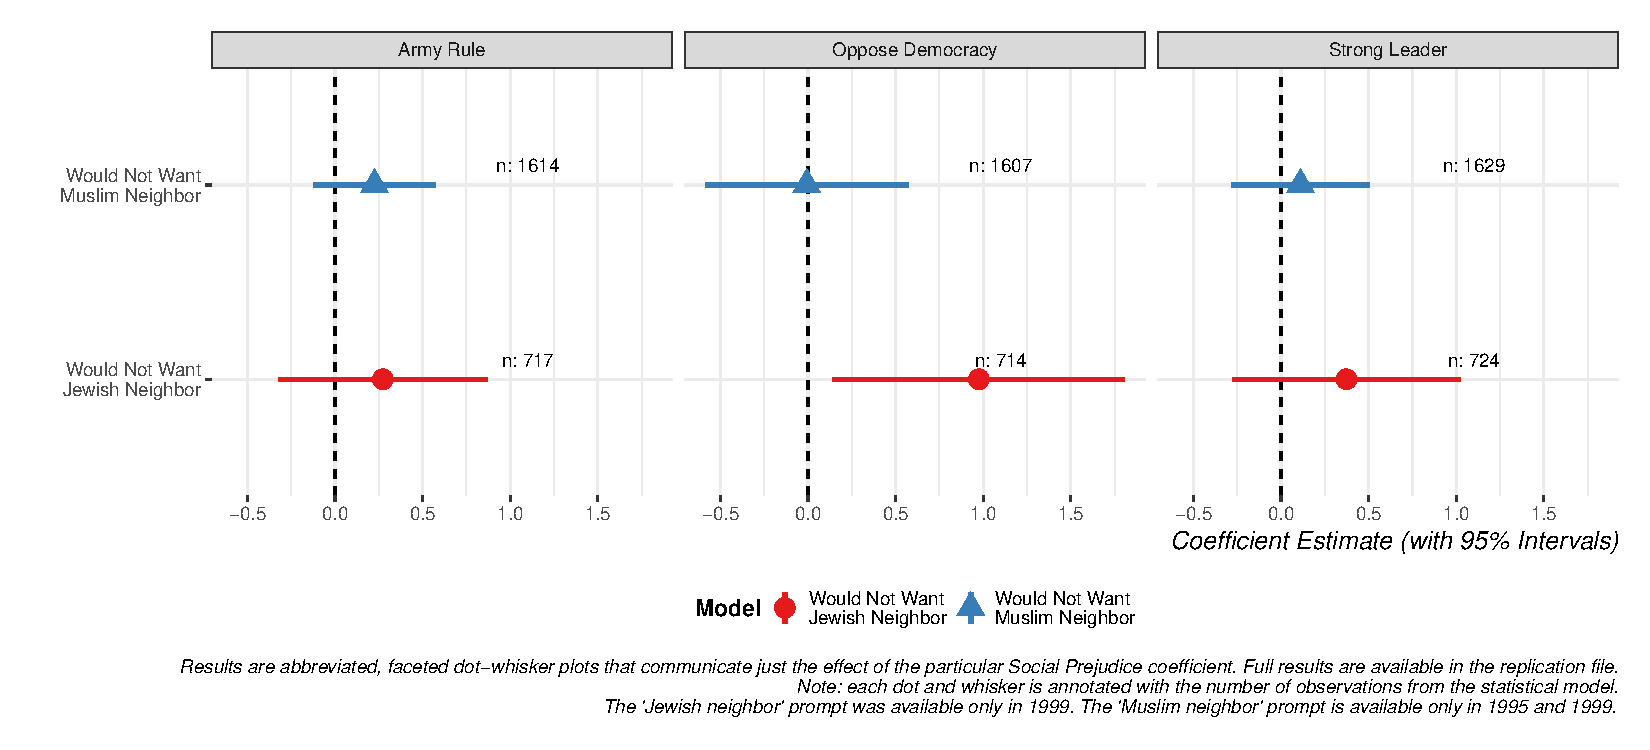
\includegraphics{figs/jmseps.pdf}
\caption{\label{fig:jmseps}Abbreviated Dot-and-Whisker Plots of the
Effect of Prejudice Toward Jews and Muslims on Anti-Democratic
Orientations}
\end{figure}

We also consider whether the ``militant minority'' option affects our
inferences. We can see the intuition behind this response for the sake
of our argument. ``Militant minority'' could easily prime a respondent
to think of an activist group like the Black Panthers, soliciting an
anti-democratic orientation consistent with our argument. It could also
conjure jihadi terrorists given its lone appearance in the first WVS
wave after the September 11, 2001 terror attacks. However, we fear this
term is biased in the measurement sense. A respondent who selects this
could be prejudiced against the ``minority'' or may be reacting to the
``militant'' magnifier that WVS added. A person could justifiably
conjure an image of a potential neighbor sufficiently ``militarized''
with weaponry in that response and not want that person as a neighbor.
We should be careful as researchers to not view that response as
necessarily indicating prejudice against an ethnic/racial minority.

We re-ran the models from Figure 2 in the manuscript, including
potential responses for ``militant minority'' in the 2006 wave in our
white social prejudice variable. The results we report in Table
\ref{tab:mmmodelstab} are substantively identical to Figure 2 in the
manuscript. This holds even though the effect of the ``militant
minority'' treatment drifts negative, per the individual regressions we
ran and summarize as an abbreviated dot-and-whisker plot in Figure
\ref{fig:mmseps}. Table \ref{tab:mmmodelstab} and Figure
\ref{fig:mmseps} offer important takeaways similar to Table
\ref{tab:jwmodelstab} and Figure \ref{fig:jmseps}. Alternate responses
consistent with white social prejudice do not change our inferences when
we add them to our measure but these alternate responses, by themselves,
have no robust effect on anti-democratic orientations. Figure 3 (in the
manuscript) highlights how the effect of the three categories we
included in our measure are robust as individual indicators in a model,
itself a form of a robustness test for the effect of white social
prejudice on anti-democratic orientations of white Americans.

 
  \providecommand{\huxb}[2]{\arrayrulecolor[RGB]{#1}\global\arrayrulewidth=#2pt}
  \providecommand{\huxvb}[2]{\color[RGB]{#1}\vrule width #2pt}
  \providecommand{\huxtpad}[1]{\rule{0pt}{\baselineskip+#1}}
  \providecommand{\huxbpad}[1]{\rule[-#1]{0pt}{#1}}

\begin{table}[!htbp]
\centering
\begin{threeparttable}
\captionsetup{justification=centering,singlelinecheck=off}
\caption{\label{tab:mmmodelstab}The Covariates of Democratic Orientations of White Americans in the World Values Survey [with 'Militant Minority' Responses] (1995-2011)}
\begin{tabularx}{0.6\textwidth}{p{0.15\textwidth} p{0.15\textwidth} p{0.15\textwidth} p{0.15\textwidth}}


\hhline{>{\huxb{0, 0, 0}{0.8}}->{\huxb{0, 0, 0}{0.8}}->{\huxb{0, 0, 0}{0.8}}->{\huxb{0, 0, 0}{0.8}}-}
\arrayrulecolor{black}

\multicolumn{1}{!{\huxvb{0, 0, 0}{0}}c!{\huxvb{0, 0, 0}{0}}}{\huxtpad{4pt}\centering \huxbpad{4pt}} &
\multicolumn{1}{c!{\huxvb{0, 0, 0}{0}}}{\huxtpad{4pt}\centering \textbf{AM10}\huxbpad{4pt}} &
\multicolumn{1}{c!{\huxvb{0, 0, 0}{0}}}{\huxtpad{4pt}\centering \textbf{AM11}\huxbpad{4pt}} &
\multicolumn{1}{c!{\huxvb{0, 0, 0}{0}}}{\huxtpad{4pt}\centering \textbf{AM12}\huxbpad{4pt}} \tabularnewline[-0.5pt]


\hhline{>{\huxb{255, 255, 255}{0.4}}->{\huxb{0, 0, 0}{0.4}}->{\huxb{0, 0, 0}{0.4}}->{\huxb{0, 0, 0}{0.4}}-}
\arrayrulecolor{black}

\multicolumn{1}{!{\huxvb{0, 0, 0}{0}}c!{\huxvb{0, 0, 0}{0}}}{\huxtpad{4pt}\centering \huxbpad{4pt}} &
\multicolumn{1}{c!{\huxvb{0, 0, 0}{0}}}{\huxtpad{4pt}\centering \textit{Strong}\huxbpad{4pt}} &
\multicolumn{1}{c!{\huxvb{0, 0, 0}{0}}}{\huxtpad{4pt}\centering \textit{Army}\huxbpad{4pt}} &
\multicolumn{1}{c!{\huxvb{0, 0, 0}{0}}}{\huxtpad{4pt}\centering \textit{Oppose}\huxbpad{4pt}} \tabularnewline[-0.5pt]


\hhline{}
\arrayrulecolor{black}

\multicolumn{1}{!{\huxvb{0, 0, 0}{0}}c!{\huxvb{0, 0, 0}{0}}}{\huxtpad{4pt}\centering \huxbpad{4pt}} &
\multicolumn{1}{c!{\huxvb{0, 0, 0}{0}}}{\huxtpad{4pt}\centering \textit{Leader}\huxbpad{4pt}} &
\multicolumn{1}{c!{\huxvb{0, 0, 0}{0}}}{\huxtpad{4pt}\centering \textit{Rule}\huxbpad{4pt}} &
\multicolumn{1}{c!{\huxvb{0, 0, 0}{0}}}{\huxtpad{4pt}\centering \textit{Democracy}\huxbpad{4pt}} \tabularnewline[-0.5pt]


\hhline{>{\huxb{0, 0, 0}{0.4}}->{\huxb{0, 0, 0}{0.4}}->{\huxb{0, 0, 0}{0.4}}->{\huxb{0, 0, 0}{0.4}}-}
\arrayrulecolor{black}

\multicolumn{1}{!{\huxvb{0, 0, 0}{0}}c!{\huxvb{0, 0, 0}{0}}}{\huxtpad{4pt}\centering \huxbpad{4pt}} &
\multicolumn{1}{c!{\huxvb{0, 0, 0}{0}}}{\huxtpad{4pt}\centering \huxbpad{4pt}} &
\multicolumn{1}{c!{\huxvb{0, 0, 0}{0}}}{\huxtpad{4pt}\centering \huxbpad{4pt}} &
\multicolumn{1}{c!{\huxvb{0, 0, 0}{0}}}{\huxtpad{4pt}\centering \huxbpad{4pt}} \tabularnewline[-0.5pt]


\hhline{}
\arrayrulecolor{black}

\multicolumn{1}{!{\huxvb{0, 0, 0}{0}}l!{\huxvb{0, 0, 0}{0}}}{\huxtpad{4pt}\raggedright Age\huxbpad{4pt}} &
\multicolumn{1}{c!{\huxvb{0, 0, 0}{0}}}{\huxtpad{4pt}\centering -0.441 ***\huxbpad{4pt}} &
\multicolumn{1}{c!{\huxvb{0, 0, 0}{0}}}{\huxtpad{4pt}\centering -0.449 ***\huxbpad{4pt}} &
\multicolumn{1}{c!{\huxvb{0, 0, 0}{0}}}{\huxtpad{4pt}\centering -0.634 ***\huxbpad{4pt}} \tabularnewline[-0.5pt]


\hhline{}
\arrayrulecolor{black}

\multicolumn{1}{!{\huxvb{0, 0, 0}{0}}l!{\huxvb{0, 0, 0}{0}}}{\huxtpad{4pt}\raggedright \huxbpad{4pt}} &
\multicolumn{1}{c!{\huxvb{0, 0, 0}{0}}}{\huxtpad{4pt}\centering (0.087)\huxbpad{4pt}} &
\multicolumn{1}{c!{\huxvb{0, 0, 0}{0}}}{\huxtpad{4pt}\centering (0.077)\huxbpad{4pt}} &
\multicolumn{1}{c!{\huxvb{0, 0, 0}{0}}}{\huxtpad{4pt}\centering (0.120)\huxbpad{4pt}} \tabularnewline[-0.5pt]


\hhline{}
\arrayrulecolor{black}

\multicolumn{1}{!{\huxvb{0, 0, 0}{0}}l!{\huxvb{0, 0, 0}{0}}}{\huxtpad{4pt}\raggedright Age\verb|^|2\huxbpad{4pt}} &
\multicolumn{1}{c!{\huxvb{0, 0, 0}{0}}}{\huxtpad{4pt}\centering 0.161\huxbpad{4pt}} &
\multicolumn{1}{c!{\huxvb{0, 0, 0}{0}}}{\huxtpad{4pt}\centering 0.045\huxbpad{4pt}} &
\multicolumn{1}{c!{\huxvb{0, 0, 0}{0}}}{\huxtpad{4pt}\centering 0.071\huxbpad{4pt}} \tabularnewline[-0.5pt]


\hhline{}
\arrayrulecolor{black}

\multicolumn{1}{!{\huxvb{0, 0, 0}{0}}l!{\huxvb{0, 0, 0}{0}}}{\huxtpad{4pt}\raggedright \huxbpad{4pt}} &
\multicolumn{1}{c!{\huxvb{0, 0, 0}{0}}}{\huxtpad{4pt}\centering (0.158)\huxbpad{4pt}} &
\multicolumn{1}{c!{\huxvb{0, 0, 0}{0}}}{\huxtpad{4pt}\centering (0.139)\huxbpad{4pt}} &
\multicolumn{1}{c!{\huxvb{0, 0, 0}{0}}}{\huxtpad{4pt}\centering (0.224)\huxbpad{4pt}} \tabularnewline[-0.5pt]


\hhline{}
\arrayrulecolor{black}

\multicolumn{1}{!{\huxvb{0, 0, 0}{0}}l!{\huxvb{0, 0, 0}{0}}}{\huxtpad{4pt}\raggedright Female\huxbpad{4pt}} &
\multicolumn{1}{c!{\huxvb{0, 0, 0}{0}}}{\huxtpad{4pt}\centering 0.041\huxbpad{4pt}} &
\multicolumn{1}{c!{\huxvb{0, 0, 0}{0}}}{\huxtpad{4pt}\centering 0.133\huxbpad{4pt}} &
\multicolumn{1}{c!{\huxvb{0, 0, 0}{0}}}{\huxtpad{4pt}\centering 0.514 ***\huxbpad{4pt}} \tabularnewline[-0.5pt]


\hhline{}
\arrayrulecolor{black}

\multicolumn{1}{!{\huxvb{0, 0, 0}{0}}l!{\huxvb{0, 0, 0}{0}}}{\huxtpad{4pt}\raggedright \huxbpad{4pt}} &
\multicolumn{1}{c!{\huxvb{0, 0, 0}{0}}}{\huxtpad{4pt}\centering (0.084)\huxbpad{4pt}} &
\multicolumn{1}{c!{\huxvb{0, 0, 0}{0}}}{\huxtpad{4pt}\centering (0.072)\huxbpad{4pt}} &
\multicolumn{1}{c!{\huxvb{0, 0, 0}{0}}}{\huxtpad{4pt}\centering (0.118)\huxbpad{4pt}} \tabularnewline[-0.5pt]


\hhline{}
\arrayrulecolor{black}

\multicolumn{1}{!{\huxvb{0, 0, 0}{0}}l!{\huxvb{0, 0, 0}{0}}}{\huxtpad{4pt}\raggedright College Educated\huxbpad{4pt}} &
\multicolumn{1}{c!{\huxvb{0, 0, 0}{0}}}{\huxtpad{4pt}\centering -0.572 ***\huxbpad{4pt}} &
\multicolumn{1}{c!{\huxvb{0, 0, 0}{0}}}{\huxtpad{4pt}\centering -0.162\huxbpad{4pt}} &
\multicolumn{1}{c!{\huxvb{0, 0, 0}{0}}}{\huxtpad{4pt}\centering -1.043 ***\huxbpad{4pt}} \tabularnewline[-0.5pt]


\hhline{}
\arrayrulecolor{black}

\multicolumn{1}{!{\huxvb{0, 0, 0}{0}}l!{\huxvb{0, 0, 0}{0}}}{\huxtpad{4pt}\raggedright \huxbpad{4pt}} &
\multicolumn{1}{c!{\huxvb{0, 0, 0}{0}}}{\huxtpad{4pt}\centering (0.103)\huxbpad{4pt}} &
\multicolumn{1}{c!{\huxvb{0, 0, 0}{0}}}{\huxtpad{4pt}\centering (0.083)\huxbpad{4pt}} &
\multicolumn{1}{c!{\huxvb{0, 0, 0}{0}}}{\huxtpad{4pt}\centering (0.171)\huxbpad{4pt}} \tabularnewline[-0.5pt]


\hhline{}
\arrayrulecolor{black}

\multicolumn{1}{!{\huxvb{0, 0, 0}{0}}l!{\huxvb{0, 0, 0}{0}}}{\huxtpad{4pt}\raggedright Ideology\huxbpad{4pt}} &
\multicolumn{1}{c!{\huxvb{0, 0, 0}{0}}}{\huxtpad{4pt}\centering 0.001\huxbpad{4pt}} &
\multicolumn{1}{c!{\huxvb{0, 0, 0}{0}}}{\huxtpad{4pt}\centering -0.164 *\huxbpad{4pt}} &
\multicolumn{1}{c!{\huxvb{0, 0, 0}{0}}}{\huxtpad{4pt}\centering -0.262\huxbpad{4pt}} \tabularnewline[-0.5pt]


\hhline{}
\arrayrulecolor{black}

\multicolumn{1}{!{\huxvb{0, 0, 0}{0}}l!{\huxvb{0, 0, 0}{0}}}{\huxtpad{4pt}\raggedright \huxbpad{4pt}} &
\multicolumn{1}{c!{\huxvb{0, 0, 0}{0}}}{\huxtpad{4pt}\centering (0.102)\huxbpad{4pt}} &
\multicolumn{1}{c!{\huxvb{0, 0, 0}{0}}}{\huxtpad{4pt}\centering (0.082)\huxbpad{4pt}} &
\multicolumn{1}{c!{\huxvb{0, 0, 0}{0}}}{\huxtpad{4pt}\centering (0.138)\huxbpad{4pt}} \tabularnewline[-0.5pt]


\hhline{}
\arrayrulecolor{black}

\multicolumn{1}{!{\huxvb{0, 0, 0}{0}}l!{\huxvb{0, 0, 0}{0}}}{\huxtpad{4pt}\raggedright Ideology\verb|^|2\huxbpad{4pt}} &
\multicolumn{1}{c!{\huxvb{0, 0, 0}{0}}}{\huxtpad{4pt}\centering -0.528 ***\huxbpad{4pt}} &
\multicolumn{1}{c!{\huxvb{0, 0, 0}{0}}}{\huxtpad{4pt}\centering -0.269 **\huxbpad{4pt}} &
\multicolumn{1}{c!{\huxvb{0, 0, 0}{0}}}{\huxtpad{4pt}\centering -0.125\huxbpad{4pt}} \tabularnewline[-0.5pt]


\hhline{}
\arrayrulecolor{black}

\multicolumn{1}{!{\huxvb{0, 0, 0}{0}}l!{\huxvb{0, 0, 0}{0}}}{\huxtpad{4pt}\raggedright \huxbpad{4pt}} &
\multicolumn{1}{c!{\huxvb{0, 0, 0}{0}}}{\huxtpad{4pt}\centering (0.132)\huxbpad{4pt}} &
\multicolumn{1}{c!{\huxvb{0, 0, 0}{0}}}{\huxtpad{4pt}\centering (0.102)\huxbpad{4pt}} &
\multicolumn{1}{c!{\huxvb{0, 0, 0}{0}}}{\huxtpad{4pt}\centering (0.175)\huxbpad{4pt}} \tabularnewline[-0.5pt]


\hhline{}
\arrayrulecolor{black}

\multicolumn{1}{!{\huxvb{0, 0, 0}{0}}l!{\huxvb{0, 0, 0}{0}}}{\huxtpad{4pt}\raggedright Income Scale\huxbpad{4pt}} &
\multicolumn{1}{c!{\huxvb{0, 0, 0}{0}}}{\huxtpad{4pt}\centering 0.043\huxbpad{4pt}} &
\multicolumn{1}{c!{\huxvb{0, 0, 0}{0}}}{\huxtpad{4pt}\centering -0.015\huxbpad{4pt}} &
\multicolumn{1}{c!{\huxvb{0, 0, 0}{0}}}{\huxtpad{4pt}\centering -0.432 ***\huxbpad{4pt}} \tabularnewline[-0.5pt]


\hhline{}
\arrayrulecolor{black}

\multicolumn{1}{!{\huxvb{0, 0, 0}{0}}l!{\huxvb{0, 0, 0}{0}}}{\huxtpad{4pt}\raggedright \huxbpad{4pt}} &
\multicolumn{1}{c!{\huxvb{0, 0, 0}{0}}}{\huxtpad{4pt}\centering (0.092)\huxbpad{4pt}} &
\multicolumn{1}{c!{\huxvb{0, 0, 0}{0}}}{\huxtpad{4pt}\centering (0.079)\huxbpad{4pt}} &
\multicolumn{1}{c!{\huxvb{0, 0, 0}{0}}}{\huxtpad{4pt}\centering (0.128)\huxbpad{4pt}} \tabularnewline[-0.5pt]


\hhline{}
\arrayrulecolor{black}

\multicolumn{1}{!{\huxvb{0, 0, 0}{0}}l!{\huxvb{0, 0, 0}{0}}}{\huxtpad{4pt}\raggedright Republican\huxbpad{4pt}} &
\multicolumn{1}{c!{\huxvb{0, 0, 0}{0}}}{\huxtpad{4pt}\centering -0.386 **\huxbpad{4pt}} &
\multicolumn{1}{c!{\huxvb{0, 0, 0}{0}}}{\huxtpad{4pt}\centering -0.205\huxbpad{4pt}} &
\multicolumn{1}{c!{\huxvb{0, 0, 0}{0}}}{\huxtpad{4pt}\centering -0.215\huxbpad{4pt}} \tabularnewline[-0.5pt]


\hhline{}
\arrayrulecolor{black}

\multicolumn{1}{!{\huxvb{0, 0, 0}{0}}l!{\huxvb{0, 0, 0}{0}}}{\huxtpad{4pt}\raggedright \huxbpad{4pt}} &
\multicolumn{1}{c!{\huxvb{0, 0, 0}{0}}}{\huxtpad{4pt}\centering (0.130)\huxbpad{4pt}} &
\multicolumn{1}{c!{\huxvb{0, 0, 0}{0}}}{\huxtpad{4pt}\centering (0.115)\huxbpad{4pt}} &
\multicolumn{1}{c!{\huxvb{0, 0, 0}{0}}}{\huxtpad{4pt}\centering (0.159)\huxbpad{4pt}} \tabularnewline[-0.5pt]


\hhline{}
\arrayrulecolor{black}

\multicolumn{1}{!{\huxvb{0, 0, 0}{0}}l!{\huxvb{0, 0, 0}{0}}}{\huxtpad{4pt}\raggedright Democrat\huxbpad{4pt}} &
\multicolumn{1}{c!{\huxvb{0, 0, 0}{0}}}{\huxtpad{4pt}\centering -0.083\huxbpad{4pt}} &
\multicolumn{1}{c!{\huxvb{0, 0, 0}{0}}}{\huxtpad{4pt}\centering -0.064\huxbpad{4pt}} &
\multicolumn{1}{c!{\huxvb{0, 0, 0}{0}}}{\huxtpad{4pt}\centering -1.577 ***\huxbpad{4pt}} \tabularnewline[-0.5pt]


\hhline{}
\arrayrulecolor{black}

\multicolumn{1}{!{\huxvb{0, 0, 0}{0}}l!{\huxvb{0, 0, 0}{0}}}{\huxtpad{4pt}\raggedright \huxbpad{4pt}} &
\multicolumn{1}{c!{\huxvb{0, 0, 0}{0}}}{\huxtpad{4pt}\centering (0.124)\huxbpad{4pt}} &
\multicolumn{1}{c!{\huxvb{0, 0, 0}{0}}}{\huxtpad{4pt}\centering (0.111)\huxbpad{4pt}} &
\multicolumn{1}{c!{\huxvb{0, 0, 0}{0}}}{\huxtpad{4pt}\centering (0.187)\huxbpad{4pt}} \tabularnewline[-0.5pt]


\hhline{}
\arrayrulecolor{black}

\multicolumn{1}{!{\huxvb{0, 0, 0}{0}}l!{\huxvb{0, 0, 0}{0}}}{\huxtpad{4pt}\raggedright Unemployed\huxbpad{4pt}} &
\multicolumn{1}{c!{\huxvb{0, 0, 0}{0}}}{\huxtpad{4pt}\centering 0.530 **\huxbpad{4pt}} &
\multicolumn{1}{c!{\huxvb{0, 0, 0}{0}}}{\huxtpad{4pt}\centering 0.081\huxbpad{4pt}} &
\multicolumn{1}{c!{\huxvb{0, 0, 0}{0}}}{\huxtpad{4pt}\centering 0.608 *\huxbpad{4pt}} \tabularnewline[-0.5pt]


\hhline{}
\arrayrulecolor{black}

\multicolumn{1}{!{\huxvb{0, 0, 0}{0}}l!{\huxvb{0, 0, 0}{0}}}{\huxtpad{4pt}\raggedright \huxbpad{4pt}} &
\multicolumn{1}{c!{\huxvb{0, 0, 0}{0}}}{\huxtpad{4pt}\centering (0.188)\huxbpad{4pt}} &
\multicolumn{1}{c!{\huxvb{0, 0, 0}{0}}}{\huxtpad{4pt}\centering (0.176)\huxbpad{4pt}} &
\multicolumn{1}{c!{\huxvb{0, 0, 0}{0}}}{\huxtpad{4pt}\centering (0.241)\huxbpad{4pt}} \tabularnewline[-0.5pt]


\hhline{}
\arrayrulecolor{black}

\multicolumn{1}{!{\huxvb{0, 0, 0}{0}}l!{\huxvb{0, 0, 0}{0}}}{\huxtpad{4pt}\raggedright Emancipative Values\huxbpad{4pt}} &
\multicolumn{1}{c!{\huxvb{0, 0, 0}{0}}}{\huxtpad{4pt}\centering -0.641 ***\huxbpad{4pt}} &
\multicolumn{1}{c!{\huxvb{0, 0, 0}{0}}}{\huxtpad{4pt}\centering 0.014\huxbpad{4pt}} &
\multicolumn{1}{c!{\huxvb{0, 0, 0}{0}}}{\huxtpad{4pt}\centering -0.700 ***\huxbpad{4pt}} \tabularnewline[-0.5pt]


\hhline{}
\arrayrulecolor{black}

\multicolumn{1}{!{\huxvb{0, 0, 0}{0}}l!{\huxvb{0, 0, 0}{0}}}{\huxtpad{4pt}\raggedright \huxbpad{4pt}} &
\multicolumn{1}{c!{\huxvb{0, 0, 0}{0}}}{\huxtpad{4pt}\centering (0.095)\huxbpad{4pt}} &
\multicolumn{1}{c!{\huxvb{0, 0, 0}{0}}}{\huxtpad{4pt}\centering (0.080)\huxbpad{4pt}} &
\multicolumn{1}{c!{\huxvb{0, 0, 0}{0}}}{\huxtpad{4pt}\centering (0.135)\huxbpad{4pt}} \tabularnewline[-0.5pt]


\hhline{}
\arrayrulecolor{black}

\multicolumn{1}{!{\huxvb{0, 0, 0}{0}}l!{\huxvb{0, 0, 0}{0}}}{\huxtpad{4pt}\raggedright White Social Prejudice\huxbpad{4pt}} &
\multicolumn{1}{c!{\huxvb{0, 0, 0}{0}}}{\huxtpad{4pt}\centering 0.416 ***\huxbpad{4pt}} &
\multicolumn{1}{c!{\huxvb{0, 0, 0}{0}}}{\huxtpad{4pt}\centering 0.314 ***\huxbpad{4pt}} &
\multicolumn{1}{c!{\huxvb{0, 0, 0}{0}}}{\huxtpad{4pt}\centering 0.332 *\huxbpad{4pt}} \tabularnewline[-0.5pt]


\hhline{}
\arrayrulecolor{black}

\multicolumn{1}{!{\huxvb{0, 0, 0}{0}}l!{\huxvb{0, 0, 0}{0}}}{\huxtpad{4pt}\raggedright {\fontsize{7pt}{8.4pt}\selectfont (w/ anti-'Militant Minority' Responses)}\huxbpad{4pt}} &
\multicolumn{1}{c!{\huxvb{0, 0, 0}{0}}}{\huxtpad{4pt}\centering (0.099)\huxbpad{4pt}} &
\multicolumn{1}{c!{\huxvb{0, 0, 0}{0}}}{\huxtpad{4pt}\centering (0.089)\huxbpad{4pt}} &
\multicolumn{1}{c!{\huxvb{0, 0, 0}{0}}}{\huxtpad{4pt}\centering (0.134)\huxbpad{4pt}} \tabularnewline[-0.5pt]


\hhline{}
\arrayrulecolor{black}

\multicolumn{1}{!{\huxvb{0, 0, 0}{0}}l!{\huxvb{0, 0, 0}{0}}}{\huxtpad{4pt}\raggedright \huxbpad{4pt}} &
\multicolumn{1}{c!{\huxvb{0, 0, 0}{0}}}{\huxtpad{4pt}\centering \huxbpad{4pt}} &
\multicolumn{1}{c!{\huxvb{0, 0, 0}{0}}}{\huxtpad{4pt}\centering \huxbpad{4pt}} &
\multicolumn{1}{c!{\huxvb{0, 0, 0}{0}}}{\huxtpad{4pt}\centering \huxbpad{4pt}} \tabularnewline[-0.5pt]


\hhline{}
\arrayrulecolor{black}

\multicolumn{1}{!{\huxvb{0, 0, 0}{0}}l!{\huxvb{0, 0, 0}{0}}}{\huxtpad{4pt}\raggedright \textit{Random Effect}\huxbpad{4pt}} &
\multicolumn{1}{c!{\huxvb{0, 0, 0}{0}}}{\huxtpad{4pt}\centering \huxbpad{4pt}} &
\multicolumn{1}{c!{\huxvb{0, 0, 0}{0}}}{\huxtpad{4pt}\centering \huxbpad{4pt}} &
\multicolumn{1}{c!{\huxvb{0, 0, 0}{0}}}{\huxtpad{4pt}\centering \huxbpad{4pt}} \tabularnewline[-0.5pt]


\hhline{}
\arrayrulecolor{black}

\multicolumn{1}{!{\huxvb{0, 0, 0}{0}}l!{\huxvb{0, 0, 0}{0}}}{\huxtpad{4pt}\raggedright sd(Year)\huxbpad{4pt}} &
\multicolumn{1}{c!{\huxvb{0, 0, 0}{0}}}{\huxtpad{4pt}\centering 0.168\huxbpad{4pt}} &
\multicolumn{1}{c!{\huxvb{0, 0, 0}{0}}}{\huxtpad{4pt}\centering 0.219\huxbpad{4pt}} &
\multicolumn{1}{c!{\huxvb{0, 0, 0}{0}}}{\huxtpad{4pt}\centering 0.228\huxbpad{4pt}} \tabularnewline[-0.5pt]


\hhline{}
\arrayrulecolor{black}

\multicolumn{1}{!{\huxvb{0, 0, 0}{0}}l!{\huxvb{0, 0, 0}{0}}}{\huxtpad{4pt}\raggedright \huxbpad{4pt}} &
\multicolumn{1}{c!{\huxvb{0, 0, 0}{0}}}{\huxtpad{4pt}\centering \huxbpad{4pt}} &
\multicolumn{1}{c!{\huxvb{0, 0, 0}{0}}}{\huxtpad{4pt}\centering \huxbpad{4pt}} &
\multicolumn{1}{c!{\huxvb{0, 0, 0}{0}}}{\huxtpad{4pt}\centering \huxbpad{4pt}} \tabularnewline[-0.5pt]


\hhline{}
\arrayrulecolor{black}

\multicolumn{1}{!{\huxvb{0, 0, 0}{0}}l!{\huxvb{0, 0, 0}{0}}}{\huxtpad{4pt}\raggedright N\huxbpad{4pt}} &
\multicolumn{1}{c!{\huxvb{0, 0, 0}{0}}}{\huxtpad{4pt}\centering 3452\huxbpad{4pt}} &
\multicolumn{1}{c!{\huxvb{0, 0, 0}{0}}}{\huxtpad{4pt}\centering 3433\huxbpad{4pt}} &
\multicolumn{1}{c!{\huxvb{0, 0, 0}{0}}}{\huxtpad{4pt}\centering 3421\huxbpad{4pt}} \tabularnewline[-0.5pt]


\hhline{>{\huxb{0, 0, 0}{0.8}}->{\huxb{0, 0, 0}{0.8}}->{\huxb{0, 0, 0}{0.8}}->{\huxb{0, 0, 0}{0.8}}-}
\arrayrulecolor{black}

\multicolumn{4}{!{\huxvb{0, 0, 0}{0}}p{0.6\textwidth+6\tabcolsep}!{\huxvb{0, 0, 0}{0}}}{\parbox[b]{0.6\textwidth+6\tabcolsep-4pt-4pt}{\huxtpad{4pt}\raggedright  *** p $<$ 0.001;  ** p $<$ 0.01;  * p $<$ 0.05.\huxbpad{4pt}}} \tabularnewline[-0.5pt]


\hhline{}
\arrayrulecolor{black}
\end{tabularx}\end{threeparttable}


\end{table}
 

\begin{figure}
\centering
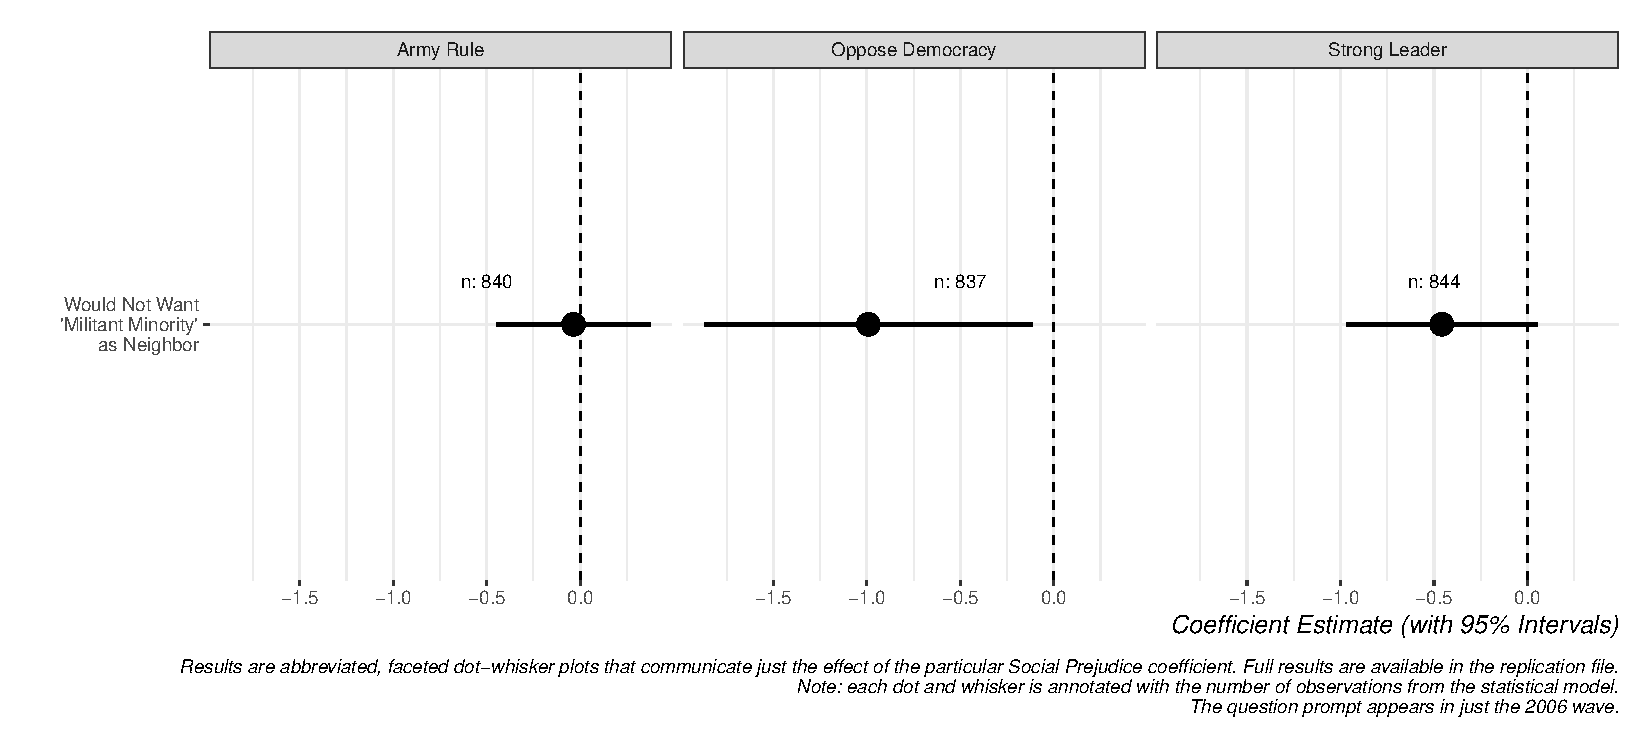
\includegraphics{figs/mmseps.pdf}
\caption{\label{fig:mmseps}Abbreviated Dot-and-Whisker Plots of the
Effect of Not Wanting a `Militant Minority' for a Neighbor on
Anti-Democratic Orientations}
\end{figure}

We do a similar estimation approach that looks at the effect of
anti-LGBT responses captured in the ``homosexuals'' item. Anti-LGBT
prejudice has been a recurring theme in the Ku Klux Klan \citep[for
example]{gibson1987hkkk} and it is not uncommon for white people who
espouse prejudice toward members of a difference race or immigrants to
also espouse prejudice toward LGBT individuals. We develop two means to
explore the effect of anti-LGBT prejudice on anti-democratic
orientations. First, we code a 1 for any respondent who would not want a
homosexual (per the item prompt) as a neighbor in addition to any of the
three main items we code as part of our prejudice measure. Further, we
look at the effect of this item in particular on anti-democratic
orientations.

 
  \providecommand{\huxb}[2]{\arrayrulecolor[RGB]{#1}\global\arrayrulewidth=#2pt}
  \providecommand{\huxvb}[2]{\color[RGB]{#1}\vrule width #2pt}
  \providecommand{\huxtpad}[1]{\rule{0pt}{\baselineskip+#1}}
  \providecommand{\huxbpad}[1]{\rule[-#1]{0pt}{#1}}

\begin{table}[!htbp]
\centering
\begin{threeparttable}
\captionsetup{justification=centering,singlelinecheck=off}
\caption{\label{tab:lgbtmodelstab}The Covariates of Democratic Orientations of White Americans in the World Values Survey [with anti-LGBT Responses] (1995-2011)}
\begin{tabularx}{0.6\textwidth}{p{0.15\textwidth} p{0.15\textwidth} p{0.15\textwidth} p{0.15\textwidth}}


\hhline{>{\huxb{0, 0, 0}{0.8}}->{\huxb{0, 0, 0}{0.8}}->{\huxb{0, 0, 0}{0.8}}->{\huxb{0, 0, 0}{0.8}}-}
\arrayrulecolor{black}

\multicolumn{1}{!{\huxvb{0, 0, 0}{0}}c!{\huxvb{0, 0, 0}{0}}}{\huxtpad{4pt}\centering \huxbpad{4pt}} &
\multicolumn{1}{c!{\huxvb{0, 0, 0}{0}}}{\huxtpad{4pt}\centering \textbf{AM7}\huxbpad{4pt}} &
\multicolumn{1}{c!{\huxvb{0, 0, 0}{0}}}{\huxtpad{4pt}\centering \textbf{AM8}\huxbpad{4pt}} &
\multicolumn{1}{c!{\huxvb{0, 0, 0}{0}}}{\huxtpad{4pt}\centering \textbf{AM9}\huxbpad{4pt}} \tabularnewline[-0.5pt]


\hhline{>{\huxb{255, 255, 255}{0.4}}->{\huxb{0, 0, 0}{0.4}}->{\huxb{0, 0, 0}{0.4}}->{\huxb{0, 0, 0}{0.4}}-}
\arrayrulecolor{black}

\multicolumn{1}{!{\huxvb{0, 0, 0}{0}}c!{\huxvb{0, 0, 0}{0}}}{\huxtpad{4pt}\centering \huxbpad{4pt}} &
\multicolumn{1}{c!{\huxvb{0, 0, 0}{0}}}{\huxtpad{4pt}\centering \textit{Strong}\huxbpad{4pt}} &
\multicolumn{1}{c!{\huxvb{0, 0, 0}{0}}}{\huxtpad{4pt}\centering \textit{Army}\huxbpad{4pt}} &
\multicolumn{1}{c!{\huxvb{0, 0, 0}{0}}}{\huxtpad{4pt}\centering \textit{Oppose}\huxbpad{4pt}} \tabularnewline[-0.5pt]


\hhline{}
\arrayrulecolor{black}

\multicolumn{1}{!{\huxvb{0, 0, 0}{0}}c!{\huxvb{0, 0, 0}{0}}}{\huxtpad{4pt}\centering \huxbpad{4pt}} &
\multicolumn{1}{c!{\huxvb{0, 0, 0}{0}}}{\huxtpad{4pt}\centering \textit{Leader}\huxbpad{4pt}} &
\multicolumn{1}{c!{\huxvb{0, 0, 0}{0}}}{\huxtpad{4pt}\centering \textit{Rule}\huxbpad{4pt}} &
\multicolumn{1}{c!{\huxvb{0, 0, 0}{0}}}{\huxtpad{4pt}\centering \textit{Democracy}\huxbpad{4pt}} \tabularnewline[-0.5pt]


\hhline{>{\huxb{0, 0, 0}{0.4}}->{\huxb{0, 0, 0}{0.4}}->{\huxb{0, 0, 0}{0.4}}->{\huxb{0, 0, 0}{0.4}}-}
\arrayrulecolor{black}

\multicolumn{1}{!{\huxvb{0, 0, 0}{0}}c!{\huxvb{0, 0, 0}{0}}}{\huxtpad{4pt}\centering \huxbpad{4pt}} &
\multicolumn{1}{c!{\huxvb{0, 0, 0}{0}}}{\huxtpad{4pt}\centering \huxbpad{4pt}} &
\multicolumn{1}{c!{\huxvb{0, 0, 0}{0}}}{\huxtpad{4pt}\centering \huxbpad{4pt}} &
\multicolumn{1}{c!{\huxvb{0, 0, 0}{0}}}{\huxtpad{4pt}\centering \huxbpad{4pt}} \tabularnewline[-0.5pt]


\hhline{}
\arrayrulecolor{black}

\multicolumn{1}{!{\huxvb{0, 0, 0}{0}}l!{\huxvb{0, 0, 0}{0}}}{\huxtpad{4pt}\raggedright Age\huxbpad{4pt}} &
\multicolumn{1}{c!{\huxvb{0, 0, 0}{0}}}{\huxtpad{4pt}\centering -0.450 ***\huxbpad{4pt}} &
\multicolumn{1}{c!{\huxvb{0, 0, 0}{0}}}{\huxtpad{4pt}\centering -0.454 ***\huxbpad{4pt}} &
\multicolumn{1}{c!{\huxvb{0, 0, 0}{0}}}{\huxtpad{4pt}\centering -0.641 ***\huxbpad{4pt}} \tabularnewline[-0.5pt]


\hhline{}
\arrayrulecolor{black}

\multicolumn{1}{!{\huxvb{0, 0, 0}{0}}l!{\huxvb{0, 0, 0}{0}}}{\huxtpad{4pt}\raggedright \huxbpad{4pt}} &
\multicolumn{1}{c!{\huxvb{0, 0, 0}{0}}}{\huxtpad{4pt}\centering (0.087)\huxbpad{4pt}} &
\multicolumn{1}{c!{\huxvb{0, 0, 0}{0}}}{\huxtpad{4pt}\centering (0.077)\huxbpad{4pt}} &
\multicolumn{1}{c!{\huxvb{0, 0, 0}{0}}}{\huxtpad{4pt}\centering (0.120)\huxbpad{4pt}} \tabularnewline[-0.5pt]


\hhline{}
\arrayrulecolor{black}

\multicolumn{1}{!{\huxvb{0, 0, 0}{0}}l!{\huxvb{0, 0, 0}{0}}}{\huxtpad{4pt}\raggedright Age\verb|^|2\huxbpad{4pt}} &
\multicolumn{1}{c!{\huxvb{0, 0, 0}{0}}}{\huxtpad{4pt}\centering 0.149\huxbpad{4pt}} &
\multicolumn{1}{c!{\huxvb{0, 0, 0}{0}}}{\huxtpad{4pt}\centering 0.037\huxbpad{4pt}} &
\multicolumn{1}{c!{\huxvb{0, 0, 0}{0}}}{\huxtpad{4pt}\centering 0.062\huxbpad{4pt}} \tabularnewline[-0.5pt]


\hhline{}
\arrayrulecolor{black}

\multicolumn{1}{!{\huxvb{0, 0, 0}{0}}l!{\huxvb{0, 0, 0}{0}}}{\huxtpad{4pt}\raggedright \huxbpad{4pt}} &
\multicolumn{1}{c!{\huxvb{0, 0, 0}{0}}}{\huxtpad{4pt}\centering (0.158)\huxbpad{4pt}} &
\multicolumn{1}{c!{\huxvb{0, 0, 0}{0}}}{\huxtpad{4pt}\centering (0.139)\huxbpad{4pt}} &
\multicolumn{1}{c!{\huxvb{0, 0, 0}{0}}}{\huxtpad{4pt}\centering (0.223)\huxbpad{4pt}} \tabularnewline[-0.5pt]


\hhline{}
\arrayrulecolor{black}

\multicolumn{1}{!{\huxvb{0, 0, 0}{0}}l!{\huxvb{0, 0, 0}{0}}}{\huxtpad{4pt}\raggedright Female\huxbpad{4pt}} &
\multicolumn{1}{c!{\huxvb{0, 0, 0}{0}}}{\huxtpad{4pt}\centering 0.060\huxbpad{4pt}} &
\multicolumn{1}{c!{\huxvb{0, 0, 0}{0}}}{\huxtpad{4pt}\centering 0.145 *\huxbpad{4pt}} &
\multicolumn{1}{c!{\huxvb{0, 0, 0}{0}}}{\huxtpad{4pt}\centering 0.533 ***\huxbpad{4pt}} \tabularnewline[-0.5pt]


\hhline{}
\arrayrulecolor{black}

\multicolumn{1}{!{\huxvb{0, 0, 0}{0}}l!{\huxvb{0, 0, 0}{0}}}{\huxtpad{4pt}\raggedright \huxbpad{4pt}} &
\multicolumn{1}{c!{\huxvb{0, 0, 0}{0}}}{\huxtpad{4pt}\centering (0.084)\huxbpad{4pt}} &
\multicolumn{1}{c!{\huxvb{0, 0, 0}{0}}}{\huxtpad{4pt}\centering (0.072)\huxbpad{4pt}} &
\multicolumn{1}{c!{\huxvb{0, 0, 0}{0}}}{\huxtpad{4pt}\centering (0.119)\huxbpad{4pt}} \tabularnewline[-0.5pt]


\hhline{}
\arrayrulecolor{black}

\multicolumn{1}{!{\huxvb{0, 0, 0}{0}}l!{\huxvb{0, 0, 0}{0}}}{\huxtpad{4pt}\raggedright College Educated\huxbpad{4pt}} &
\multicolumn{1}{c!{\huxvb{0, 0, 0}{0}}}{\huxtpad{4pt}\centering -0.568 ***\huxbpad{4pt}} &
\multicolumn{1}{c!{\huxvb{0, 0, 0}{0}}}{\huxtpad{4pt}\centering -0.159\huxbpad{4pt}} &
\multicolumn{1}{c!{\huxvb{0, 0, 0}{0}}}{\huxtpad{4pt}\centering -1.034 ***\huxbpad{4pt}} \tabularnewline[-0.5pt]


\hhline{}
\arrayrulecolor{black}

\multicolumn{1}{!{\huxvb{0, 0, 0}{0}}l!{\huxvb{0, 0, 0}{0}}}{\huxtpad{4pt}\raggedright \huxbpad{4pt}} &
\multicolumn{1}{c!{\huxvb{0, 0, 0}{0}}}{\huxtpad{4pt}\centering (0.103)\huxbpad{4pt}} &
\multicolumn{1}{c!{\huxvb{0, 0, 0}{0}}}{\huxtpad{4pt}\centering (0.083)\huxbpad{4pt}} &
\multicolumn{1}{c!{\huxvb{0, 0, 0}{0}}}{\huxtpad{4pt}\centering (0.171)\huxbpad{4pt}} \tabularnewline[-0.5pt]


\hhline{}
\arrayrulecolor{black}

\multicolumn{1}{!{\huxvb{0, 0, 0}{0}}l!{\huxvb{0, 0, 0}{0}}}{\huxtpad{4pt}\raggedright Ideology\huxbpad{4pt}} &
\multicolumn{1}{c!{\huxvb{0, 0, 0}{0}}}{\huxtpad{4pt}\centering -0.006\huxbpad{4pt}} &
\multicolumn{1}{c!{\huxvb{0, 0, 0}{0}}}{\huxtpad{4pt}\centering -0.170 *\huxbpad{4pt}} &
\multicolumn{1}{c!{\huxvb{0, 0, 0}{0}}}{\huxtpad{4pt}\centering -0.267\huxbpad{4pt}} \tabularnewline[-0.5pt]


\hhline{}
\arrayrulecolor{black}

\multicolumn{1}{!{\huxvb{0, 0, 0}{0}}l!{\huxvb{0, 0, 0}{0}}}{\huxtpad{4pt}\raggedright \huxbpad{4pt}} &
\multicolumn{1}{c!{\huxvb{0, 0, 0}{0}}}{\huxtpad{4pt}\centering (0.102)\huxbpad{4pt}} &
\multicolumn{1}{c!{\huxvb{0, 0, 0}{0}}}{\huxtpad{4pt}\centering (0.082)\huxbpad{4pt}} &
\multicolumn{1}{c!{\huxvb{0, 0, 0}{0}}}{\huxtpad{4pt}\centering (0.138)\huxbpad{4pt}} \tabularnewline[-0.5pt]


\hhline{}
\arrayrulecolor{black}

\multicolumn{1}{!{\huxvb{0, 0, 0}{0}}l!{\huxvb{0, 0, 0}{0}}}{\huxtpad{4pt}\raggedright Ideology\verb|^|2\huxbpad{4pt}} &
\multicolumn{1}{c!{\huxvb{0, 0, 0}{0}}}{\huxtpad{4pt}\centering -0.552 ***\huxbpad{4pt}} &
\multicolumn{1}{c!{\huxvb{0, 0, 0}{0}}}{\huxtpad{4pt}\centering -0.287 **\huxbpad{4pt}} &
\multicolumn{1}{c!{\huxvb{0, 0, 0}{0}}}{\huxtpad{4pt}\centering -0.152\huxbpad{4pt}} \tabularnewline[-0.5pt]


\hhline{}
\arrayrulecolor{black}

\multicolumn{1}{!{\huxvb{0, 0, 0}{0}}l!{\huxvb{0, 0, 0}{0}}}{\huxtpad{4pt}\raggedright \huxbpad{4pt}} &
\multicolumn{1}{c!{\huxvb{0, 0, 0}{0}}}{\huxtpad{4pt}\centering (0.132)\huxbpad{4pt}} &
\multicolumn{1}{c!{\huxvb{0, 0, 0}{0}}}{\huxtpad{4pt}\centering (0.102)\huxbpad{4pt}} &
\multicolumn{1}{c!{\huxvb{0, 0, 0}{0}}}{\huxtpad{4pt}\centering (0.176)\huxbpad{4pt}} \tabularnewline[-0.5pt]


\hhline{}
\arrayrulecolor{black}

\multicolumn{1}{!{\huxvb{0, 0, 0}{0}}l!{\huxvb{0, 0, 0}{0}}}{\huxtpad{4pt}\raggedright Income Scale\huxbpad{4pt}} &
\multicolumn{1}{c!{\huxvb{0, 0, 0}{0}}}{\huxtpad{4pt}\centering 0.052\huxbpad{4pt}} &
\multicolumn{1}{c!{\huxvb{0, 0, 0}{0}}}{\huxtpad{4pt}\centering -0.009\huxbpad{4pt}} &
\multicolumn{1}{c!{\huxvb{0, 0, 0}{0}}}{\huxtpad{4pt}\centering -0.430 ***\huxbpad{4pt}} \tabularnewline[-0.5pt]


\hhline{}
\arrayrulecolor{black}

\multicolumn{1}{!{\huxvb{0, 0, 0}{0}}l!{\huxvb{0, 0, 0}{0}}}{\huxtpad{4pt}\raggedright \huxbpad{4pt}} &
\multicolumn{1}{c!{\huxvb{0, 0, 0}{0}}}{\huxtpad{4pt}\centering (0.092)\huxbpad{4pt}} &
\multicolumn{1}{c!{\huxvb{0, 0, 0}{0}}}{\huxtpad{4pt}\centering (0.079)\huxbpad{4pt}} &
\multicolumn{1}{c!{\huxvb{0, 0, 0}{0}}}{\huxtpad{4pt}\centering (0.128)\huxbpad{4pt}} \tabularnewline[-0.5pt]


\hhline{}
\arrayrulecolor{black}

\multicolumn{1}{!{\huxvb{0, 0, 0}{0}}l!{\huxvb{0, 0, 0}{0}}}{\huxtpad{4pt}\raggedright Republican\huxbpad{4pt}} &
\multicolumn{1}{c!{\huxvb{0, 0, 0}{0}}}{\huxtpad{4pt}\centering -0.406 **\huxbpad{4pt}} &
\multicolumn{1}{c!{\huxvb{0, 0, 0}{0}}}{\huxtpad{4pt}\centering -0.217\huxbpad{4pt}} &
\multicolumn{1}{c!{\huxvb{0, 0, 0}{0}}}{\huxtpad{4pt}\centering -0.236\huxbpad{4pt}} \tabularnewline[-0.5pt]


\hhline{}
\arrayrulecolor{black}

\multicolumn{1}{!{\huxvb{0, 0, 0}{0}}l!{\huxvb{0, 0, 0}{0}}}{\huxtpad{4pt}\raggedright \huxbpad{4pt}} &
\multicolumn{1}{c!{\huxvb{0, 0, 0}{0}}}{\huxtpad{4pt}\centering (0.130)\huxbpad{4pt}} &
\multicolumn{1}{c!{\huxvb{0, 0, 0}{0}}}{\huxtpad{4pt}\centering (0.115)\huxbpad{4pt}} &
\multicolumn{1}{c!{\huxvb{0, 0, 0}{0}}}{\huxtpad{4pt}\centering (0.160)\huxbpad{4pt}} \tabularnewline[-0.5pt]


\hhline{}
\arrayrulecolor{black}

\multicolumn{1}{!{\huxvb{0, 0, 0}{0}}l!{\huxvb{0, 0, 0}{0}}}{\huxtpad{4pt}\raggedright Democrat\huxbpad{4pt}} &
\multicolumn{1}{c!{\huxvb{0, 0, 0}{0}}}{\huxtpad{4pt}\centering -0.084\huxbpad{4pt}} &
\multicolumn{1}{c!{\huxvb{0, 0, 0}{0}}}{\huxtpad{4pt}\centering -0.064\huxbpad{4pt}} &
\multicolumn{1}{c!{\huxvb{0, 0, 0}{0}}}{\huxtpad{4pt}\centering -1.576 ***\huxbpad{4pt}} \tabularnewline[-0.5pt]


\hhline{}
\arrayrulecolor{black}

\multicolumn{1}{!{\huxvb{0, 0, 0}{0}}l!{\huxvb{0, 0, 0}{0}}}{\huxtpad{4pt}\raggedright \huxbpad{4pt}} &
\multicolumn{1}{c!{\huxvb{0, 0, 0}{0}}}{\huxtpad{4pt}\centering (0.124)\huxbpad{4pt}} &
\multicolumn{1}{c!{\huxvb{0, 0, 0}{0}}}{\huxtpad{4pt}\centering (0.111)\huxbpad{4pt}} &
\multicolumn{1}{c!{\huxvb{0, 0, 0}{0}}}{\huxtpad{4pt}\centering (0.187)\huxbpad{4pt}} \tabularnewline[-0.5pt]


\hhline{}
\arrayrulecolor{black}

\multicolumn{1}{!{\huxvb{0, 0, 0}{0}}l!{\huxvb{0, 0, 0}{0}}}{\huxtpad{4pt}\raggedright Unemployed\huxbpad{4pt}} &
\multicolumn{1}{c!{\huxvb{0, 0, 0}{0}}}{\huxtpad{4pt}\centering 0.524 **\huxbpad{4pt}} &
\multicolumn{1}{c!{\huxvb{0, 0, 0}{0}}}{\huxtpad{4pt}\centering 0.075\huxbpad{4pt}} &
\multicolumn{1}{c!{\huxvb{0, 0, 0}{0}}}{\huxtpad{4pt}\centering 0.604 *\huxbpad{4pt}} \tabularnewline[-0.5pt]


\hhline{}
\arrayrulecolor{black}

\multicolumn{1}{!{\huxvb{0, 0, 0}{0}}l!{\huxvb{0, 0, 0}{0}}}{\huxtpad{4pt}\raggedright \huxbpad{4pt}} &
\multicolumn{1}{c!{\huxvb{0, 0, 0}{0}}}{\huxtpad{4pt}\centering (0.188)\huxbpad{4pt}} &
\multicolumn{1}{c!{\huxvb{0, 0, 0}{0}}}{\huxtpad{4pt}\centering (0.176)\huxbpad{4pt}} &
\multicolumn{1}{c!{\huxvb{0, 0, 0}{0}}}{\huxtpad{4pt}\centering (0.241)\huxbpad{4pt}} \tabularnewline[-0.5pt]


\hhline{}
\arrayrulecolor{black}

\multicolumn{1}{!{\huxvb{0, 0, 0}{0}}l!{\huxvb{0, 0, 0}{0}}}{\huxtpad{4pt}\raggedright Emancipative Values\huxbpad{4pt}} &
\multicolumn{1}{c!{\huxvb{0, 0, 0}{0}}}{\huxtpad{4pt}\centering -0.565 ***\huxbpad{4pt}} &
\multicolumn{1}{c!{\huxvb{0, 0, 0}{0}}}{\huxtpad{4pt}\centering 0.066\huxbpad{4pt}} &
\multicolumn{1}{c!{\huxvb{0, 0, 0}{0}}}{\huxtpad{4pt}\centering -0.611 ***\huxbpad{4pt}} \tabularnewline[-0.5pt]


\hhline{}
\arrayrulecolor{black}

\multicolumn{1}{!{\huxvb{0, 0, 0}{0}}l!{\huxvb{0, 0, 0}{0}}}{\huxtpad{4pt}\raggedright \huxbpad{4pt}} &
\multicolumn{1}{c!{\huxvb{0, 0, 0}{0}}}{\huxtpad{4pt}\centering (0.097)\huxbpad{4pt}} &
\multicolumn{1}{c!{\huxvb{0, 0, 0}{0}}}{\huxtpad{4pt}\centering (0.082)\huxbpad{4pt}} &
\multicolumn{1}{c!{\huxvb{0, 0, 0}{0}}}{\huxtpad{4pt}\centering (0.138)\huxbpad{4pt}} \tabularnewline[-0.5pt]


\hhline{}
\arrayrulecolor{black}

\multicolumn{1}{!{\huxvb{0, 0, 0}{0}}l!{\huxvb{0, 0, 0}{0}}}{\huxtpad{4pt}\raggedright White Social Prejudice\huxbpad{4pt}} &
\multicolumn{1}{c!{\huxvb{0, 0, 0}{0}}}{\huxtpad{4pt}\centering 0.393 ***\huxbpad{4pt}} &
\multicolumn{1}{c!{\huxvb{0, 0, 0}{0}}}{\huxtpad{4pt}\centering 0.282 ***\huxbpad{4pt}} &
\multicolumn{1}{c!{\huxvb{0, 0, 0}{0}}}{\huxtpad{4pt}\centering 0.415 ***\huxbpad{4pt}} \tabularnewline[-0.5pt]


\hhline{}
\arrayrulecolor{black}

\multicolumn{1}{!{\huxvb{0, 0, 0}{0}}l!{\huxvb{0, 0, 0}{0}}}{\huxtpad{4pt}\raggedright {\fontsize{7pt}{8.4pt}\selectfont (w/ anti-LGBT Responses)}\huxbpad{4pt}} &
\multicolumn{1}{c!{\huxvb{0, 0, 0}{0}}}{\huxtpad{4pt}\centering (0.089)\huxbpad{4pt}} &
\multicolumn{1}{c!{\huxvb{0, 0, 0}{0}}}{\huxtpad{4pt}\centering (0.079)\huxbpad{4pt}} &
\multicolumn{1}{c!{\huxvb{0, 0, 0}{0}}}{\huxtpad{4pt}\centering (0.122)\huxbpad{4pt}} \tabularnewline[-0.5pt]


\hhline{}
\arrayrulecolor{black}

\multicolumn{1}{!{\huxvb{0, 0, 0}{0}}l!{\huxvb{0, 0, 0}{0}}}{\huxtpad{4pt}\raggedright \huxbpad{4pt}} &
\multicolumn{1}{c!{\huxvb{0, 0, 0}{0}}}{\huxtpad{4pt}\centering \huxbpad{4pt}} &
\multicolumn{1}{c!{\huxvb{0, 0, 0}{0}}}{\huxtpad{4pt}\centering \huxbpad{4pt}} &
\multicolumn{1}{c!{\huxvb{0, 0, 0}{0}}}{\huxtpad{4pt}\centering \huxbpad{4pt}} \tabularnewline[-0.5pt]


\hhline{}
\arrayrulecolor{black}

\multicolumn{1}{!{\huxvb{0, 0, 0}{0}}l!{\huxvb{0, 0, 0}{0}}}{\huxtpad{4pt}\raggedright \textit{Random Effect}\huxbpad{4pt}} &
\multicolumn{1}{c!{\huxvb{0, 0, 0}{0}}}{\huxtpad{4pt}\centering \huxbpad{4pt}} &
\multicolumn{1}{c!{\huxvb{0, 0, 0}{0}}}{\huxtpad{4pt}\centering \huxbpad{4pt}} &
\multicolumn{1}{c!{\huxvb{0, 0, 0}{0}}}{\huxtpad{4pt}\centering \huxbpad{4pt}} \tabularnewline[-0.5pt]


\hhline{}
\arrayrulecolor{black}

\multicolumn{1}{!{\huxvb{0, 0, 0}{0}}l!{\huxvb{0, 0, 0}{0}}}{\huxtpad{4pt}\raggedright sd(Year)\huxbpad{4pt}} &
\multicolumn{1}{c!{\huxvb{0, 0, 0}{0}}}{\huxtpad{4pt}\centering 0.199\huxbpad{4pt}} &
\multicolumn{1}{c!{\huxvb{0, 0, 0}{0}}}{\huxtpad{4pt}\centering 0.237\huxbpad{4pt}} &
\multicolumn{1}{c!{\huxvb{0, 0, 0}{0}}}{\huxtpad{4pt}\centering 0.233\huxbpad{4pt}} \tabularnewline[-0.5pt]


\hhline{}
\arrayrulecolor{black}

\multicolumn{1}{!{\huxvb{0, 0, 0}{0}}l!{\huxvb{0, 0, 0}{0}}}{\huxtpad{4pt}\raggedright \huxbpad{4pt}} &
\multicolumn{1}{c!{\huxvb{0, 0, 0}{0}}}{\huxtpad{4pt}\centering \huxbpad{4pt}} &
\multicolumn{1}{c!{\huxvb{0, 0, 0}{0}}}{\huxtpad{4pt}\centering \huxbpad{4pt}} &
\multicolumn{1}{c!{\huxvb{0, 0, 0}{0}}}{\huxtpad{4pt}\centering \huxbpad{4pt}} \tabularnewline[-0.5pt]


\hhline{}
\arrayrulecolor{black}

\multicolumn{1}{!{\huxvb{0, 0, 0}{0}}l!{\huxvb{0, 0, 0}{0}}}{\huxtpad{4pt}\raggedright N\huxbpad{4pt}} &
\multicolumn{1}{c!{\huxvb{0, 0, 0}{0}}}{\huxtpad{4pt}\centering 3452\huxbpad{4pt}} &
\multicolumn{1}{c!{\huxvb{0, 0, 0}{0}}}{\huxtpad{4pt}\centering 3433\huxbpad{4pt}} &
\multicolumn{1}{c!{\huxvb{0, 0, 0}{0}}}{\huxtpad{4pt}\centering 3421\huxbpad{4pt}} \tabularnewline[-0.5pt]


\hhline{>{\huxb{0, 0, 0}{0.8}}->{\huxb{0, 0, 0}{0.8}}->{\huxb{0, 0, 0}{0.8}}->{\huxb{0, 0, 0}{0.8}}-}
\arrayrulecolor{black}

\multicolumn{4}{!{\huxvb{0, 0, 0}{0}}p{0.6\textwidth+6\tabcolsep}!{\huxvb{0, 0, 0}{0}}}{\parbox[b]{0.6\textwidth+6\tabcolsep-4pt-4pt}{\huxtpad{4pt}\raggedright  *** p $<$ 0.001;  ** p $<$ 0.01;  * p $<$ 0.05.\huxbpad{4pt}}} \tabularnewline[-0.5pt]


\hhline{}
\arrayrulecolor{black}
\end{tabularx}\end{threeparttable}


\end{table}
 

The results from Table \ref{tab:lgbtmodelstab} tell an identical story
we communicate in this appendix and the manuscript. Namely, the results
are substantively identical despite only a modest correlation between
the main social prejudice measure and the one that also includes cases
where white individuals did not want a gay person as a neighbor
(\emph{r} = 0.641). The inclusion of this variable into the main measure
does not meaningfully change the inferences we report in the manuscript
or this appendix. Separate models summarized in Figure
\ref{fig:lgbtseps} that look at the effect of anti-LGBT prejudice for
white respondents on anti-democratic orientations do show positive
coefficients in all three models. These would be consistent with a
hypothesis of the effect this kind of prejudice should have since
democracies provide protections for and access to LGBT people, who are
unwelcome minorities for people with anti-LGBT prejudice. However, the
coefficients are discernible from zero in only two of the three models
and do not have the same kind of precision of the coefficients we show
in the main paper.

\begin{figure}
\centering
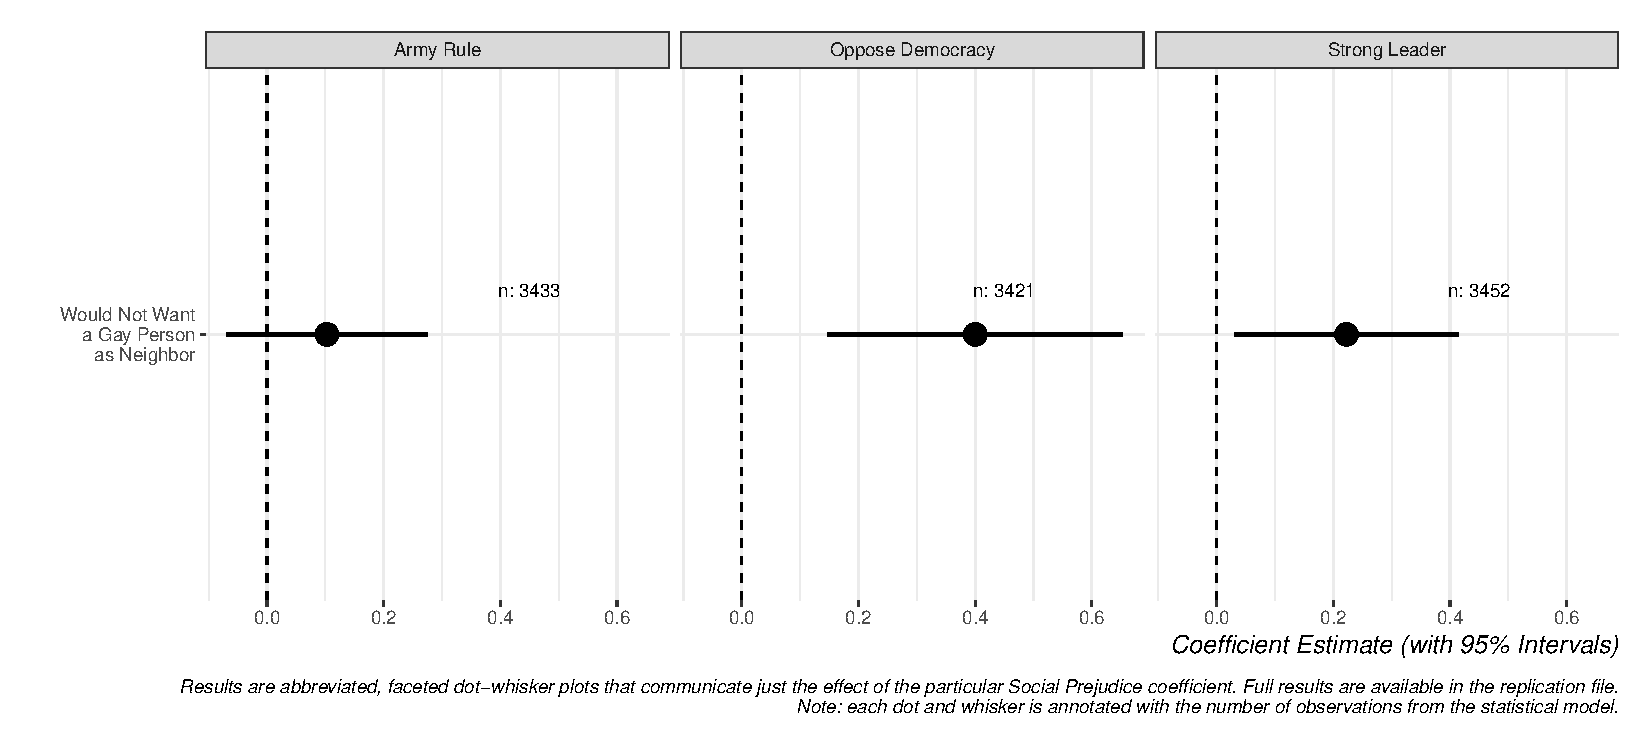
\includegraphics{figs/lgbtseps.pdf}
\caption{\label{fig:lgbtseps}Abbreviated Dot-and-Whisker Plots of the
Effect of Not Wanting a Gay Person for a Neighbor on Anti-Democratic
Orientations}
\end{figure}

\hypertarget{the-effect-of-all-the-neighbor-prompts-on-anti-democratic-orientations}{%
\subsection{The Effect of All the Neighbor Prompts on Anti-Democratic
Orientations}\label{the-effect-of-all-the-neighbor-prompts-on-anti-democratic-orientations}}

We have good theoretical and practical reason to focus our analyses to
white prejudice against racial and ethnic minorities like immigrants,
people of a different race, and people who speak a different language.
However, it might be the case that any of these prompts might coincide
with an anti-democratic orientation and that the analyses we report in
the manuscript, and elsewhere in the appendix, amount to test that just
scrutinizes white supremacists. Toward that end, we loop across all
responses in the individual neighbor prompts and report them as
abbreviated dot-and-whisker plots in Figure
\ref{fig:neighbseps}.\footnote{The prompts for extremists, Jews, and
  militant minorities appear in just one survey wave and thus have no
  temporal heterogeneity to model. The prompts for criminals, those who
  speak a different language, people from a different religion,
  emotionally unstable people, Muslims, and unmarried people appear in
  just two survey waves. We model those analyses with fixed effects for
  survey year. All other prompts appear in all four waves of the WVS
  data and we model those with random effects for the survey year.}

\begin{figure}
\centering
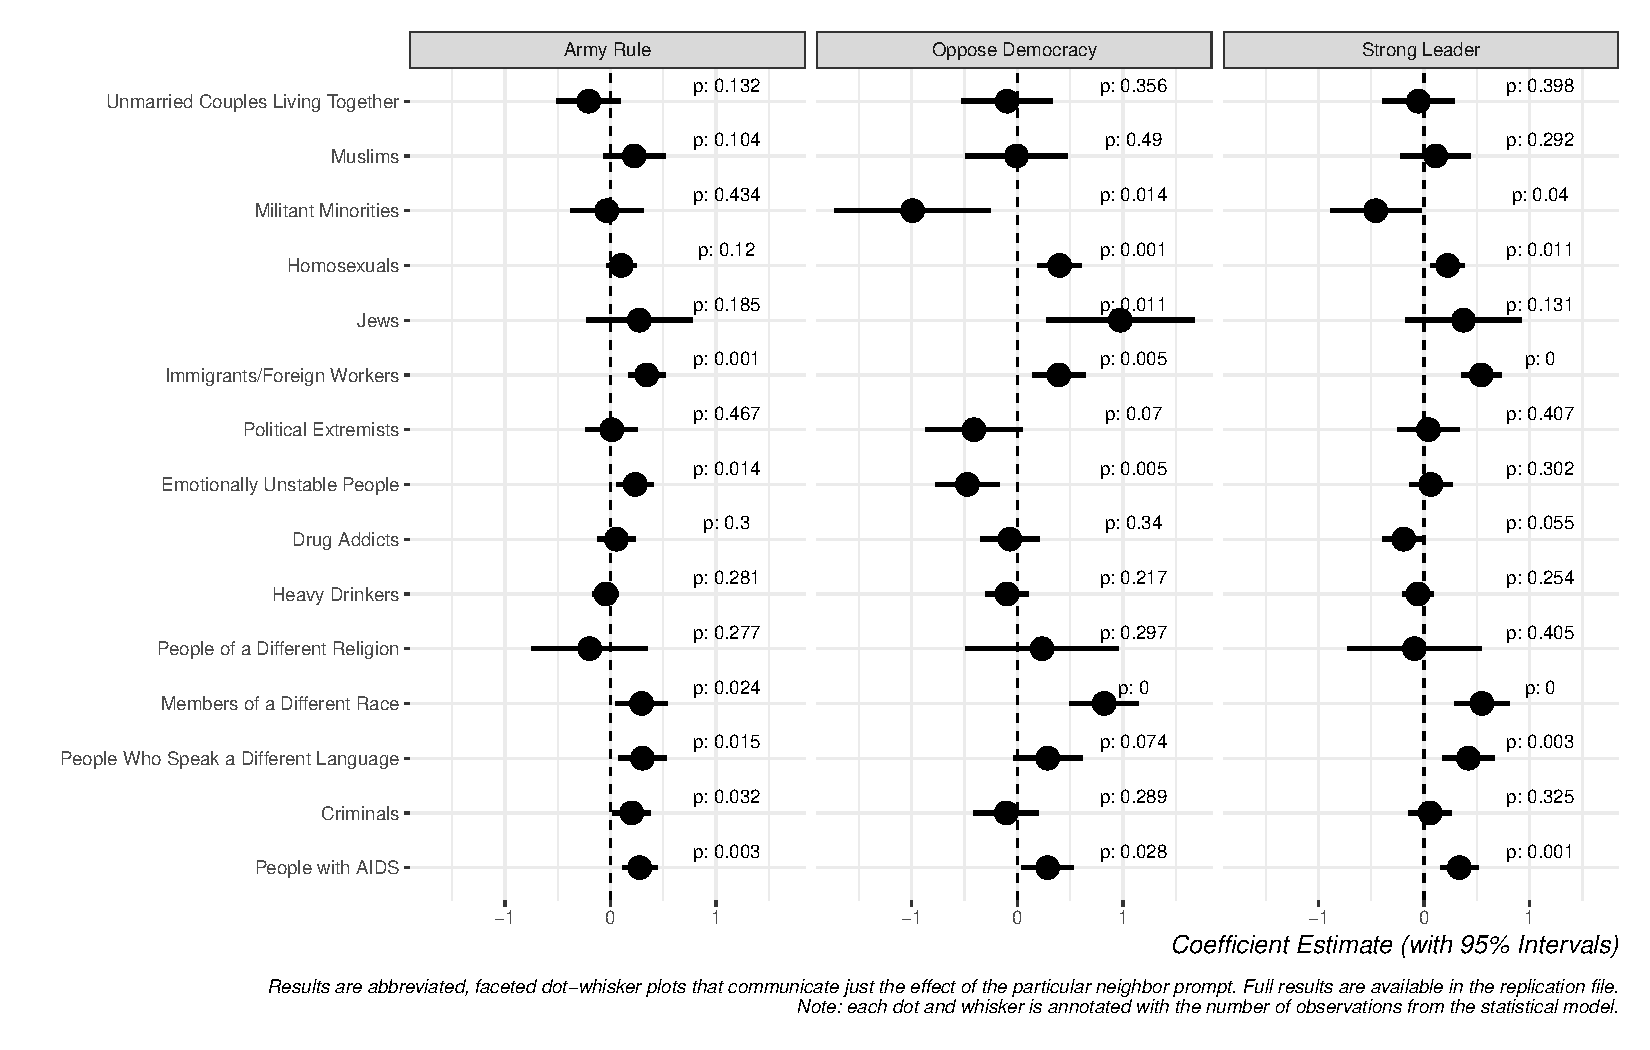
\includegraphics{figs/neighbseps.pdf}
\caption{\label{fig:neighbseps}Abbreviated Dot-and-Whisker Plots of the
Effect of All the Neighbor Prompts on Anti-Democratic Orientations}
\end{figure}

The results lend some confidence to our argument that there is good
theoretical and practical reason to focus on white prejudice against
racial and ethnic minorities. Simply listing heavy drinkers as unwelcome
neighbors, for example, was not enough to induce an anti-democratic
orientation in any survey prompt. Listing emotionally unstable people
also did not have a robust effect across all three models. There would
be no theoretical reason to believe it should have that effect. Indeed,
there are only four of the neighbor prompts that are positive and
statistically significant at least at the .1 level for all three models.
Three of them are the prompts we include in our white social prejudice
variable. The only other one is the responses toward people with AIDS.

\hypertarget{experimenting-with-different-considerations-of-temporal-and-spatial-heterogeneity}{%
\subsection{Experimenting With Different Considerations of Temporal (and
Spatial)
Heterogeneity}\label{experimenting-with-different-considerations-of-temporal-and-spatial-heterogeneity}}

We chose to be flexible with how we address unit heterogeneity in the
data. We modeled the temporal heterogeneity but it is conceivable there
is also spatial heterogeneity in which Americans in the South, for
example, cluster more than Americans in the Northeast. Thus, we follow
\citet{schmidtcatranfairbrother2015remm}, who argue that the best way to
handle spatial and temporal heterogeneity in survey data like the World
Values Survey is to include random effects for the spatial unit, the
year of observation, and the intersection of the spatial unit and the
year. This creates random effects in our analysis for the survey year
(i.e.~1995, 1999, 2006, 2011), the Census region (i.e.~Midwest,
Northeast, South, West), and the Census region-year (e.g.~South-2011,
West-1995, Midwest-2006). We model all random effects with weakly
informative Wishart priors on the covariance matrices
\citep[c.f.][]{chungetal2015wip} given the relatively few number of
categories. We report these analyses in Table \ref{tab:censusyeartab},
showing that the results are almost identical to the inferences we
report in the manuscript's Figure 2.

 
  \providecommand{\huxb}[2]{\arrayrulecolor[RGB]{#1}\global\arrayrulewidth=#2pt}
  \providecommand{\huxvb}[2]{\color[RGB]{#1}\vrule width #2pt}
  \providecommand{\huxtpad}[1]{\rule{0pt}{\baselineskip+#1}}
  \providecommand{\huxbpad}[1]{\rule[-#1]{0pt}{#1}}

\begin{table}[!htbp]
\centering
\begin{threeparttable}
\captionsetup{justification=centering,singlelinecheck=off}
\caption{\label{tab:censusyeartab}The Covariates of Democratic Orientations of White Americans in the World Values Survey [with Spatial-Temporal Random Effects] (1995-2011)}
\begin{tabularx}{0.75\textwidth}{p{0.1875\textwidth} p{0.1875\textwidth} p{0.1875\textwidth} p{0.1875\textwidth}}


\hhline{>{\huxb{0, 0, 0}{0.8}}->{\huxb{0, 0, 0}{0.8}}->{\huxb{0, 0, 0}{0.8}}->{\huxb{0, 0, 0}{0.8}}-}
\arrayrulecolor{black}

\multicolumn{1}{!{\huxvb{0, 0, 0}{0}}c!{\huxvb{0, 0, 0}{0}}}{\huxtpad{4pt}\centering \huxbpad{4pt}} &
\multicolumn{1}{c!{\huxvb{0, 0, 0}{0}}}{\huxtpad{4pt}\centering \textbf{AM13}\huxbpad{4pt}} &
\multicolumn{1}{c!{\huxvb{0, 0, 0}{0}}}{\huxtpad{4pt}\centering \textbf{AM14}\huxbpad{4pt}} &
\multicolumn{1}{c!{\huxvb{0, 0, 0}{0}}}{\huxtpad{4pt}\centering \textbf{AM15}\huxbpad{4pt}} \tabularnewline[-0.5pt]


\hhline{>{\huxb{255, 255, 255}{0.4}}->{\huxb{0, 0, 0}{0.4}}->{\huxb{0, 0, 0}{0.4}}->{\huxb{0, 0, 0}{0.4}}-}
\arrayrulecolor{black}

\multicolumn{1}{!{\huxvb{0, 0, 0}{0}}c!{\huxvb{0, 0, 0}{0}}}{\huxtpad{4pt}\centering \huxbpad{4pt}} &
\multicolumn{1}{c!{\huxvb{0, 0, 0}{0}}}{\huxtpad{4pt}\centering \textit{Strong}\huxbpad{4pt}} &
\multicolumn{1}{c!{\huxvb{0, 0, 0}{0}}}{\huxtpad{4pt}\centering \textit{Army}\huxbpad{4pt}} &
\multicolumn{1}{c!{\huxvb{0, 0, 0}{0}}}{\huxtpad{4pt}\centering \textit{Oppose}\huxbpad{4pt}} \tabularnewline[-0.5pt]


\hhline{}
\arrayrulecolor{black}

\multicolumn{1}{!{\huxvb{0, 0, 0}{0}}c!{\huxvb{0, 0, 0}{0}}}{\huxtpad{4pt}\centering \huxbpad{4pt}} &
\multicolumn{1}{c!{\huxvb{0, 0, 0}{0}}}{\huxtpad{4pt}\centering \textit{Leader}\huxbpad{4pt}} &
\multicolumn{1}{c!{\huxvb{0, 0, 0}{0}}}{\huxtpad{4pt}\centering \textit{Rule}\huxbpad{4pt}} &
\multicolumn{1}{c!{\huxvb{0, 0, 0}{0}}}{\huxtpad{4pt}\centering \textit{Democracy}\huxbpad{4pt}} \tabularnewline[-0.5pt]


\hhline{>{\huxb{0, 0, 0}{0.4}}->{\huxb{0, 0, 0}{0.4}}->{\huxb{0, 0, 0}{0.4}}->{\huxb{0, 0, 0}{0.4}}-}
\arrayrulecolor{black}

\multicolumn{1}{!{\huxvb{0, 0, 0}{0}}c!{\huxvb{0, 0, 0}{0}}}{\huxtpad{4pt}\centering \huxbpad{4pt}} &
\multicolumn{1}{c!{\huxvb{0, 0, 0}{0}}}{\huxtpad{4pt}\centering \huxbpad{4pt}} &
\multicolumn{1}{c!{\huxvb{0, 0, 0}{0}}}{\huxtpad{4pt}\centering \huxbpad{4pt}} &
\multicolumn{1}{c!{\huxvb{0, 0, 0}{0}}}{\huxtpad{4pt}\centering \huxbpad{4pt}} \tabularnewline[-0.5pt]


\hhline{}
\arrayrulecolor{black}

\multicolumn{1}{!{\huxvb{0, 0, 0}{0}}l!{\huxvb{0, 0, 0}{0}}}{\huxtpad{4pt}\raggedright Age\huxbpad{4pt}} &
\multicolumn{1}{c!{\huxvb{0, 0, 0}{0}}}{\huxtpad{4pt}\centering -0.437 ***\huxbpad{4pt}} &
\multicolumn{1}{c!{\huxvb{0, 0, 0}{0}}}{\huxtpad{4pt}\centering -0.451 ***\huxbpad{4pt}} &
\multicolumn{1}{c!{\huxvb{0, 0, 0}{0}}}{\huxtpad{4pt}\centering -0.653 ***\huxbpad{4pt}} \tabularnewline[-0.5pt]


\hhline{}
\arrayrulecolor{black}

\multicolumn{1}{!{\huxvb{0, 0, 0}{0}}l!{\huxvb{0, 0, 0}{0}}}{\huxtpad{4pt}\raggedright \huxbpad{4pt}} &
\multicolumn{1}{c!{\huxvb{0, 0, 0}{0}}}{\huxtpad{4pt}\centering (0.088)\huxbpad{4pt}} &
\multicolumn{1}{c!{\huxvb{0, 0, 0}{0}}}{\huxtpad{4pt}\centering (0.077)\huxbpad{4pt}} &
\multicolumn{1}{c!{\huxvb{0, 0, 0}{0}}}{\huxtpad{4pt}\centering (0.122)\huxbpad{4pt}} \tabularnewline[-0.5pt]


\hhline{}
\arrayrulecolor{black}

\multicolumn{1}{!{\huxvb{0, 0, 0}{0}}l!{\huxvb{0, 0, 0}{0}}}{\huxtpad{4pt}\raggedright Age\verb|^|2\huxbpad{4pt}} &
\multicolumn{1}{c!{\huxvb{0, 0, 0}{0}}}{\huxtpad{4pt}\centering 0.137\huxbpad{4pt}} &
\multicolumn{1}{c!{\huxvb{0, 0, 0}{0}}}{\huxtpad{4pt}\centering 0.046\huxbpad{4pt}} &
\multicolumn{1}{c!{\huxvb{0, 0, 0}{0}}}{\huxtpad{4pt}\centering 0.064\huxbpad{4pt}} \tabularnewline[-0.5pt]


\hhline{}
\arrayrulecolor{black}

\multicolumn{1}{!{\huxvb{0, 0, 0}{0}}l!{\huxvb{0, 0, 0}{0}}}{\huxtpad{4pt}\raggedright \huxbpad{4pt}} &
\multicolumn{1}{c!{\huxvb{0, 0, 0}{0}}}{\huxtpad{4pt}\centering (0.159)\huxbpad{4pt}} &
\multicolumn{1}{c!{\huxvb{0, 0, 0}{0}}}{\huxtpad{4pt}\centering (0.140)\huxbpad{4pt}} &
\multicolumn{1}{c!{\huxvb{0, 0, 0}{0}}}{\huxtpad{4pt}\centering (0.226)\huxbpad{4pt}} \tabularnewline[-0.5pt]


\hhline{}
\arrayrulecolor{black}

\multicolumn{1}{!{\huxvb{0, 0, 0}{0}}l!{\huxvb{0, 0, 0}{0}}}{\huxtpad{4pt}\raggedright Female\huxbpad{4pt}} &
\multicolumn{1}{c!{\huxvb{0, 0, 0}{0}}}{\huxtpad{4pt}\centering 0.049\huxbpad{4pt}} &
\multicolumn{1}{c!{\huxvb{0, 0, 0}{0}}}{\huxtpad{4pt}\centering 0.138\huxbpad{4pt}} &
\multicolumn{1}{c!{\huxvb{0, 0, 0}{0}}}{\huxtpad{4pt}\centering 0.575 ***\huxbpad{4pt}} \tabularnewline[-0.5pt]


\hhline{}
\arrayrulecolor{black}

\multicolumn{1}{!{\huxvb{0, 0, 0}{0}}l!{\huxvb{0, 0, 0}{0}}}{\huxtpad{4pt}\raggedright \huxbpad{4pt}} &
\multicolumn{1}{c!{\huxvb{0, 0, 0}{0}}}{\huxtpad{4pt}\centering (0.084)\huxbpad{4pt}} &
\multicolumn{1}{c!{\huxvb{0, 0, 0}{0}}}{\huxtpad{4pt}\centering (0.072)\huxbpad{4pt}} &
\multicolumn{1}{c!{\huxvb{0, 0, 0}{0}}}{\huxtpad{4pt}\centering (0.120)\huxbpad{4pt}} \tabularnewline[-0.5pt]


\hhline{}
\arrayrulecolor{black}

\multicolumn{1}{!{\huxvb{0, 0, 0}{0}}l!{\huxvb{0, 0, 0}{0}}}{\huxtpad{4pt}\raggedright College Educated\huxbpad{4pt}} &
\multicolumn{1}{c!{\huxvb{0, 0, 0}{0}}}{\huxtpad{4pt}\centering -0.573 ***\huxbpad{4pt}} &
\multicolumn{1}{c!{\huxvb{0, 0, 0}{0}}}{\huxtpad{4pt}\centering -0.162\huxbpad{4pt}} &
\multicolumn{1}{c!{\huxvb{0, 0, 0}{0}}}{\huxtpad{4pt}\centering -1.097 ***\huxbpad{4pt}} \tabularnewline[-0.5pt]


\hhline{}
\arrayrulecolor{black}

\multicolumn{1}{!{\huxvb{0, 0, 0}{0}}l!{\huxvb{0, 0, 0}{0}}}{\huxtpad{4pt}\raggedright \huxbpad{4pt}} &
\multicolumn{1}{c!{\huxvb{0, 0, 0}{0}}}{\huxtpad{4pt}\centering (0.104)\huxbpad{4pt}} &
\multicolumn{1}{c!{\huxvb{0, 0, 0}{0}}}{\huxtpad{4pt}\centering (0.083)\huxbpad{4pt}} &
\multicolumn{1}{c!{\huxvb{0, 0, 0}{0}}}{\huxtpad{4pt}\centering (0.176)\huxbpad{4pt}} \tabularnewline[-0.5pt]


\hhline{}
\arrayrulecolor{black}

\multicolumn{1}{!{\huxvb{0, 0, 0}{0}}l!{\huxvb{0, 0, 0}{0}}}{\huxtpad{4pt}\raggedright Ideology\huxbpad{4pt}} &
\multicolumn{1}{c!{\huxvb{0, 0, 0}{0}}}{\huxtpad{4pt}\centering -0.001\huxbpad{4pt}} &
\multicolumn{1}{c!{\huxvb{0, 0, 0}{0}}}{\huxtpad{4pt}\centering -0.163 *\huxbpad{4pt}} &
\multicolumn{1}{c!{\huxvb{0, 0, 0}{0}}}{\huxtpad{4pt}\centering -0.268\huxbpad{4pt}} \tabularnewline[-0.5pt]


\hhline{}
\arrayrulecolor{black}

\multicolumn{1}{!{\huxvb{0, 0, 0}{0}}l!{\huxvb{0, 0, 0}{0}}}{\huxtpad{4pt}\raggedright \huxbpad{4pt}} &
\multicolumn{1}{c!{\huxvb{0, 0, 0}{0}}}{\huxtpad{4pt}\centering (0.102)\huxbpad{4pt}} &
\multicolumn{1}{c!{\huxvb{0, 0, 0}{0}}}{\huxtpad{4pt}\centering (0.082)\huxbpad{4pt}} &
\multicolumn{1}{c!{\huxvb{0, 0, 0}{0}}}{\huxtpad{4pt}\centering (0.140)\huxbpad{4pt}} \tabularnewline[-0.5pt]


\hhline{}
\arrayrulecolor{black}

\multicolumn{1}{!{\huxvb{0, 0, 0}{0}}l!{\huxvb{0, 0, 0}{0}}}{\huxtpad{4pt}\raggedright Ideology\verb|^|2\huxbpad{4pt}} &
\multicolumn{1}{c!{\huxvb{0, 0, 0}{0}}}{\huxtpad{4pt}\centering -0.520 ***\huxbpad{4pt}} &
\multicolumn{1}{c!{\huxvb{0, 0, 0}{0}}}{\huxtpad{4pt}\centering -0.262 *\huxbpad{4pt}} &
\multicolumn{1}{c!{\huxvb{0, 0, 0}{0}}}{\huxtpad{4pt}\centering -0.122\huxbpad{4pt}} \tabularnewline[-0.5pt]


\hhline{}
\arrayrulecolor{black}

\multicolumn{1}{!{\huxvb{0, 0, 0}{0}}l!{\huxvb{0, 0, 0}{0}}}{\huxtpad{4pt}\raggedright \huxbpad{4pt}} &
\multicolumn{1}{c!{\huxvb{0, 0, 0}{0}}}{\huxtpad{4pt}\centering (0.132)\huxbpad{4pt}} &
\multicolumn{1}{c!{\huxvb{0, 0, 0}{0}}}{\huxtpad{4pt}\centering (0.102)\huxbpad{4pt}} &
\multicolumn{1}{c!{\huxvb{0, 0, 0}{0}}}{\huxtpad{4pt}\centering (0.177)\huxbpad{4pt}} \tabularnewline[-0.5pt]


\hhline{}
\arrayrulecolor{black}

\multicolumn{1}{!{\huxvb{0, 0, 0}{0}}l!{\huxvb{0, 0, 0}{0}}}{\huxtpad{4pt}\raggedright Income Scale\huxbpad{4pt}} &
\multicolumn{1}{c!{\huxvb{0, 0, 0}{0}}}{\huxtpad{4pt}\centering 0.041\huxbpad{4pt}} &
\multicolumn{1}{c!{\huxvb{0, 0, 0}{0}}}{\huxtpad{4pt}\centering -0.013\huxbpad{4pt}} &
\multicolumn{1}{c!{\huxvb{0, 0, 0}{0}}}{\huxtpad{4pt}\centering -0.435 ***\huxbpad{4pt}} \tabularnewline[-0.5pt]


\hhline{}
\arrayrulecolor{black}

\multicolumn{1}{!{\huxvb{0, 0, 0}{0}}l!{\huxvb{0, 0, 0}{0}}}{\huxtpad{4pt}\raggedright \huxbpad{4pt}} &
\multicolumn{1}{c!{\huxvb{0, 0, 0}{0}}}{\huxtpad{4pt}\centering (0.093)\huxbpad{4pt}} &
\multicolumn{1}{c!{\huxvb{0, 0, 0}{0}}}{\huxtpad{4pt}\centering (0.080)\huxbpad{4pt}} &
\multicolumn{1}{c!{\huxvb{0, 0, 0}{0}}}{\huxtpad{4pt}\centering (0.131)\huxbpad{4pt}} \tabularnewline[-0.5pt]


\hhline{}
\arrayrulecolor{black}

\multicolumn{1}{!{\huxvb{0, 0, 0}{0}}l!{\huxvb{0, 0, 0}{0}}}{\huxtpad{4pt}\raggedright Republican\huxbpad{4pt}} &
\multicolumn{1}{c!{\huxvb{0, 0, 0}{0}}}{\huxtpad{4pt}\centering -0.394 **\huxbpad{4pt}} &
\multicolumn{1}{c!{\huxvb{0, 0, 0}{0}}}{\huxtpad{4pt}\centering -0.208\huxbpad{4pt}} &
\multicolumn{1}{c!{\huxvb{0, 0, 0}{0}}}{\huxtpad{4pt}\centering -0.229\huxbpad{4pt}} \tabularnewline[-0.5pt]


\hhline{}
\arrayrulecolor{black}

\multicolumn{1}{!{\huxvb{0, 0, 0}{0}}l!{\huxvb{0, 0, 0}{0}}}{\huxtpad{4pt}\raggedright \huxbpad{4pt}} &
\multicolumn{1}{c!{\huxvb{0, 0, 0}{0}}}{\huxtpad{4pt}\centering (0.131)\huxbpad{4pt}} &
\multicolumn{1}{c!{\huxvb{0, 0, 0}{0}}}{\huxtpad{4pt}\centering (0.116)\huxbpad{4pt}} &
\multicolumn{1}{c!{\huxvb{0, 0, 0}{0}}}{\huxtpad{4pt}\centering (0.162)\huxbpad{4pt}} \tabularnewline[-0.5pt]


\hhline{}
\arrayrulecolor{black}

\multicolumn{1}{!{\huxvb{0, 0, 0}{0}}l!{\huxvb{0, 0, 0}{0}}}{\huxtpad{4pt}\raggedright Democrat\huxbpad{4pt}} &
\multicolumn{1}{c!{\huxvb{0, 0, 0}{0}}}{\huxtpad{4pt}\centering -0.074\huxbpad{4pt}} &
\multicolumn{1}{c!{\huxvb{0, 0, 0}{0}}}{\huxtpad{4pt}\centering -0.071\huxbpad{4pt}} &
\multicolumn{1}{c!{\huxvb{0, 0, 0}{0}}}{\huxtpad{4pt}\centering -1.621 ***\huxbpad{4pt}} \tabularnewline[-0.5pt]


\hhline{}
\arrayrulecolor{black}

\multicolumn{1}{!{\huxvb{0, 0, 0}{0}}l!{\huxvb{0, 0, 0}{0}}}{\huxtpad{4pt}\raggedright \huxbpad{4pt}} &
\multicolumn{1}{c!{\huxvb{0, 0, 0}{0}}}{\huxtpad{4pt}\centering (0.125)\huxbpad{4pt}} &
\multicolumn{1}{c!{\huxvb{0, 0, 0}{0}}}{\huxtpad{4pt}\centering (0.111)\huxbpad{4pt}} &
\multicolumn{1}{c!{\huxvb{0, 0, 0}{0}}}{\huxtpad{4pt}\centering (0.191)\huxbpad{4pt}} \tabularnewline[-0.5pt]


\hhline{}
\arrayrulecolor{black}

\multicolumn{1}{!{\huxvb{0, 0, 0}{0}}l!{\huxvb{0, 0, 0}{0}}}{\huxtpad{4pt}\raggedright Unemployed\huxbpad{4pt}} &
\multicolumn{1}{c!{\huxvb{0, 0, 0}{0}}}{\huxtpad{4pt}\centering 0.516 **\huxbpad{4pt}} &
\multicolumn{1}{c!{\huxvb{0, 0, 0}{0}}}{\huxtpad{4pt}\centering 0.069\huxbpad{4pt}} &
\multicolumn{1}{c!{\huxvb{0, 0, 0}{0}}}{\huxtpad{4pt}\centering 0.686 **\huxbpad{4pt}} \tabularnewline[-0.5pt]


\hhline{}
\arrayrulecolor{black}

\multicolumn{1}{!{\huxvb{0, 0, 0}{0}}l!{\huxvb{0, 0, 0}{0}}}{\huxtpad{4pt}\raggedright \huxbpad{4pt}} &
\multicolumn{1}{c!{\huxvb{0, 0, 0}{0}}}{\huxtpad{4pt}\centering (0.189)\huxbpad{4pt}} &
\multicolumn{1}{c!{\huxvb{0, 0, 0}{0}}}{\huxtpad{4pt}\centering (0.176)\huxbpad{4pt}} &
\multicolumn{1}{c!{\huxvb{0, 0, 0}{0}}}{\huxtpad{4pt}\centering (0.242)\huxbpad{4pt}} \tabularnewline[-0.5pt]


\hhline{}
\arrayrulecolor{black}

\multicolumn{1}{!{\huxvb{0, 0, 0}{0}}l!{\huxvb{0, 0, 0}{0}}}{\huxtpad{4pt}\raggedright Emancipative Values\huxbpad{4pt}} &
\multicolumn{1}{c!{\huxvb{0, 0, 0}{0}}}{\huxtpad{4pt}\centering -0.621 ***\huxbpad{4pt}} &
\multicolumn{1}{c!{\huxvb{0, 0, 0}{0}}}{\huxtpad{4pt}\centering 0.039\huxbpad{4pt}} &
\multicolumn{1}{c!{\huxvb{0, 0, 0}{0}}}{\huxtpad{4pt}\centering -0.674 ***\huxbpad{4pt}} \tabularnewline[-0.5pt]


\hhline{}
\arrayrulecolor{black}

\multicolumn{1}{!{\huxvb{0, 0, 0}{0}}l!{\huxvb{0, 0, 0}{0}}}{\huxtpad{4pt}\raggedright \huxbpad{4pt}} &
\multicolumn{1}{c!{\huxvb{0, 0, 0}{0}}}{\huxtpad{4pt}\centering (0.096)\huxbpad{4pt}} &
\multicolumn{1}{c!{\huxvb{0, 0, 0}{0}}}{\huxtpad{4pt}\centering (0.081)\huxbpad{4pt}} &
\multicolumn{1}{c!{\huxvb{0, 0, 0}{0}}}{\huxtpad{4pt}\centering (0.138)\huxbpad{4pt}} \tabularnewline[-0.5pt]


\hhline{}
\arrayrulecolor{black}

\multicolumn{1}{!{\huxvb{0, 0, 0}{0}}l!{\huxvb{0, 0, 0}{0}}}{\huxtpad{4pt}\raggedright White Social Prejudice\huxbpad{4pt}} &
\multicolumn{1}{c!{\huxvb{0, 0, 0}{0}}}{\huxtpad{4pt}\centering 0.531 ***\huxbpad{4pt}} &
\multicolumn{1}{c!{\huxvb{0, 0, 0}{0}}}{\huxtpad{4pt}\centering 0.367 ***\huxbpad{4pt}} &
\multicolumn{1}{c!{\huxvb{0, 0, 0}{0}}}{\huxtpad{4pt}\centering 0.502 ***\huxbpad{4pt}} \tabularnewline[-0.5pt]


\hhline{}
\arrayrulecolor{black}

\multicolumn{1}{!{\huxvb{0, 0, 0}{0}}l!{\huxvb{0, 0, 0}{0}}}{\huxtpad{4pt}\raggedright \huxbpad{4pt}} &
\multicolumn{1}{c!{\huxvb{0, 0, 0}{0}}}{\huxtpad{4pt}\centering (0.102)\huxbpad{4pt}} &
\multicolumn{1}{c!{\huxvb{0, 0, 0}{0}}}{\huxtpad{4pt}\centering (0.094)\huxbpad{4pt}} &
\multicolumn{1}{c!{\huxvb{0, 0, 0}{0}}}{\huxtpad{4pt}\centering (0.138)\huxbpad{4pt}} \tabularnewline[-0.5pt]


\hhline{}
\arrayrulecolor{black}

\multicolumn{1}{!{\huxvb{0, 0, 0}{0}}l!{\huxvb{0, 0, 0}{0}}}{\huxtpad{4pt}\raggedright \huxbpad{4pt}} &
\multicolumn{1}{c!{\huxvb{0, 0, 0}{0}}}{\huxtpad{4pt}\centering \huxbpad{4pt}} &
\multicolumn{1}{c!{\huxvb{0, 0, 0}{0}}}{\huxtpad{4pt}\centering \huxbpad{4pt}} &
\multicolumn{1}{c!{\huxvb{0, 0, 0}{0}}}{\huxtpad{4pt}\centering \huxbpad{4pt}} \tabularnewline[-0.5pt]


\hhline{}
\arrayrulecolor{black}

\multicolumn{1}{!{\huxvb{0, 0, 0}{0}}l!{\huxvb{0, 0, 0}{0}}}{\huxtpad{4pt}\raggedright \textit{Random Effect}\huxbpad{4pt}} &
\multicolumn{1}{c!{\huxvb{0, 0, 0}{0}}}{\huxtpad{4pt}\centering \huxbpad{4pt}} &
\multicolumn{1}{c!{\huxvb{0, 0, 0}{0}}}{\huxtpad{4pt}\centering \huxbpad{4pt}} &
\multicolumn{1}{c!{\huxvb{0, 0, 0}{0}}}{\huxtpad{4pt}\centering \huxbpad{4pt}} \tabularnewline[-0.5pt]


\hhline{}
\arrayrulecolor{black}

\multicolumn{1}{!{\huxvb{0, 0, 0}{0}}l!{\huxvb{0, 0, 0}{0}}}{\huxtpad{4pt}\raggedright sd(Year)\huxbpad{4pt}} &
\multicolumn{1}{c!{\huxvb{0, 0, 0}{0}}}{\huxtpad{4pt}\centering 0.188\huxbpad{4pt}} &
\multicolumn{1}{c!{\huxvb{0, 0, 0}{0}}}{\huxtpad{4pt}\centering 0.223\huxbpad{4pt}} &
\multicolumn{1}{c!{\huxvb{0, 0, 0}{0}}}{\huxtpad{4pt}\centering 0.313\huxbpad{4pt}} \tabularnewline[-0.5pt]


\hhline{}
\arrayrulecolor{black}

\multicolumn{1}{!{\huxvb{0, 0, 0}{0}}l!{\huxvb{0, 0, 0}{0}}}{\huxtpad{4pt}\raggedright sd(Census Region)\huxbpad{4pt}} &
\multicolumn{1}{c!{\huxvb{0, 0, 0}{0}}}{\huxtpad{4pt}\centering 0.130\huxbpad{4pt}} &
\multicolumn{1}{c!{\huxvb{0, 0, 0}{0}}}{\huxtpad{4pt}\centering 0.090\huxbpad{4pt}} &
\multicolumn{1}{c!{\huxvb{0, 0, 0}{0}}}{\huxtpad{4pt}\centering 0.399\huxbpad{4pt}} \tabularnewline[-0.5pt]


\hhline{}
\arrayrulecolor{black}

\multicolumn{1}{!{\huxvb{0, 0, 0}{0}}l!{\huxvb{0, 0, 0}{0}}}{\huxtpad{4pt}\raggedright sd(Census Region:Year)\huxbpad{4pt}} &
\multicolumn{1}{c!{\huxvb{0, 0, 0}{0}}}{\huxtpad{4pt}\centering 0.195\huxbpad{4pt}} &
\multicolumn{1}{c!{\huxvb{0, 0, 0}{0}}}{\huxtpad{4pt}\centering 0.079\huxbpad{4pt}} &
\multicolumn{1}{c!{\huxvb{0, 0, 0}{0}}}{\huxtpad{4pt}\centering 0.265\huxbpad{4pt}} \tabularnewline[-0.5pt]


\hhline{}
\arrayrulecolor{black}

\multicolumn{1}{!{\huxvb{0, 0, 0}{0}}l!{\huxvb{0, 0, 0}{0}}}{\huxtpad{4pt}\raggedright \huxbpad{4pt}} &
\multicolumn{1}{c!{\huxvb{0, 0, 0}{0}}}{\huxtpad{4pt}\centering \huxbpad{4pt}} &
\multicolumn{1}{c!{\huxvb{0, 0, 0}{0}}}{\huxtpad{4pt}\centering \huxbpad{4pt}} &
\multicolumn{1}{c!{\huxvb{0, 0, 0}{0}}}{\huxtpad{4pt}\centering \huxbpad{4pt}} \tabularnewline[-0.5pt]


\hhline{}
\arrayrulecolor{black}

\multicolumn{1}{!{\huxvb{0, 0, 0}{0}}l!{\huxvb{0, 0, 0}{0}}}{\huxtpad{4pt}\raggedright N\huxbpad{4pt}} &
\multicolumn{1}{c!{\huxvb{0, 0, 0}{0}}}{\huxtpad{4pt}\centering 3432\huxbpad{4pt}} &
\multicolumn{1}{c!{\huxvb{0, 0, 0}{0}}}{\huxtpad{4pt}\centering 3413\huxbpad{4pt}} &
\multicolumn{1}{c!{\huxvb{0, 0, 0}{0}}}{\huxtpad{4pt}\centering 3401\huxbpad{4pt}} \tabularnewline[-0.5pt]


\hhline{>{\huxb{0, 0, 0}{0.8}}->{\huxb{0, 0, 0}{0.8}}->{\huxb{0, 0, 0}{0.8}}->{\huxb{0, 0, 0}{0.8}}-}
\arrayrulecolor{black}

\multicolumn{4}{!{\huxvb{0, 0, 0}{0}}p{0.75\textwidth+6\tabcolsep}!{\huxvb{0, 0, 0}{0}}}{\parbox[b]{0.75\textwidth+6\tabcolsep-4pt-4pt}{\huxtpad{4pt}\raggedright  *** p $<$ 0.001;  ** p $<$ 0.01;  * p $<$ 0.05.\huxbpad{4pt}}} \tabularnewline[-0.5pt]


\hhline{}
\arrayrulecolor{black}
\end{tabularx}\end{threeparttable}


\end{table}
 

Finally, we ran multiple versions of the same model to note that
different techniques for modeling temporal and/or spatial heterogeneity
have no effect on the inferences we report in the analyses. Figure
\ref{fig:fuckitwelldoitlive} is an abbreviated dot-and-whisker plot that
includes the estimates of white social prejudice for estimations in
which we model temporal and/or spatial heterogeneity with 1) just year
random effects (i.e.~the results we report in the manuscript), 2)
region, region-year, and year random effects (i.e.~abbreviated from
Table \ref{tab:censusyeartab}), 3) region and year fixed effects, and 4)
fixed effects for just the year.\footnote{The baselines in the fixed
  effects models are for 1995 (survey year) and the Midwest (Census
  region).} We also re-run the models subsetting the data to each year
(i.e.~individual models for 1995, 1999, 2006, and 2011).

Figure \ref{fig:fuckitwelldoitlive} shows all these effects in the fixed
effects and random effects models are almost identical. The differences
between these estimates are, at most, in the hundredths of a decimal
point of the coefficient and associated \emph{z} statistic. The results
for the individual models that subset the analyses to the individual
survey year are worth highlighting. We want the reader to notice we that
we observe significant effects in all but two estimations. These were
the opppose-democracy model in 1995 and the army-rule model in 1999,
which Figure \ref{fig:barraceyear} suggests were going to be low-power
analyses. Ten of the other 12 estimations yield significant results.

We think this is an important finding from our paper. Our main analyses
leverage all four waves together, offering random effects for the survey
years, to show a general relationship between white social prejudice and
opposition to democracy. This is a current and salient policy discussion
in the age of Trump and there is no shortage of analyses in major
newspapers and academic blogs about how Trump's rhetoric erodes
democratic norms and compromises democratic longevity in the United
States. Our major survey data sets are starting to track these
developments as well. However, we find these trends emerging as early as
1995, a full 20 years before then-candidate Trump first descended his
gilded escalator to begin his presidential campaign with a statement
that Mexicans were rapists and thugs. Our findings at least uncover the
framework that allowed for Trump's rise to power.

\begin{figure}
\centering
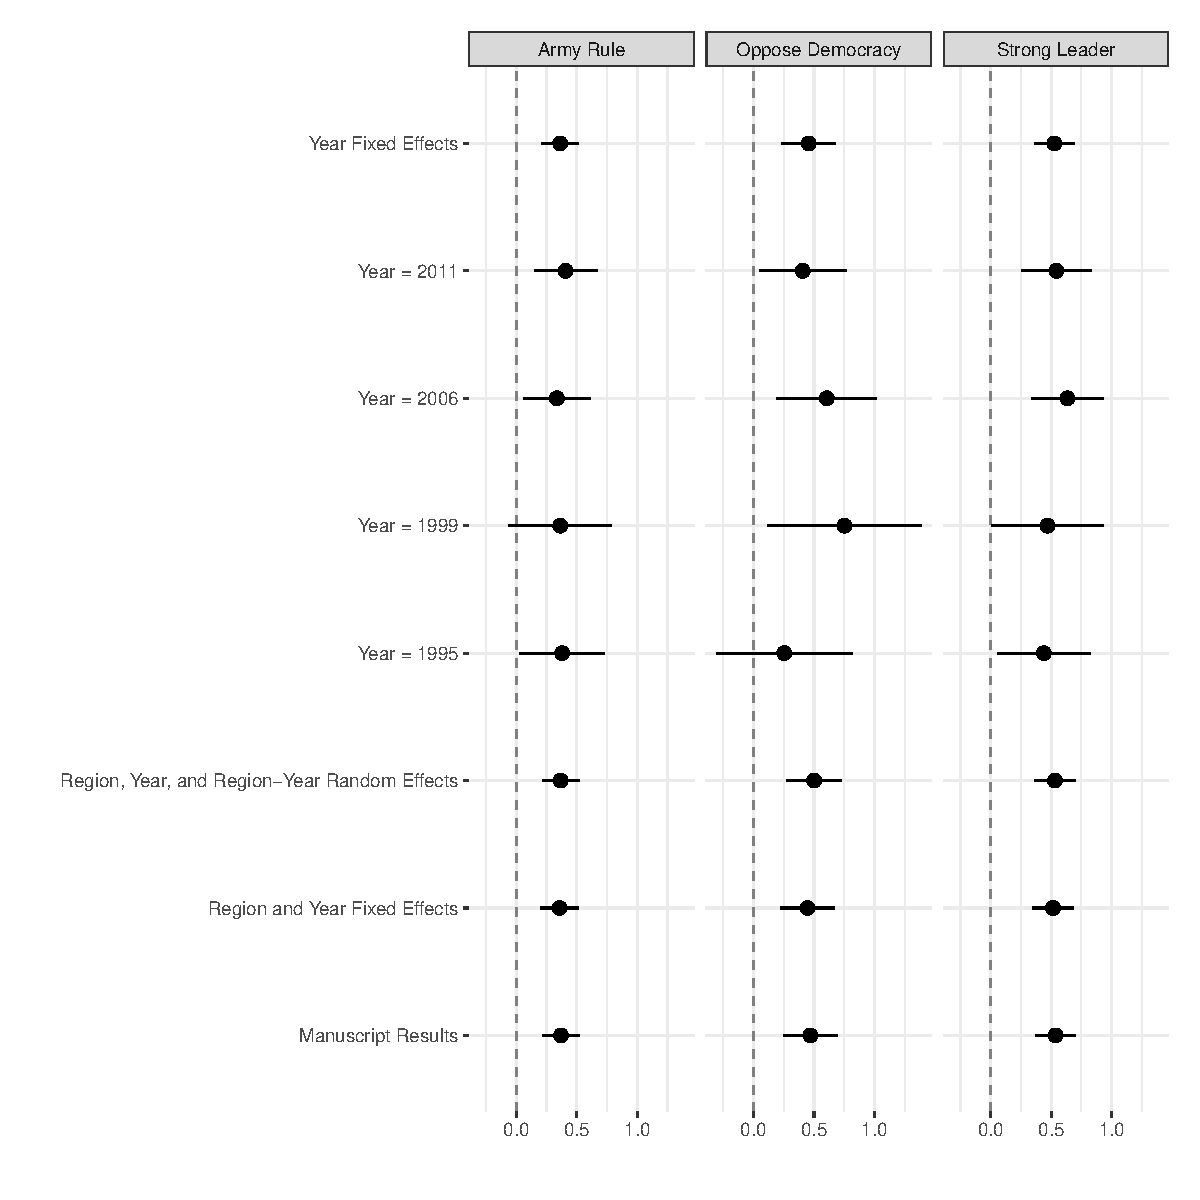
\includegraphics{figs/fuckitwelldoitlive.pdf}
\caption{\label{fig:fuckitwelldoitlive}Dot-and-Whisker Plots of the
Effect of White Social Prejudice Across Multiple Specifications for
Temporal/Spatial Heterogeneity}
\end{figure}

We choose to present the results we do because we think the mixed
effects modeling framework is flexible for the nature of the data. We
also think the random effect for the survey year is an appropriate focus
because of a concern for how these attitudes might be increasing over
time in the U.S. Ultimately, different specifications of spatial and
temporal heterogeneity have no effect on the inferences we report in the
manuscript.

\hypertarget{estimating-the-main-models-as-ordinal-logistic-regressions}{%
\subsection{Estimating the Main Models as Ordinal Logistic
Regressions}\label{estimating-the-main-models-as-ordinal-logistic-regressions}}

We next consider whether our decision to condense the ordinal nature of
the survey items to binary indicators had any effect on our inferences
for the hypothesis of interest. In theory, condensing an ordinal item to
a categorical/``binary'' variable should have no biasing effect on the
regression parameters. It instead introduces noise into the parameters
by condensing information on an ordinal scale to a binary ``there'' or
``not there'' distinction \citep{berryfeldman1985mrp}. Our decision to
present the main analyses as logistic regressions rather than ordinal
logistic regressions comes from a practical concern. We find the
logistic regression to be more intuitive to readers and logistic
regressions spare the reader from having to bother with the ancillary
regression parameters (e.g.~the thresholds) that come with the ordinal
regression framework. However, we conduct a robustness test to see if
this decision for our convenience had any effect on the main independent
variable of interest.

\begin{table}
\begin{center}
\begin{tabular}{l c c c }
\hline
 & \textbf{OM1} & \textbf{OM2} & \textbf{OM3} \\
\hline
Age                         & $-0.513^{***}$ & $-0.475^{***}$ & $-0.563^{***}$ \\
                            & $(0.070)$      & $(0.068)$      & $(0.074)$      \\
Age-squared                 & $0.155$        & $0.162$        & $0.199$        \\
                            & $(0.125)$      & $(0.123)$      & $(0.132)$      \\
Female                      & $0.163^{*}$    & $0.144^{*}$    & $0.298^{***}$  \\
                            & $(0.066)$      & $(0.064)$      & $(0.069)$      \\
College Educated            & $-0.398^{***}$ & $-0.128$       & $-0.450^{***}$ \\
                            & $(0.076)$      & $(0.073)$      & $(0.080)$      \\
Ideology                    & $-0.115$       & $-0.184^{*}$   & $-0.204^{*}$   \\
                            & $(0.077)$      & $(0.073)$      & $(0.081)$      \\
Ideology-squared            & $-0.560^{***}$ & $-0.342^{***}$ & $-0.373^{***}$ \\
                            & $(0.098)$      & $(0.091)$      & $(0.102)$      \\
Income Scale                & $0.043$        & $0.008$        & $-0.349^{***}$ \\
                            & $(0.072)$      & $(0.071)$      & $(0.076)$      \\
Republican                  & $-0.321^{**}$  & $-0.198$       & $-0.343^{**}$  \\
                            & $(0.105)$      & $(0.103)$      & $(0.109)$      \\
Democrat                    & $-0.104$       & $-0.071$       & $-0.883^{***}$ \\
                            & $(0.101)$      & $(0.099)$      & $(0.106)$      \\
Unemployed                  & $0.331^{*}$    & $-0.016$       & $0.320$        \\
                            & $(0.163)$      & $(0.161)$      & $(0.172)$      \\
Emancipative Values         & $-0.665^{***}$ & $-0.043$       & $-0.513^{***}$ \\
                            & $(0.075)$      & $(0.072)$      & $(0.078)$      \\
White Social Prejudice      & $0.429^{***}$  & $0.340^{***}$  & $0.282^{**}$   \\
                            & $(0.086)$      & $(0.084)$      & $(0.090)$      \\
1|2                         & $-0.494^{**}$  & $-1.226^{***}$ & $-0.473^{***}$ \\
                            & $(0.153)$      & $(0.151)$      & $(0.125)$      \\
2|3                         & $0.937^{***}$  & $0.266$        & $1.695^{***}$  \\
                            & $(0.154)$      & $(0.149)$      & $(0.130)$      \\
3|4                         & $2.941^{***}$  & $2.470^{***}$  & $3.045^{***}$  \\
                            & $(0.170)$      & $(0.159)$      & $(0.152)$      \\
\hline
Log Likelihood              & -3899.156      & -4301.916      & -3294.508      \\
AIC                         & 7830.311       & 8635.831       & 6621.015       \\
BIC                         & 7928.659       & 8734.090       & 6719.218       \\
Num. obs.                   & 3452           & 3433           & 3421           \\
Groups (year)               & 4              & 4              & 4              \\
Variance: year: (Intercept) & 0.051          & 0.049          & 0.017          \\
\hline
\multicolumn{4}{l}{\scriptsize{$^{***}p<0.001$, $^{**}p<0.01$, $^*p<0.05$}}
\end{tabular}
\caption{Ordinal Mixed Effects Models of Democratic Orientations of White Americans}
\label{tab:ordinaltab}
\end{center}
\end{table}

Table \ref{tab:ordinaltab} shows the effect of white social prejudice to
be effectively the same when we model the ordinal nature of the survey
responses in lieu of condensing them to binary variables. The effect of
a white American not wanting a neighbor who was an immigrant, of a
different race, or spoke a different language on democratic orientations
is statistically significant across all three estimations. Here, white
social prejudice increases the value a white American puts on having a
strong leader unencumbered by legislative or electoral oversight,
increases the value a white American places on having the U.S. army rule
the government, and \emph{decreases} the value a white American puts on
having a democratic political system in the United States. The
inferences are identical to what we report in the manuscript and
elsewhere in this appendix.

\hypertarget{alternate-measures-of-support-for-american-democracy}{%
\subsection{Alternate Measures of Support for American
Democracy}\label{alternate-measures-of-support-for-american-democracy}}

We offer a final set of robustness tests for the main dependent
variables we model in the manuscript. First, we are interested in an
alternate measure for the ``having a democratic political system''
question we model. That prompt is a regular staple in the WVS data since
the third wave, asking the respondent to say whether ``having a
democratic political system'' is very good, good, bad, or very bad for
the United States. The fifth and sixth waves feature an another question
that gets at the same concept. This question prompts the reader to
answer ``how important is it for you to live in a country that is
governed democratically?'' The responses range from 1 (not at all
important) to 10 (absolutely important).

We ran two linear models on this item. The first resembles Figure 2 in
the manuscript while the second interacts college education with our
white social prejudice measure. Mixed effects modeling collapses to
clasical regression when there are only two groups (i.e.~survey years)
so we forgo the mixed effects framework and include a fixed effect for
2011 compared to the 2006 survey wave.\footnote{Figure
  \ref{fig:fuckitwelldoitlive} lends support to the idea that different
  estimations of spatial and temporal heterogeneity have little-to-no
  effect on the results we report.} The only difference in
interpretation is we expect the effect to be negative. White social
prejudice should decrease the value that white Americans afford to
living in democracy.

 
  \providecommand{\huxb}[2]{\arrayrulecolor[RGB]{#1}\global\arrayrulewidth=#2pt}
  \providecommand{\huxvb}[2]{\color[RGB]{#1}\vrule width #2pt}
  \providecommand{\huxtpad}[1]{\rule{0pt}{\baselineskip+#1}}
  \providecommand{\huxbpad}[1]{\rule[-#1]{0pt}{#1}}

\begin{table}[!htbp]
\centering
\begin{threeparttable}
\captionsetup{justification=centering,singlelinecheck=off}
\caption{\label{tab:demimptab}The Covariates of the Importance of Living in a Democracy for White Americans in the World Values Survey (2006, 2011)}
\begin{tabularx}{0.75\textwidth}{p{0.25\textwidth} p{0.25\textwidth} p{0.25\textwidth}}


\hhline{>{\huxb{0, 0, 0}{0.8}}->{\huxb{0, 0, 0}{0.8}}->{\huxb{0, 0, 0}{0.8}}-}
\arrayrulecolor{black}

\multicolumn{1}{!{\huxvb{0, 0, 0}{0}}c!{\huxvb{0, 0, 0}{0}}}{\huxtpad{4pt}\centering \huxbpad{4pt}} &
\multicolumn{1}{c!{\huxvb{0, 0, 0}{0}}}{\huxtpad{4pt}\centering AM16\huxbpad{4pt}} &
\multicolumn{1}{c!{\huxvb{0, 0, 0}{0}}}{\huxtpad{4pt}\centering AM17\huxbpad{4pt}} \tabularnewline[-0.5pt]


\hhline{>{\huxb{255, 255, 255}{0.4}}->{\huxb{0, 0, 0}{0.4}}->{\huxb{0, 0, 0}{0.4}}-}
\arrayrulecolor{black}

\multicolumn{1}{!{\huxvb{0, 0, 0}{0}}l!{\huxvb{0, 0, 0}{0}}}{\huxtpad{4pt}\raggedright Age\huxbpad{4pt}} &
\multicolumn{1}{c!{\huxvb{0, 0, 0}{0}}}{\huxtpad{4pt}\centering 0.953 ***\huxbpad{4pt}} &
\multicolumn{1}{c!{\huxvb{0, 0, 0}{0}}}{\huxtpad{4pt}\centering 0.956 ***\huxbpad{4pt}} \tabularnewline[-0.5pt]


\hhline{}
\arrayrulecolor{black}

\multicolumn{1}{!{\huxvb{0, 0, 0}{0}}l!{\huxvb{0, 0, 0}{0}}}{\huxtpad{4pt}\raggedright \huxbpad{4pt}} &
\multicolumn{1}{c!{\huxvb{0, 0, 0}{0}}}{\huxtpad{4pt}\centering (0.086)\huxbpad{4pt}} &
\multicolumn{1}{c!{\huxvb{0, 0, 0}{0}}}{\huxtpad{4pt}\centering (0.086)\huxbpad{4pt}} \tabularnewline[-0.5pt]


\hhline{}
\arrayrulecolor{black}

\multicolumn{1}{!{\huxvb{0, 0, 0}{0}}l!{\huxvb{0, 0, 0}{0}}}{\huxtpad{4pt}\raggedright Age\verb|^|2\huxbpad{4pt}} &
\multicolumn{1}{c!{\huxvb{0, 0, 0}{0}}}{\huxtpad{4pt}\centering -0.272\huxbpad{4pt}} &
\multicolumn{1}{c!{\huxvb{0, 0, 0}{0}}}{\huxtpad{4pt}\centering -0.272\huxbpad{4pt}} \tabularnewline[-0.5pt]


\hhline{}
\arrayrulecolor{black}

\multicolumn{1}{!{\huxvb{0, 0, 0}{0}}l!{\huxvb{0, 0, 0}{0}}}{\huxtpad{4pt}\raggedright \huxbpad{4pt}} &
\multicolumn{1}{c!{\huxvb{0, 0, 0}{0}}}{\huxtpad{4pt}\centering (0.152)\huxbpad{4pt}} &
\multicolumn{1}{c!{\huxvb{0, 0, 0}{0}}}{\huxtpad{4pt}\centering (0.152)\huxbpad{4pt}} \tabularnewline[-0.5pt]


\hhline{}
\arrayrulecolor{black}

\multicolumn{1}{!{\huxvb{0, 0, 0}{0}}l!{\huxvb{0, 0, 0}{0}}}{\huxtpad{4pt}\raggedright Female\huxbpad{4pt}} &
\multicolumn{1}{c!{\huxvb{0, 0, 0}{0}}}{\huxtpad{4pt}\centering -0.050\huxbpad{4pt}} &
\multicolumn{1}{c!{\huxvb{0, 0, 0}{0}}}{\huxtpad{4pt}\centering -0.052\huxbpad{4pt}} \tabularnewline[-0.5pt]


\hhline{}
\arrayrulecolor{black}

\multicolumn{1}{!{\huxvb{0, 0, 0}{0}}l!{\huxvb{0, 0, 0}{0}}}{\huxtpad{4pt}\raggedright \huxbpad{4pt}} &
\multicolumn{1}{c!{\huxvb{0, 0, 0}{0}}}{\huxtpad{4pt}\centering (0.079)\huxbpad{4pt}} &
\multicolumn{1}{c!{\huxvb{0, 0, 0}{0}}}{\huxtpad{4pt}\centering (0.079)\huxbpad{4pt}} \tabularnewline[-0.5pt]


\hhline{}
\arrayrulecolor{black}

\multicolumn{1}{!{\huxvb{0, 0, 0}{0}}l!{\huxvb{0, 0, 0}{0}}}{\huxtpad{4pt}\raggedright College Educated\huxbpad{4pt}} &
\multicolumn{1}{c!{\huxvb{0, 0, 0}{0}}}{\huxtpad{4pt}\centering 0.356 ***\huxbpad{4pt}} &
\multicolumn{1}{c!{\huxvb{0, 0, 0}{0}}}{\huxtpad{4pt}\centering 0.297 **\huxbpad{4pt}} \tabularnewline[-0.5pt]


\hhline{}
\arrayrulecolor{black}

\multicolumn{1}{!{\huxvb{0, 0, 0}{0}}l!{\huxvb{0, 0, 0}{0}}}{\huxtpad{4pt}\raggedright \huxbpad{4pt}} &
\multicolumn{1}{c!{\huxvb{0, 0, 0}{0}}}{\huxtpad{4pt}\centering (0.092)\huxbpad{4pt}} &
\multicolumn{1}{c!{\huxvb{0, 0, 0}{0}}}{\huxtpad{4pt}\centering (0.101)\huxbpad{4pt}} \tabularnewline[-0.5pt]


\hhline{}
\arrayrulecolor{black}

\multicolumn{1}{!{\huxvb{0, 0, 0}{0}}l!{\huxvb{0, 0, 0}{0}}}{\huxtpad{4pt}\raggedright Ideology\huxbpad{4pt}} &
\multicolumn{1}{c!{\huxvb{0, 0, 0}{0}}}{\huxtpad{4pt}\centering 0.322 ***\huxbpad{4pt}} &
\multicolumn{1}{c!{\huxvb{0, 0, 0}{0}}}{\huxtpad{4pt}\centering 0.314 **\huxbpad{4pt}} \tabularnewline[-0.5pt]


\hhline{}
\arrayrulecolor{black}

\multicolumn{1}{!{\huxvb{0, 0, 0}{0}}l!{\huxvb{0, 0, 0}{0}}}{\huxtpad{4pt}\raggedright \huxbpad{4pt}} &
\multicolumn{1}{c!{\huxvb{0, 0, 0}{0}}}{\huxtpad{4pt}\centering (0.097)\huxbpad{4pt}} &
\multicolumn{1}{c!{\huxvb{0, 0, 0}{0}}}{\huxtpad{4pt}\centering (0.097)\huxbpad{4pt}} \tabularnewline[-0.5pt]


\hhline{}
\arrayrulecolor{black}

\multicolumn{1}{!{\huxvb{0, 0, 0}{0}}l!{\huxvb{0, 0, 0}{0}}}{\huxtpad{4pt}\raggedright Ideology\verb|^|2\huxbpad{4pt}} &
\multicolumn{1}{c!{\huxvb{0, 0, 0}{0}}}{\huxtpad{4pt}\centering 0.376 ***\huxbpad{4pt}} &
\multicolumn{1}{c!{\huxvb{0, 0, 0}{0}}}{\huxtpad{4pt}\centering 0.379 ***\huxbpad{4pt}} \tabularnewline[-0.5pt]


\hhline{}
\arrayrulecolor{black}

\multicolumn{1}{!{\huxvb{0, 0, 0}{0}}l!{\huxvb{0, 0, 0}{0}}}{\huxtpad{4pt}\raggedright \huxbpad{4pt}} &
\multicolumn{1}{c!{\huxvb{0, 0, 0}{0}}}{\huxtpad{4pt}\centering (0.113)\huxbpad{4pt}} &
\multicolumn{1}{c!{\huxvb{0, 0, 0}{0}}}{\huxtpad{4pt}\centering (0.112)\huxbpad{4pt}} \tabularnewline[-0.5pt]


\hhline{}
\arrayrulecolor{black}

\multicolumn{1}{!{\huxvb{0, 0, 0}{0}}l!{\huxvb{0, 0, 0}{0}}}{\huxtpad{4pt}\raggedright Income Scale\huxbpad{4pt}} &
\multicolumn{1}{c!{\huxvb{0, 0, 0}{0}}}{\huxtpad{4pt}\centering 0.172\huxbpad{4pt}} &
\multicolumn{1}{c!{\huxvb{0, 0, 0}{0}}}{\huxtpad{4pt}\centering 0.173\huxbpad{4pt}} \tabularnewline[-0.5pt]


\hhline{}
\arrayrulecolor{black}

\multicolumn{1}{!{\huxvb{0, 0, 0}{0}}l!{\huxvb{0, 0, 0}{0}}}{\huxtpad{4pt}\raggedright \huxbpad{4pt}} &
\multicolumn{1}{c!{\huxvb{0, 0, 0}{0}}}{\huxtpad{4pt}\centering (0.102)\huxbpad{4pt}} &
\multicolumn{1}{c!{\huxvb{0, 0, 0}{0}}}{\huxtpad{4pt}\centering (0.102)\huxbpad{4pt}} \tabularnewline[-0.5pt]


\hhline{}
\arrayrulecolor{black}

\multicolumn{1}{!{\huxvb{0, 0, 0}{0}}l!{\huxvb{0, 0, 0}{0}}}{\huxtpad{4pt}\raggedright Republican\huxbpad{4pt}} &
\multicolumn{1}{c!{\huxvb{0, 0, 0}{0}}}{\huxtpad{4pt}\centering 0.612 ***\huxbpad{4pt}} &
\multicolumn{1}{c!{\huxvb{0, 0, 0}{0}}}{\huxtpad{4pt}\centering 0.611 ***\huxbpad{4pt}} \tabularnewline[-0.5pt]


\hhline{}
\arrayrulecolor{black}

\multicolumn{1}{!{\huxvb{0, 0, 0}{0}}l!{\huxvb{0, 0, 0}{0}}}{\huxtpad{4pt}\raggedright \huxbpad{4pt}} &
\multicolumn{1}{c!{\huxvb{0, 0, 0}{0}}}{\huxtpad{4pt}\centering (0.133)\huxbpad{4pt}} &
\multicolumn{1}{c!{\huxvb{0, 0, 0}{0}}}{\huxtpad{4pt}\centering (0.133)\huxbpad{4pt}} \tabularnewline[-0.5pt]


\hhline{}
\arrayrulecolor{black}

\multicolumn{1}{!{\huxvb{0, 0, 0}{0}}l!{\huxvb{0, 0, 0}{0}}}{\huxtpad{4pt}\raggedright Democrat\huxbpad{4pt}} &
\multicolumn{1}{c!{\huxvb{0, 0, 0}{0}}}{\huxtpad{4pt}\centering 0.774 ***\huxbpad{4pt}} &
\multicolumn{1}{c!{\huxvb{0, 0, 0}{0}}}{\huxtpad{4pt}\centering 0.772 ***\huxbpad{4pt}} \tabularnewline[-0.5pt]


\hhline{}
\arrayrulecolor{black}

\multicolumn{1}{!{\huxvb{0, 0, 0}{0}}l!{\huxvb{0, 0, 0}{0}}}{\huxtpad{4pt}\raggedright \huxbpad{4pt}} &
\multicolumn{1}{c!{\huxvb{0, 0, 0}{0}}}{\huxtpad{4pt}\centering (0.129)\huxbpad{4pt}} &
\multicolumn{1}{c!{\huxvb{0, 0, 0}{0}}}{\huxtpad{4pt}\centering (0.129)\huxbpad{4pt}} \tabularnewline[-0.5pt]


\hhline{}
\arrayrulecolor{black}

\multicolumn{1}{!{\huxvb{0, 0, 0}{0}}l!{\huxvb{0, 0, 0}{0}}}{\huxtpad{4pt}\raggedright Unemployed\huxbpad{4pt}} &
\multicolumn{1}{c!{\huxvb{0, 0, 0}{0}}}{\huxtpad{4pt}\centering -0.303\huxbpad{4pt}} &
\multicolumn{1}{c!{\huxvb{0, 0, 0}{0}}}{\huxtpad{4pt}\centering -0.318\huxbpad{4pt}} \tabularnewline[-0.5pt]


\hhline{}
\arrayrulecolor{black}

\multicolumn{1}{!{\huxvb{0, 0, 0}{0}}l!{\huxvb{0, 0, 0}{0}}}{\huxtpad{4pt}\raggedright \huxbpad{4pt}} &
\multicolumn{1}{c!{\huxvb{0, 0, 0}{0}}}{\huxtpad{4pt}\centering (0.224)\huxbpad{4pt}} &
\multicolumn{1}{c!{\huxvb{0, 0, 0}{0}}}{\huxtpad{4pt}\centering (0.225)\huxbpad{4pt}} \tabularnewline[-0.5pt]


\hhline{}
\arrayrulecolor{black}

\multicolumn{1}{!{\huxvb{0, 0, 0}{0}}l!{\huxvb{0, 0, 0}{0}}}{\huxtpad{4pt}\raggedright Emancipative Values\huxbpad{4pt}} &
\multicolumn{1}{c!{\huxvb{0, 0, 0}{0}}}{\huxtpad{4pt}\centering 0.348 ***\huxbpad{4pt}} &
\multicolumn{1}{c!{\huxvb{0, 0, 0}{0}}}{\huxtpad{4pt}\centering 0.351 ***\huxbpad{4pt}} \tabularnewline[-0.5pt]


\hhline{}
\arrayrulecolor{black}

\multicolumn{1}{!{\huxvb{0, 0, 0}{0}}l!{\huxvb{0, 0, 0}{0}}}{\huxtpad{4pt}\raggedright \huxbpad{4pt}} &
\multicolumn{1}{c!{\huxvb{0, 0, 0}{0}}}{\huxtpad{4pt}\centering (0.092)\huxbpad{4pt}} &
\multicolumn{1}{c!{\huxvb{0, 0, 0}{0}}}{\huxtpad{4pt}\centering (0.092)\huxbpad{4pt}} \tabularnewline[-0.5pt]


\hhline{}
\arrayrulecolor{black}

\multicolumn{1}{!{\huxvb{0, 0, 0}{0}}l!{\huxvb{0, 0, 0}{0}}}{\huxtpad{4pt}\raggedright White Social Prejudice\huxbpad{4pt}} &
\multicolumn{1}{c!{\huxvb{0, 0, 0}{0}}}{\huxtpad{4pt}\centering -0.339 ***\huxbpad{4pt}} &
\multicolumn{1}{c!{\huxvb{0, 0, 0}{0}}}{\huxtpad{4pt}\centering -0.413 ***\huxbpad{4pt}} \tabularnewline[-0.5pt]


\hhline{}
\arrayrulecolor{black}

\multicolumn{1}{!{\huxvb{0, 0, 0}{0}}l!{\huxvb{0, 0, 0}{0}}}{\huxtpad{4pt}\raggedright \huxbpad{4pt}} &
\multicolumn{1}{c!{\huxvb{0, 0, 0}{0}}}{\huxtpad{4pt}\centering (0.093)\huxbpad{4pt}} &
\multicolumn{1}{c!{\huxvb{0, 0, 0}{0}}}{\huxtpad{4pt}\centering (0.107)\huxbpad{4pt}} \tabularnewline[-0.5pt]


\hhline{}
\arrayrulecolor{black}

\multicolumn{1}{!{\huxvb{0, 0, 0}{0}}l!{\huxvb{0, 0, 0}{0}}}{\huxtpad{4pt}\raggedright White Social Prejudice*College Education\huxbpad{4pt}} &
\multicolumn{1}{c!{\huxvb{0, 0, 0}{0}}}{\huxtpad{4pt}\centering \huxbpad{4pt}} &
\multicolumn{1}{c!{\huxvb{0, 0, 0}{0}}}{\huxtpad{4pt}\centering 0.291\huxbpad{4pt}} \tabularnewline[-0.5pt]


\hhline{}
\arrayrulecolor{black}

\multicolumn{1}{!{\huxvb{0, 0, 0}{0}}l!{\huxvb{0, 0, 0}{0}}}{\huxtpad{4pt}\raggedright \huxbpad{4pt}} &
\multicolumn{1}{c!{\huxvb{0, 0, 0}{0}}}{\huxtpad{4pt}\centering \huxbpad{4pt}} &
\multicolumn{1}{c!{\huxvb{0, 0, 0}{0}}}{\huxtpad{4pt}\centering (0.213)\huxbpad{4pt}} \tabularnewline[-0.5pt]


\hhline{}
\arrayrulecolor{black}

\multicolumn{1}{!{\huxvb{0, 0, 0}{0}}l!{\huxvb{0, 0, 0}{0}}}{\huxtpad{4pt}\raggedright Year = 2011\huxbpad{4pt}} &
\multicolumn{1}{c!{\huxvb{0, 0, 0}{0}}}{\huxtpad{4pt}\centering -0.312 ***\huxbpad{4pt}} &
\multicolumn{1}{c!{\huxvb{0, 0, 0}{0}}}{\huxtpad{4pt}\centering -0.305 ***\huxbpad{4pt}} \tabularnewline[-0.5pt]


\hhline{}
\arrayrulecolor{black}

\multicolumn{1}{!{\huxvb{0, 0, 0}{0}}l!{\huxvb{0, 0, 0}{0}}}{\huxtpad{4pt}\raggedright \huxbpad{4pt}} &
\multicolumn{1}{c!{\huxvb{0, 0, 0}{0}}}{\huxtpad{4pt}\centering (0.083)\huxbpad{4pt}} &
\multicolumn{1}{c!{\huxvb{0, 0, 0}{0}}}{\huxtpad{4pt}\centering (0.083)\huxbpad{4pt}} \tabularnewline[-0.5pt]


\hhline{>{\huxb{255, 255, 255}{0.4}}->{\huxb{0, 0, 0}{0.4}}->{\huxb{0, 0, 0}{0.4}}-}
\arrayrulecolor{black}

\multicolumn{1}{!{\huxvb{0, 0, 0}{0}}l!{\huxvb{0, 0, 0}{0}}}{\huxtpad{4pt}\raggedright N\huxbpad{4pt}} &
\multicolumn{1}{c!{\huxvb{0, 0, 0}{0}}}{\huxtpad{4pt}\centering 1820\huxbpad{4pt}} &
\multicolumn{1}{c!{\huxvb{0, 0, 0}{0}}}{\huxtpad{4pt}\centering 1820\huxbpad{4pt}} \tabularnewline[-0.5pt]


\hhline{}
\arrayrulecolor{black}

\multicolumn{1}{!{\huxvb{0, 0, 0}{0}}l!{\huxvb{0, 0, 0}{0}}}{\huxtpad{4pt}\raggedright R2\huxbpad{4pt}} &
\multicolumn{1}{c!{\huxvb{0, 0, 0}{0}}}{\huxtpad{4pt}\centering 0.132\huxbpad{4pt}} &
\multicolumn{1}{c!{\huxvb{0, 0, 0}{0}}}{\huxtpad{4pt}\centering 0.133\huxbpad{4pt}} \tabularnewline[-0.5pt]


\hhline{}
\arrayrulecolor{black}

\multicolumn{1}{!{\huxvb{0, 0, 0}{0}}l!{\huxvb{0, 0, 0}{0}}}{\huxtpad{4pt}\raggedright logLik\huxbpad{4pt}} &
\multicolumn{1}{c!{\huxvb{0, 0, 0}{0}}}{\huxtpad{4pt}\centering -3497.135\huxbpad{4pt}} &
\multicolumn{1}{c!{\huxvb{0, 0, 0}{0}}}{\huxtpad{4pt}\centering -3496.194\huxbpad{4pt}} \tabularnewline[-0.5pt]


\hhline{}
\arrayrulecolor{black}

\multicolumn{1}{!{\huxvb{0, 0, 0}{0}}l!{\huxvb{0, 0, 0}{0}}}{\huxtpad{4pt}\raggedright AIC\huxbpad{4pt}} &
\multicolumn{1}{c!{\huxvb{0, 0, 0}{0}}}{\huxtpad{4pt}\centering 7024.271\huxbpad{4pt}} &
\multicolumn{1}{c!{\huxvb{0, 0, 0}{0}}}{\huxtpad{4pt}\centering 7024.388\huxbpad{4pt}} \tabularnewline[-0.5pt]


\hhline{>{\huxb{0, 0, 0}{0.8}}->{\huxb{0, 0, 0}{0.8}}->{\huxb{0, 0, 0}{0.8}}-}
\arrayrulecolor{black}

\multicolumn{3}{!{\huxvb{0, 0, 0}{0}}p{0.75\textwidth+4\tabcolsep}!{\huxvb{0, 0, 0}{0}}}{\parbox[b]{0.75\textwidth+4\tabcolsep-4pt-4pt}{\huxtpad{4pt}\raggedright  *** p $<$ 0.001;  ** p $<$ 0.01;  * p $<$ 0.05.\huxbpad{4pt}}} \tabularnewline[-0.5pt]


\hhline{}
\arrayrulecolor{black}
\end{tabularx}\end{threeparttable}


\end{table}
 

Table \ref{tab:demimptab} yields results similar to what we report in
the manuscript and elsewhere in the appendix. The white social prejudice
measure decreases the value that white Americans afford to living in
democracy as much as it makes them open to specific autocratic
alternatives.

Further, we create two indices---one additive and another as a latent
estimate from the factor scores of a graded response model
\citep[c.f.][]{samejima1969ela}---and estimate the analyes as linear
mixed effects models. The results in Table \ref{tab:index} are
substantively identical to what we report in the manuscript. This should
not be surprising since the coefficients for the white social prejudice
variable were robust across all three items that comprise both the
additive index and the latent estimate. The additive index and latent
estimate models communicate similar effects. We also offer the factor
loadings from the graded response model that created the latent
estimate. The information we present communicates that even as the three
items do well to generally communicate anti-democratic orientations in a
cross-national context
\citep[e.g.][]{arielydavidov2011cwr, miller2017etst}, the items do not
necessarily cluster together in the United States.

 
  \providecommand{\huxb}[2]{\arrayrulecolor[RGB]{#1}\global\arrayrulewidth=#2pt}
  \providecommand{\huxvb}[2]{\color[RGB]{#1}\vrule width #2pt}
  \providecommand{\huxtpad}[1]{\rule{0pt}{\baselineskip+#1}}
  \providecommand{\huxbpad}[1]{\rule[-#1]{0pt}{#1}}

\begin{table}[!htbp]
\centering
\begin{threeparttable}
\captionsetup{justification=centering,singlelinecheck=off}
\caption{\label{tab:index}The Covariates of (Indexed) Democratic Orientations of White Americans in the World Values Survey (1995-2011)}
\begin{tabularx}{0.75\textwidth}{p{0.25\textwidth} p{0.25\textwidth} p{0.25\textwidth}}


\hhline{>{\huxb{0, 0, 0}{0.8}}->{\huxb{0, 0, 0}{0.8}}->{\huxb{0, 0, 0}{0.8}}-}
\arrayrulecolor{black}

\multicolumn{1}{!{\huxvb{0, 0, 0}{0}}c!{\huxvb{0, 0, 0}{0}}}{\huxtpad{4pt}\centering \huxbpad{4pt}} &
\multicolumn{1}{c!{\huxvb{0, 0, 0}{0}}}{\huxtpad{4pt}\centering Additive Index\huxbpad{4pt}} &
\multicolumn{1}{c!{\huxvb{0, 0, 0}{0}}}{\huxtpad{4pt}\centering Latent Estimate\huxbpad{4pt}} \tabularnewline[-0.5pt]


\hhline{>{\huxb{255, 255, 255}{0.4}}->{\huxb{0, 0, 0}{0.4}}->{\huxb{0, 0, 0}{0.4}}-}
\arrayrulecolor{black}

\multicolumn{1}{!{\huxvb{0, 0, 0}{0}}l!{\huxvb{0, 0, 0}{0}}}{\huxtpad{4pt}\raggedright Age\huxbpad{4pt}} &
\multicolumn{1}{c!{\huxvb{0, 0, 0}{0}}}{\huxtpad{4pt}\centering -0.652 ***\huxbpad{4pt}} &
\multicolumn{1}{c!{\huxvb{0, 0, 0}{0}}}{\huxtpad{4pt}\centering -0.255 ***\huxbpad{4pt}} \tabularnewline[-0.5pt]


\hhline{}
\arrayrulecolor{black}

\multicolumn{1}{!{\huxvb{0, 0, 0}{0}}l!{\huxvb{0, 0, 0}{0}}}{\huxtpad{4pt}\raggedright \huxbpad{4pt}} &
\multicolumn{1}{c!{\huxvb{0, 0, 0}{0}}}{\huxtpad{4pt}\centering (0.065)\huxbpad{4pt}} &
\multicolumn{1}{c!{\huxvb{0, 0, 0}{0}}}{\huxtpad{4pt}\centering (0.029)\huxbpad{4pt}} \tabularnewline[-0.5pt]


\hhline{}
\arrayrulecolor{black}

\multicolumn{1}{!{\huxvb{0, 0, 0}{0}}l!{\huxvb{0, 0, 0}{0}}}{\huxtpad{4pt}\raggedright Age\verb|^|2\huxbpad{4pt}} &
\multicolumn{1}{c!{\huxvb{0, 0, 0}{0}}}{\huxtpad{4pt}\centering 0.226\huxbpad{4pt}} &
\multicolumn{1}{c!{\huxvb{0, 0, 0}{0}}}{\huxtpad{4pt}\centering 0.087\huxbpad{4pt}} \tabularnewline[-0.5pt]


\hhline{}
\arrayrulecolor{black}

\multicolumn{1}{!{\huxvb{0, 0, 0}{0}}l!{\huxvb{0, 0, 0}{0}}}{\huxtpad{4pt}\raggedright \huxbpad{4pt}} &
\multicolumn{1}{c!{\huxvb{0, 0, 0}{0}}}{\huxtpad{4pt}\centering (0.117)\huxbpad{4pt}} &
\multicolumn{1}{c!{\huxvb{0, 0, 0}{0}}}{\huxtpad{4pt}\centering (0.052)\huxbpad{4pt}} \tabularnewline[-0.5pt]


\hhline{}
\arrayrulecolor{black}

\multicolumn{1}{!{\huxvb{0, 0, 0}{0}}l!{\huxvb{0, 0, 0}{0}}}{\huxtpad{4pt}\raggedright Female\huxbpad{4pt}} &
\multicolumn{1}{c!{\huxvb{0, 0, 0}{0}}}{\huxtpad{4pt}\centering 0.241 ***\huxbpad{4pt}} &
\multicolumn{1}{c!{\huxvb{0, 0, 0}{0}}}{\huxtpad{4pt}\centering 0.072 **\huxbpad{4pt}} \tabularnewline[-0.5pt]


\hhline{}
\arrayrulecolor{black}

\multicolumn{1}{!{\huxvb{0, 0, 0}{0}}l!{\huxvb{0, 0, 0}{0}}}{\huxtpad{4pt}\raggedright \huxbpad{4pt}} &
\multicolumn{1}{c!{\huxvb{0, 0, 0}{0}}}{\huxtpad{4pt}\centering (0.061)\huxbpad{4pt}} &
\multicolumn{1}{c!{\huxvb{0, 0, 0}{0}}}{\huxtpad{4pt}\centering (0.027)\huxbpad{4pt}} \tabularnewline[-0.5pt]


\hhline{}
\arrayrulecolor{black}

\multicolumn{1}{!{\huxvb{0, 0, 0}{0}}l!{\huxvb{0, 0, 0}{0}}}{\huxtpad{4pt}\raggedright College Educated\huxbpad{4pt}} &
\multicolumn{1}{c!{\huxvb{0, 0, 0}{0}}}{\huxtpad{4pt}\centering -0.445 ***\huxbpad{4pt}} &
\multicolumn{1}{c!{\huxvb{0, 0, 0}{0}}}{\huxtpad{4pt}\centering -0.168 ***\huxbpad{4pt}} \tabularnewline[-0.5pt]


\hhline{}
\arrayrulecolor{black}

\multicolumn{1}{!{\huxvb{0, 0, 0}{0}}l!{\huxvb{0, 0, 0}{0}}}{\huxtpad{4pt}\raggedright \huxbpad{4pt}} &
\multicolumn{1}{c!{\huxvb{0, 0, 0}{0}}}{\huxtpad{4pt}\centering (0.070)\huxbpad{4pt}} &
\multicolumn{1}{c!{\huxvb{0, 0, 0}{0}}}{\huxtpad{4pt}\centering (0.031)\huxbpad{4pt}} \tabularnewline[-0.5pt]


\hhline{}
\arrayrulecolor{black}

\multicolumn{1}{!{\huxvb{0, 0, 0}{0}}l!{\huxvb{0, 0, 0}{0}}}{\huxtpad{4pt}\raggedright Ideology\huxbpad{4pt}} &
\multicolumn{1}{c!{\huxvb{0, 0, 0}{0}}}{\huxtpad{4pt}\centering -0.222 **\huxbpad{4pt}} &
\multicolumn{1}{c!{\huxvb{0, 0, 0}{0}}}{\huxtpad{4pt}\centering -0.073 *\huxbpad{4pt}} \tabularnewline[-0.5pt]


\hhline{}
\arrayrulecolor{black}

\multicolumn{1}{!{\huxvb{0, 0, 0}{0}}l!{\huxvb{0, 0, 0}{0}}}{\huxtpad{4pt}\raggedright \huxbpad{4pt}} &
\multicolumn{1}{c!{\huxvb{0, 0, 0}{0}}}{\huxtpad{4pt}\centering (0.069)\huxbpad{4pt}} &
\multicolumn{1}{c!{\huxvb{0, 0, 0}{0}}}{\huxtpad{4pt}\centering (0.031)\huxbpad{4pt}} \tabularnewline[-0.5pt]


\hhline{}
\arrayrulecolor{black}

\multicolumn{1}{!{\huxvb{0, 0, 0}{0}}l!{\huxvb{0, 0, 0}{0}}}{\huxtpad{4pt}\raggedright Ideology\verb|^|2\huxbpad{4pt}} &
\multicolumn{1}{c!{\huxvb{0, 0, 0}{0}}}{\huxtpad{4pt}\centering -0.454 ***\huxbpad{4pt}} &
\multicolumn{1}{c!{\huxvb{0, 0, 0}{0}}}{\huxtpad{4pt}\centering -0.223 ***\huxbpad{4pt}} \tabularnewline[-0.5pt]


\hhline{}
\arrayrulecolor{black}

\multicolumn{1}{!{\huxvb{0, 0, 0}{0}}l!{\huxvb{0, 0, 0}{0}}}{\huxtpad{4pt}\raggedright \huxbpad{4pt}} &
\multicolumn{1}{c!{\huxvb{0, 0, 0}{0}}}{\huxtpad{4pt}\centering (0.085)\huxbpad{4pt}} &
\multicolumn{1}{c!{\huxvb{0, 0, 0}{0}}}{\huxtpad{4pt}\centering (0.038)\huxbpad{4pt}} \tabularnewline[-0.5pt]


\hhline{}
\arrayrulecolor{black}

\multicolumn{1}{!{\huxvb{0, 0, 0}{0}}l!{\huxvb{0, 0, 0}{0}}}{\huxtpad{4pt}\raggedright Income Scale\huxbpad{4pt}} &
\multicolumn{1}{c!{\huxvb{0, 0, 0}{0}}}{\huxtpad{4pt}\centering -0.089\huxbpad{4pt}} &
\multicolumn{1}{c!{\huxvb{0, 0, 0}{0}}}{\huxtpad{4pt}\centering -0.000\huxbpad{4pt}} \tabularnewline[-0.5pt]


\hhline{}
\arrayrulecolor{black}

\multicolumn{1}{!{\huxvb{0, 0, 0}{0}}l!{\huxvb{0, 0, 0}{0}}}{\huxtpad{4pt}\raggedright \huxbpad{4pt}} &
\multicolumn{1}{c!{\huxvb{0, 0, 0}{0}}}{\huxtpad{4pt}\centering (0.067)\huxbpad{4pt}} &
\multicolumn{1}{c!{\huxvb{0, 0, 0}{0}}}{\huxtpad{4pt}\centering (0.030)\huxbpad{4pt}} \tabularnewline[-0.5pt]


\hhline{}
\arrayrulecolor{black}

\multicolumn{1}{!{\huxvb{0, 0, 0}{0}}l!{\huxvb{0, 0, 0}{0}}}{\huxtpad{4pt}\raggedright Republican\huxbpad{4pt}} &
\multicolumn{1}{c!{\huxvb{0, 0, 0}{0}}}{\huxtpad{4pt}\centering -0.387 ***\huxbpad{4pt}} &
\multicolumn{1}{c!{\huxvb{0, 0, 0}{0}}}{\huxtpad{4pt}\centering -0.150 ***\huxbpad{4pt}} \tabularnewline[-0.5pt]


\hhline{}
\arrayrulecolor{black}

\multicolumn{1}{!{\huxvb{0, 0, 0}{0}}l!{\huxvb{0, 0, 0}{0}}}{\huxtpad{4pt}\raggedright \huxbpad{4pt}} &
\multicolumn{1}{c!{\huxvb{0, 0, 0}{0}}}{\huxtpad{4pt}\centering (0.099)\huxbpad{4pt}} &
\multicolumn{1}{c!{\huxvb{0, 0, 0}{0}}}{\huxtpad{4pt}\centering (0.044)\huxbpad{4pt}} \tabularnewline[-0.5pt]


\hhline{}
\arrayrulecolor{black}

\multicolumn{1}{!{\huxvb{0, 0, 0}{0}}l!{\huxvb{0, 0, 0}{0}}}{\huxtpad{4pt}\raggedright Democrat\huxbpad{4pt}} &
\multicolumn{1}{c!{\huxvb{0, 0, 0}{0}}}{\huxtpad{4pt}\centering -0.479 ***\huxbpad{4pt}} &
\multicolumn{1}{c!{\huxvb{0, 0, 0}{0}}}{\huxtpad{4pt}\centering -0.090 *\huxbpad{4pt}} \tabularnewline[-0.5pt]


\hhline{}
\arrayrulecolor{black}

\multicolumn{1}{!{\huxvb{0, 0, 0}{0}}l!{\huxvb{0, 0, 0}{0}}}{\huxtpad{4pt}\raggedright \huxbpad{4pt}} &
\multicolumn{1}{c!{\huxvb{0, 0, 0}{0}}}{\huxtpad{4pt}\centering (0.095)\huxbpad{4pt}} &
\multicolumn{1}{c!{\huxvb{0, 0, 0}{0}}}{\huxtpad{4pt}\centering (0.043)\huxbpad{4pt}} \tabularnewline[-0.5pt]


\hhline{}
\arrayrulecolor{black}

\multicolumn{1}{!{\huxvb{0, 0, 0}{0}}l!{\huxvb{0, 0, 0}{0}}}{\huxtpad{4pt}\raggedright Unemployed\huxbpad{4pt}} &
\multicolumn{1}{c!{\huxvb{0, 0, 0}{0}}}{\huxtpad{4pt}\centering 0.221\huxbpad{4pt}} &
\multicolumn{1}{c!{\huxvb{0, 0, 0}{0}}}{\huxtpad{4pt}\centering 0.079\huxbpad{4pt}} \tabularnewline[-0.5pt]


\hhline{}
\arrayrulecolor{black}

\multicolumn{1}{!{\huxvb{0, 0, 0}{0}}l!{\huxvb{0, 0, 0}{0}}}{\huxtpad{4pt}\raggedright \huxbpad{4pt}} &
\multicolumn{1}{c!{\huxvb{0, 0, 0}{0}}}{\huxtpad{4pt}\centering (0.153)\huxbpad{4pt}} &
\multicolumn{1}{c!{\huxvb{0, 0, 0}{0}}}{\huxtpad{4pt}\centering (0.069)\huxbpad{4pt}} \tabularnewline[-0.5pt]


\hhline{}
\arrayrulecolor{black}

\multicolumn{1}{!{\huxvb{0, 0, 0}{0}}l!{\huxvb{0, 0, 0}{0}}}{\huxtpad{4pt}\raggedright Emancipative Values\huxbpad{4pt}} &
\multicolumn{1}{c!{\huxvb{0, 0, 0}{0}}}{\huxtpad{4pt}\centering -0.502 ***\huxbpad{4pt}} &
\multicolumn{1}{c!{\huxvb{0, 0, 0}{0}}}{\huxtpad{4pt}\centering -0.244 ***\huxbpad{4pt}} \tabularnewline[-0.5pt]


\hhline{}
\arrayrulecolor{black}

\multicolumn{1}{!{\huxvb{0, 0, 0}{0}}l!{\huxvb{0, 0, 0}{0}}}{\huxtpad{4pt}\raggedright \huxbpad{4pt}} &
\multicolumn{1}{c!{\huxvb{0, 0, 0}{0}}}{\huxtpad{4pt}\centering (0.068)\huxbpad{4pt}} &
\multicolumn{1}{c!{\huxvb{0, 0, 0}{0}}}{\huxtpad{4pt}\centering (0.030)\huxbpad{4pt}} \tabularnewline[-0.5pt]


\hhline{}
\arrayrulecolor{black}

\multicolumn{1}{!{\huxvb{0, 0, 0}{0}}l!{\huxvb{0, 0, 0}{0}}}{\huxtpad{4pt}\raggedright White Social Prejudice\huxbpad{4pt}} &
\multicolumn{1}{c!{\huxvb{0, 0, 0}{0}}}{\huxtpad{4pt}\centering 0.494 ***\huxbpad{4pt}} &
\multicolumn{1}{c!{\huxvb{0, 0, 0}{0}}}{\huxtpad{4pt}\centering 0.200 ***\huxbpad{4pt}} \tabularnewline[-0.5pt]


\hhline{}
\arrayrulecolor{black}

\multicolumn{1}{!{\huxvb{0, 0, 0}{0}}l!{\huxvb{0, 0, 0}{0}}}{\huxtpad{4pt}\raggedright \huxbpad{4pt}} &
\multicolumn{1}{c!{\huxvb{0, 0, 0}{0}}}{\huxtpad{4pt}\centering (0.080)\huxbpad{4pt}} &
\multicolumn{1}{c!{\huxvb{0, 0, 0}{0}}}{\huxtpad{4pt}\centering (0.036)\huxbpad{4pt}} \tabularnewline[-0.5pt]


\hhline{>{\huxb{255, 255, 255}{0.4}}->{\huxb{0, 0, 0}{0.4}}->{\huxb{0, 0, 0}{0.4}}-}
\arrayrulecolor{black}

\multicolumn{1}{!{\huxvb{0, 0, 0}{0}}l!{\huxvb{0, 0, 0}{0}}}{\huxtpad{4pt}\raggedright N\huxbpad{4pt}} &
\multicolumn{1}{c!{\huxvb{0, 0, 0}{0}}}{\huxtpad{4pt}\centering 3368\huxbpad{4pt}} &
\multicolumn{1}{c!{\huxvb{0, 0, 0}{0}}}{\huxtpad{4pt}\centering 3368\huxbpad{4pt}} \tabularnewline[-0.5pt]


\hhline{>{\huxb{0, 0, 0}{0.8}}->{\huxb{0, 0, 0}{0.8}}->{\huxb{0, 0, 0}{0.8}}-}
\arrayrulecolor{black}

\multicolumn{3}{!{\huxvb{0, 0, 0}{0}}p{0.75\textwidth+4\tabcolsep}!{\huxvb{0, 0, 0}{0}}}{\parbox[b]{0.75\textwidth+4\tabcolsep-4pt-4pt}{\huxtpad{4pt}\raggedright  *** p $<$ 0.001;  ** p $<$ 0.01;  * p $<$ 0.05.\huxbpad{4pt}}} \tabularnewline[-0.5pt]


\hhline{}
\arrayrulecolor{black}
\end{tabularx}\end{threeparttable}


\end{table}
 

\begin{table}[t]

\caption{\label{tab:indexfscores}The Factor Loadings from the Graded Response Model for the Latent Estimate}
\centering
\begin{tabular}{lc}
\toprule
Variable & Factor Loading\\
\midrule
Oppose Democracy & 0.309\\
Strong Leader & 0.899\\
Army Rule & 0.610\\
\bottomrule
\end{tabular}
\end{table}

Finally, we unpack the implications of \citet{welzel2013fr}. Welzel
created a four-item index of what he terms ``emancipative values'',
which consist of sub-values of ``autonomy'', ``choice'', ``equality'',
and ``voice.'' The voice component of the emancipative values framework
is of particular interest here because it also communicates democratic
orientations similar to the ones we measure through the manuscript and
appendix. After all, the ``voice'' variable is measuring the relative
importance the respondent gives to allowing more people more say in
politics as both an important national priority and a personal political
priority. The question prompt is deliberately worded so that the
``people'' in question are not the respondent, but others different from
the respondent. Per our theory, a white American prejudiced against
ethnic and racial minorities should be less likely to prioritize
allowing more people more say in politics since this should also entail
enfranchising the people against whom the respondent is prejudiced.

Table \ref{tab:lvoi} communicates the results of two models that explain
variation in the voice variable we estimate and include as part of the
emancipative values variable. The first model in Table \ref{tab:lvoi}
excludes the other values that comprise the emancipative values variable
while the second model includes them as additional covariates. We find
robust negative effects for the white social prejudice variable on the
voice variable. A white respondent who would not want an
immigrant/foreign worker, member of a different race, or a person who
speaks a different language as a neighbor scores lower on the voice
variable (i.e.~is less likely to prioritize giving people more of a say
in politics, per the construction of the variable). While we observe
evidence that suggests the voice value as a dependent variable to be
explained comports nicely with the main analyses we present in the
manuscript, the results we provide in Table \ref{tab:emanc}---which
breaks apart the emancipative values variable from our main analyses to
its four individual components---suggest the voice variable does not
have a robust effect on anti-democratic orientations.

 
  \providecommand{\huxb}[2]{\arrayrulecolor[RGB]{#1}\global\arrayrulewidth=#2pt}
  \providecommand{\huxvb}[2]{\color[RGB]{#1}\vrule width #2pt}
  \providecommand{\huxtpad}[1]{\rule{0pt}{\baselineskip+#1}}
  \providecommand{\huxbpad}[1]{\rule[-#1]{0pt}{#1}}

\begin{table}[!htbp]
\centering
\begin{threeparttable}
\captionsetup{justification=centering,singlelinecheck=off}
\caption{\label{tab:lvoi}The Covariates of Voice Values of White Americans in the World Values Survey (1995-2011)}
\begin{tabularx}{0.75\textwidth}{p{0.25\textwidth} p{0.25\textwidth} p{0.25\textwidth}}


\hhline{>{\huxb{0, 0, 0}{0.8}}->{\huxb{0, 0, 0}{0.8}}->{\huxb{0, 0, 0}{0.8}}-}
\arrayrulecolor{black}

\multicolumn{1}{!{\huxvb{0, 0, 0}{0}}c!{\huxvb{0, 0, 0}{0}}}{\huxtpad{4pt}\centering \huxbpad{4pt}} &
\multicolumn{1}{c!{\huxvb{0, 0, 0}{0}}}{\huxtpad{4pt}\centering AM20\huxbpad{4pt}} &
\multicolumn{1}{c!{\huxvb{0, 0, 0}{0}}}{\huxtpad{4pt}\centering AM21\huxbpad{4pt}} \tabularnewline[-0.5pt]


\hhline{>{\huxb{255, 255, 255}{0.4}}->{\huxb{0, 0, 0}{0.4}}->{\huxb{0, 0, 0}{0.4}}-}
\arrayrulecolor{black}

\multicolumn{1}{!{\huxvb{0, 0, 0}{0}}l!{\huxvb{0, 0, 0}{0}}}{\huxtpad{4pt}\raggedright Age\huxbpad{4pt}} &
\multicolumn{1}{c!{\huxvb{0, 0, 0}{0}}}{\huxtpad{4pt}\centering -0.167 ***\huxbpad{4pt}} &
\multicolumn{1}{c!{\huxvb{0, 0, 0}{0}}}{\huxtpad{4pt}\centering -0.150 ***\huxbpad{4pt}} \tabularnewline[-0.5pt]


\hhline{}
\arrayrulecolor{black}

\multicolumn{1}{!{\huxvb{0, 0, 0}{0}}l!{\huxvb{0, 0, 0}{0}}}{\huxtpad{4pt}\raggedright \huxbpad{4pt}} &
\multicolumn{1}{c!{\huxvb{0, 0, 0}{0}}}{\huxtpad{4pt}\centering (0.026)\huxbpad{4pt}} &
\multicolumn{1}{c!{\huxvb{0, 0, 0}{0}}}{\huxtpad{4pt}\centering (0.026)\huxbpad{4pt}} \tabularnewline[-0.5pt]


\hhline{}
\arrayrulecolor{black}

\multicolumn{1}{!{\huxvb{0, 0, 0}{0}}l!{\huxvb{0, 0, 0}{0}}}{\huxtpad{4pt}\raggedright Age\verb|^|2\huxbpad{4pt}} &
\multicolumn{1}{c!{\huxvb{0, 0, 0}{0}}}{\huxtpad{4pt}\centering 0.023\huxbpad{4pt}} &
\multicolumn{1}{c!{\huxvb{0, 0, 0}{0}}}{\huxtpad{4pt}\centering 0.045\huxbpad{4pt}} \tabularnewline[-0.5pt]


\hhline{}
\arrayrulecolor{black}

\multicolumn{1}{!{\huxvb{0, 0, 0}{0}}l!{\huxvb{0, 0, 0}{0}}}{\huxtpad{4pt}\raggedright \huxbpad{4pt}} &
\multicolumn{1}{c!{\huxvb{0, 0, 0}{0}}}{\huxtpad{4pt}\centering (0.046)\huxbpad{4pt}} &
\multicolumn{1}{c!{\huxvb{0, 0, 0}{0}}}{\huxtpad{4pt}\centering (0.047)\huxbpad{4pt}} \tabularnewline[-0.5pt]


\hhline{}
\arrayrulecolor{black}

\multicolumn{1}{!{\huxvb{0, 0, 0}{0}}l!{\huxvb{0, 0, 0}{0}}}{\huxtpad{4pt}\raggedright Female\huxbpad{4pt}} &
\multicolumn{1}{c!{\huxvb{0, 0, 0}{0}}}{\huxtpad{4pt}\centering 0.008\huxbpad{4pt}} &
\multicolumn{1}{c!{\huxvb{0, 0, 0}{0}}}{\huxtpad{4pt}\centering -0.015\huxbpad{4pt}} \tabularnewline[-0.5pt]


\hhline{}
\arrayrulecolor{black}

\multicolumn{1}{!{\huxvb{0, 0, 0}{0}}l!{\huxvb{0, 0, 0}{0}}}{\huxtpad{4pt}\raggedright \huxbpad{4pt}} &
\multicolumn{1}{c!{\huxvb{0, 0, 0}{0}}}{\huxtpad{4pt}\centering (0.024)\huxbpad{4pt}} &
\multicolumn{1}{c!{\huxvb{0, 0, 0}{0}}}{\huxtpad{4pt}\centering (0.025)\huxbpad{4pt}} \tabularnewline[-0.5pt]


\hhline{}
\arrayrulecolor{black}

\multicolumn{1}{!{\huxvb{0, 0, 0}{0}}l!{\huxvb{0, 0, 0}{0}}}{\huxtpad{4pt}\raggedright College Educated\huxbpad{4pt}} &
\multicolumn{1}{c!{\huxvb{0, 0, 0}{0}}}{\huxtpad{4pt}\centering 0.068 *\huxbpad{4pt}} &
\multicolumn{1}{c!{\huxvb{0, 0, 0}{0}}}{\huxtpad{4pt}\centering 0.042\huxbpad{4pt}} \tabularnewline[-0.5pt]


\hhline{}
\arrayrulecolor{black}

\multicolumn{1}{!{\huxvb{0, 0, 0}{0}}l!{\huxvb{0, 0, 0}{0}}}{\huxtpad{4pt}\raggedright \huxbpad{4pt}} &
\multicolumn{1}{c!{\huxvb{0, 0, 0}{0}}}{\huxtpad{4pt}\centering (0.027)\huxbpad{4pt}} &
\multicolumn{1}{c!{\huxvb{0, 0, 0}{0}}}{\huxtpad{4pt}\centering (0.028)\huxbpad{4pt}} \tabularnewline[-0.5pt]


\hhline{}
\arrayrulecolor{black}

\multicolumn{1}{!{\huxvb{0, 0, 0}{0}}l!{\huxvb{0, 0, 0}{0}}}{\huxtpad{4pt}\raggedright Ideology\huxbpad{4pt}} &
\multicolumn{1}{c!{\huxvb{0, 0, 0}{0}}}{\huxtpad{4pt}\centering -0.195 ***\huxbpad{4pt}} &
\multicolumn{1}{c!{\huxvb{0, 0, 0}{0}}}{\huxtpad{4pt}\centering -0.168 ***\huxbpad{4pt}} \tabularnewline[-0.5pt]


\hhline{}
\arrayrulecolor{black}

\multicolumn{1}{!{\huxvb{0, 0, 0}{0}}l!{\huxvb{0, 0, 0}{0}}}{\huxtpad{4pt}\raggedright \huxbpad{4pt}} &
\multicolumn{1}{c!{\huxvb{0, 0, 0}{0}}}{\huxtpad{4pt}\centering (0.027)\huxbpad{4pt}} &
\multicolumn{1}{c!{\huxvb{0, 0, 0}{0}}}{\huxtpad{4pt}\centering (0.027)\huxbpad{4pt}} \tabularnewline[-0.5pt]


\hhline{}
\arrayrulecolor{black}

\multicolumn{1}{!{\huxvb{0, 0, 0}{0}}l!{\huxvb{0, 0, 0}{0}}}{\huxtpad{4pt}\raggedright Ideology\verb|^|2\huxbpad{4pt}} &
\multicolumn{1}{c!{\huxvb{0, 0, 0}{0}}}{\huxtpad{4pt}\centering 0.171 ***\huxbpad{4pt}} &
\multicolumn{1}{c!{\huxvb{0, 0, 0}{0}}}{\huxtpad{4pt}\centering 0.168 ***\huxbpad{4pt}} \tabularnewline[-0.5pt]


\hhline{}
\arrayrulecolor{black}

\multicolumn{1}{!{\huxvb{0, 0, 0}{0}}l!{\huxvb{0, 0, 0}{0}}}{\huxtpad{4pt}\raggedright \huxbpad{4pt}} &
\multicolumn{1}{c!{\huxvb{0, 0, 0}{0}}}{\huxtpad{4pt}\centering (0.034)\huxbpad{4pt}} &
\multicolumn{1}{c!{\huxvb{0, 0, 0}{0}}}{\huxtpad{4pt}\centering (0.034)\huxbpad{4pt}} \tabularnewline[-0.5pt]


\hhline{}
\arrayrulecolor{black}

\multicolumn{1}{!{\huxvb{0, 0, 0}{0}}l!{\huxvb{0, 0, 0}{0}}}{\huxtpad{4pt}\raggedright Income Scale\huxbpad{4pt}} &
\multicolumn{1}{c!{\huxvb{0, 0, 0}{0}}}{\huxtpad{4pt}\centering -0.033\huxbpad{4pt}} &
\multicolumn{1}{c!{\huxvb{0, 0, 0}{0}}}{\huxtpad{4pt}\centering -0.040\huxbpad{4pt}} \tabularnewline[-0.5pt]


\hhline{}
\arrayrulecolor{black}

\multicolumn{1}{!{\huxvb{0, 0, 0}{0}}l!{\huxvb{0, 0, 0}{0}}}{\huxtpad{4pt}\raggedright \huxbpad{4pt}} &
\multicolumn{1}{c!{\huxvb{0, 0, 0}{0}}}{\huxtpad{4pt}\centering (0.026)\huxbpad{4pt}} &
\multicolumn{1}{c!{\huxvb{0, 0, 0}{0}}}{\huxtpad{4pt}\centering (0.027)\huxbpad{4pt}} \tabularnewline[-0.5pt]


\hhline{}
\arrayrulecolor{black}

\multicolumn{1}{!{\huxvb{0, 0, 0}{0}}l!{\huxvb{0, 0, 0}{0}}}{\huxtpad{4pt}\raggedright Republican\huxbpad{4pt}} &
\multicolumn{1}{c!{\huxvb{0, 0, 0}{0}}}{\huxtpad{4pt}\centering -0.285 ***\huxbpad{4pt}} &
\multicolumn{1}{c!{\huxvb{0, 0, 0}{0}}}{\huxtpad{4pt}\centering -0.267 ***\huxbpad{4pt}} \tabularnewline[-0.5pt]


\hhline{}
\arrayrulecolor{black}

\multicolumn{1}{!{\huxvb{0, 0, 0}{0}}l!{\huxvb{0, 0, 0}{0}}}{\huxtpad{4pt}\raggedright \huxbpad{4pt}} &
\multicolumn{1}{c!{\huxvb{0, 0, 0}{0}}}{\huxtpad{4pt}\centering (0.039)\huxbpad{4pt}} &
\multicolumn{1}{c!{\huxvb{0, 0, 0}{0}}}{\huxtpad{4pt}\centering (0.039)\huxbpad{4pt}} \tabularnewline[-0.5pt]


\hhline{}
\arrayrulecolor{black}

\multicolumn{1}{!{\huxvb{0, 0, 0}{0}}l!{\huxvb{0, 0, 0}{0}}}{\huxtpad{4pt}\raggedright Democrat\huxbpad{4pt}} &
\multicolumn{1}{c!{\huxvb{0, 0, 0}{0}}}{\huxtpad{4pt}\centering -0.123 **\huxbpad{4pt}} &
\multicolumn{1}{c!{\huxvb{0, 0, 0}{0}}}{\huxtpad{4pt}\centering -0.124 **\huxbpad{4pt}} \tabularnewline[-0.5pt]


\hhline{}
\arrayrulecolor{black}

\multicolumn{1}{!{\huxvb{0, 0, 0}{0}}l!{\huxvb{0, 0, 0}{0}}}{\huxtpad{4pt}\raggedright \huxbpad{4pt}} &
\multicolumn{1}{c!{\huxvb{0, 0, 0}{0}}}{\huxtpad{4pt}\centering (0.038)\huxbpad{4pt}} &
\multicolumn{1}{c!{\huxvb{0, 0, 0}{0}}}{\huxtpad{4pt}\centering (0.038)\huxbpad{4pt}} \tabularnewline[-0.5pt]


\hhline{}
\arrayrulecolor{black}

\multicolumn{1}{!{\huxvb{0, 0, 0}{0}}l!{\huxvb{0, 0, 0}{0}}}{\huxtpad{4pt}\raggedright Unemployed\huxbpad{4pt}} &
\multicolumn{1}{c!{\huxvb{0, 0, 0}{0}}}{\huxtpad{4pt}\centering 0.062\huxbpad{4pt}} &
\multicolumn{1}{c!{\huxvb{0, 0, 0}{0}}}{\huxtpad{4pt}\centering 0.052\huxbpad{4pt}} \tabularnewline[-0.5pt]


\hhline{}
\arrayrulecolor{black}

\multicolumn{1}{!{\huxvb{0, 0, 0}{0}}l!{\huxvb{0, 0, 0}{0}}}{\huxtpad{4pt}\raggedright \huxbpad{4pt}} &
\multicolumn{1}{c!{\huxvb{0, 0, 0}{0}}}{\huxtpad{4pt}\centering (0.059)\huxbpad{4pt}} &
\multicolumn{1}{c!{\huxvb{0, 0, 0}{0}}}{\huxtpad{4pt}\centering (0.059)\huxbpad{4pt}} \tabularnewline[-0.5pt]


\hhline{}
\arrayrulecolor{black}

\multicolumn{1}{!{\huxvb{0, 0, 0}{0}}l!{\huxvb{0, 0, 0}{0}}}{\huxtpad{4pt}\raggedright Autonomy Values\huxbpad{4pt}} &
\multicolumn{1}{c!{\huxvb{0, 0, 0}{0}}}{\huxtpad{4pt}\centering \huxbpad{4pt}} &
\multicolumn{1}{c!{\huxvb{0, 0, 0}{0}}}{\huxtpad{4pt}\centering 0.074 **\huxbpad{4pt}} \tabularnewline[-0.5pt]


\hhline{}
\arrayrulecolor{black}

\multicolumn{1}{!{\huxvb{0, 0, 0}{0}}l!{\huxvb{0, 0, 0}{0}}}{\huxtpad{4pt}\raggedright \huxbpad{4pt}} &
\multicolumn{1}{c!{\huxvb{0, 0, 0}{0}}}{\huxtpad{4pt}\centering \huxbpad{4pt}} &
\multicolumn{1}{c!{\huxvb{0, 0, 0}{0}}}{\huxtpad{4pt}\centering (0.026)\huxbpad{4pt}} \tabularnewline[-0.5pt]


\hhline{}
\arrayrulecolor{black}

\multicolumn{1}{!{\huxvb{0, 0, 0}{0}}l!{\huxvb{0, 0, 0}{0}}}{\huxtpad{4pt}\raggedright Equality Values\huxbpad{4pt}} &
\multicolumn{1}{c!{\huxvb{0, 0, 0}{0}}}{\huxtpad{4pt}\centering \huxbpad{4pt}} &
\multicolumn{1}{c!{\huxvb{0, 0, 0}{0}}}{\huxtpad{4pt}\centering 0.102 ***\huxbpad{4pt}} \tabularnewline[-0.5pt]


\hhline{}
\arrayrulecolor{black}

\multicolumn{1}{!{\huxvb{0, 0, 0}{0}}l!{\huxvb{0, 0, 0}{0}}}{\huxtpad{4pt}\raggedright \huxbpad{4pt}} &
\multicolumn{1}{c!{\huxvb{0, 0, 0}{0}}}{\huxtpad{4pt}\centering \huxbpad{4pt}} &
\multicolumn{1}{c!{\huxvb{0, 0, 0}{0}}}{\huxtpad{4pt}\centering (0.026)\huxbpad{4pt}} \tabularnewline[-0.5pt]


\hhline{}
\arrayrulecolor{black}

\multicolumn{1}{!{\huxvb{0, 0, 0}{0}}l!{\huxvb{0, 0, 0}{0}}}{\huxtpad{4pt}\raggedright Choice Values\huxbpad{4pt}} &
\multicolumn{1}{c!{\huxvb{0, 0, 0}{0}}}{\huxtpad{4pt}\centering \huxbpad{4pt}} &
\multicolumn{1}{c!{\huxvb{0, 0, 0}{0}}}{\huxtpad{4pt}\centering 0.019\huxbpad{4pt}} \tabularnewline[-0.5pt]


\hhline{}
\arrayrulecolor{black}

\multicolumn{1}{!{\huxvb{0, 0, 0}{0}}l!{\huxvb{0, 0, 0}{0}}}{\huxtpad{4pt}\raggedright \huxbpad{4pt}} &
\multicolumn{1}{c!{\huxvb{0, 0, 0}{0}}}{\huxtpad{4pt}\centering \huxbpad{4pt}} &
\multicolumn{1}{c!{\huxvb{0, 0, 0}{0}}}{\huxtpad{4pt}\centering (0.028)\huxbpad{4pt}} \tabularnewline[-0.5pt]


\hhline{}
\arrayrulecolor{black}

\multicolumn{1}{!{\huxvb{0, 0, 0}{0}}l!{\huxvb{0, 0, 0}{0}}}{\huxtpad{4pt}\raggedright White Social Prejudice\huxbpad{4pt}} &
\multicolumn{1}{c!{\huxvb{0, 0, 0}{0}}}{\huxtpad{4pt}\centering -0.093 **\huxbpad{4pt}} &
\multicolumn{1}{c!{\huxvb{0, 0, 0}{0}}}{\huxtpad{4pt}\centering -0.081 *\huxbpad{4pt}} \tabularnewline[-0.5pt]


\hhline{}
\arrayrulecolor{black}

\multicolumn{1}{!{\huxvb{0, 0, 0}{0}}l!{\huxvb{0, 0, 0}{0}}}{\huxtpad{4pt}\raggedright \huxbpad{4pt}} &
\multicolumn{1}{c!{\huxvb{0, 0, 0}{0}}}{\huxtpad{4pt}\centering (0.032)\huxbpad{4pt}} &
\multicolumn{1}{c!{\huxvb{0, 0, 0}{0}}}{\huxtpad{4pt}\centering (0.032)\huxbpad{4pt}} \tabularnewline[-0.5pt]


\hhline{>{\huxb{255, 255, 255}{0.4}}->{\huxb{0, 0, 0}{0.4}}->{\huxb{0, 0, 0}{0.4}}-}
\arrayrulecolor{black}

\multicolumn{1}{!{\huxvb{0, 0, 0}{0}}l!{\huxvb{0, 0, 0}{0}}}{\huxtpad{4pt}\raggedright N\huxbpad{4pt}} &
\multicolumn{1}{c!{\huxvb{0, 0, 0}{0}}}{\huxtpad{4pt}\centering 3405\huxbpad{4pt}} &
\multicolumn{1}{c!{\huxvb{0, 0, 0}{0}}}{\huxtpad{4pt}\centering 3392\huxbpad{4pt}} \tabularnewline[-0.5pt]


\hhline{>{\huxb{0, 0, 0}{0.8}}->{\huxb{0, 0, 0}{0.8}}->{\huxb{0, 0, 0}{0.8}}-}
\arrayrulecolor{black}

\multicolumn{3}{!{\huxvb{0, 0, 0}{0}}p{0.75\textwidth+4\tabcolsep}!{\huxvb{0, 0, 0}{0}}}{\parbox[b]{0.75\textwidth+4\tabcolsep-4pt-4pt}{\huxtpad{4pt}\raggedright  *** p $<$ 0.001;  ** p $<$ 0.01;  * p $<$ 0.05.\huxbpad{4pt}}} \tabularnewline[-0.5pt]


\hhline{}
\arrayrulecolor{black}
\end{tabularx}\end{threeparttable}


\end{table}
 

 
  \providecommand{\huxb}[2]{\arrayrulecolor[RGB]{#1}\global\arrayrulewidth=#2pt}
  \providecommand{\huxvb}[2]{\color[RGB]{#1}\vrule width #2pt}
  \providecommand{\huxtpad}[1]{\rule{0pt}{\baselineskip+#1}}
  \providecommand{\huxbpad}[1]{\rule[-#1]{0pt}{#1}}

\begin{table}[!htbp]
\centering
\begin{threeparttable}
\captionsetup{justification=centering,singlelinecheck=off}
\caption{\label{tab:emanc}The Covariates of Anti-Democratic Orientations of White Americans in the World Values Survey (1995-2011)}
\begin{tabularx}{0.8\textwidth}{p{0.2\textwidth} p{0.2\textwidth} p{0.2\textwidth} p{0.2\textwidth}}


\hhline{>{\huxb{0, 0, 0}{0.8}}->{\huxb{0, 0, 0}{0.8}}->{\huxb{0, 0, 0}{0.8}}->{\huxb{0, 0, 0}{0.8}}-}
\arrayrulecolor{black}

\multicolumn{1}{!{\huxvb{0, 0, 0}{0}}c!{\huxvb{0, 0, 0}{0}}}{\huxtpad{4pt}\centering \huxbpad{4pt}} &
\multicolumn{1}{c!{\huxvb{0, 0, 0}{0}}}{\huxtpad{4pt}\centering \textbf{AM22}\huxbpad{4pt}} &
\multicolumn{1}{c!{\huxvb{0, 0, 0}{0}}}{\huxtpad{4pt}\centering \textbf{AM23}\huxbpad{4pt}} &
\multicolumn{1}{c!{\huxvb{0, 0, 0}{0}}}{\huxtpad{4pt}\centering \textbf{AM24}\huxbpad{4pt}} \tabularnewline[-0.5pt]


\hhline{>{\huxb{255, 255, 255}{0.4}}->{\huxb{0, 0, 0}{0.4}}->{\huxb{0, 0, 0}{0.4}}->{\huxb{0, 0, 0}{0.4}}-}
\arrayrulecolor{black}

\multicolumn{1}{!{\huxvb{0, 0, 0}{0}}c!{\huxvb{0, 0, 0}{0}}}{\huxtpad{4pt}\centering \huxbpad{4pt}} &
\multicolumn{1}{c!{\huxvb{0, 0, 0}{0}}}{\huxtpad{4pt}\centering \textit{Strong}\huxbpad{4pt}} &
\multicolumn{1}{c!{\huxvb{0, 0, 0}{0}}}{\huxtpad{4pt}\centering \textit{Army}\huxbpad{4pt}} &
\multicolumn{1}{c!{\huxvb{0, 0, 0}{0}}}{\huxtpad{4pt}\centering \textit{Oppose}\huxbpad{4pt}} \tabularnewline[-0.5pt]


\hhline{}
\arrayrulecolor{black}

\multicolumn{1}{!{\huxvb{0, 0, 0}{0}}c!{\huxvb{0, 0, 0}{0}}}{\huxtpad{4pt}\centering \huxbpad{4pt}} &
\multicolumn{1}{c!{\huxvb{0, 0, 0}{0}}}{\huxtpad{4pt}\centering \textit{Leader}\huxbpad{4pt}} &
\multicolumn{1}{c!{\huxvb{0, 0, 0}{0}}}{\huxtpad{4pt}\centering \textit{Rule}\huxbpad{4pt}} &
\multicolumn{1}{c!{\huxvb{0, 0, 0}{0}}}{\huxtpad{4pt}\centering \textit{Democracy}\huxbpad{4pt}} \tabularnewline[-0.5pt]


\hhline{>{\huxb{0, 0, 0}{0.4}}->{\huxb{0, 0, 0}{0.4}}->{\huxb{0, 0, 0}{0.4}}->{\huxb{0, 0, 0}{0.4}}-}
\arrayrulecolor{black}

\multicolumn{1}{!{\huxvb{0, 0, 0}{0}}c!{\huxvb{0, 0, 0}{0}}}{\huxtpad{4pt}\centering \huxbpad{4pt}} &
\multicolumn{1}{c!{\huxvb{0, 0, 0}{0}}}{\huxtpad{4pt}\centering \huxbpad{4pt}} &
\multicolumn{1}{c!{\huxvb{0, 0, 0}{0}}}{\huxtpad{4pt}\centering \huxbpad{4pt}} &
\multicolumn{1}{c!{\huxvb{0, 0, 0}{0}}}{\huxtpad{4pt}\centering \huxbpad{4pt}} \tabularnewline[-0.5pt]


\hhline{}
\arrayrulecolor{black}

\multicolumn{1}{!{\huxvb{0, 0, 0}{0}}l!{\huxvb{0, 0, 0}{0}}}{\huxtpad{4pt}\raggedright Age\huxbpad{4pt}} &
\multicolumn{1}{c!{\huxvb{0, 0, 0}{0}}}{\huxtpad{4pt}\centering -0.441 ***\huxbpad{4pt}} &
\multicolumn{1}{c!{\huxvb{0, 0, 0}{0}}}{\huxtpad{4pt}\centering -0.457 ***\huxbpad{4pt}} &
\multicolumn{1}{c!{\huxvb{0, 0, 0}{0}}}{\huxtpad{4pt}\centering -0.596 ***\huxbpad{4pt}} \tabularnewline[-0.5pt]


\hhline{}
\arrayrulecolor{black}

\multicolumn{1}{!{\huxvb{0, 0, 0}{0}}l!{\huxvb{0, 0, 0}{0}}}{\huxtpad{4pt}\raggedright \huxbpad{4pt}} &
\multicolumn{1}{c!{\huxvb{0, 0, 0}{0}}}{\huxtpad{4pt}\centering (0.090)\huxbpad{4pt}} &
\multicolumn{1}{c!{\huxvb{0, 0, 0}{0}}}{\huxtpad{4pt}\centering (0.078)\huxbpad{4pt}} &
\multicolumn{1}{c!{\huxvb{0, 0, 0}{0}}}{\huxtpad{4pt}\centering (0.124)\huxbpad{4pt}} \tabularnewline[-0.5pt]


\hhline{}
\arrayrulecolor{black}

\multicolumn{1}{!{\huxvb{0, 0, 0}{0}}l!{\huxvb{0, 0, 0}{0}}}{\huxtpad{4pt}\raggedright Age\verb|^|2\huxbpad{4pt}} &
\multicolumn{1}{c!{\huxvb{0, 0, 0}{0}}}{\huxtpad{4pt}\centering 0.108\huxbpad{4pt}} &
\multicolumn{1}{c!{\huxvb{0, 0, 0}{0}}}{\huxtpad{4pt}\centering 0.032\huxbpad{4pt}} &
\multicolumn{1}{c!{\huxvb{0, 0, 0}{0}}}{\huxtpad{4pt}\centering 0.024\huxbpad{4pt}} \tabularnewline[-0.5pt]


\hhline{}
\arrayrulecolor{black}

\multicolumn{1}{!{\huxvb{0, 0, 0}{0}}l!{\huxvb{0, 0, 0}{0}}}{\huxtpad{4pt}\raggedright \huxbpad{4pt}} &
\multicolumn{1}{c!{\huxvb{0, 0, 0}{0}}}{\huxtpad{4pt}\centering (0.161)\huxbpad{4pt}} &
\multicolumn{1}{c!{\huxvb{0, 0, 0}{0}}}{\huxtpad{4pt}\centering (0.142)\huxbpad{4pt}} &
\multicolumn{1}{c!{\huxvb{0, 0, 0}{0}}}{\huxtpad{4pt}\centering (0.230)\huxbpad{4pt}} \tabularnewline[-0.5pt]


\hhline{}
\arrayrulecolor{black}

\multicolumn{1}{!{\huxvb{0, 0, 0}{0}}l!{\huxvb{0, 0, 0}{0}}}{\huxtpad{4pt}\raggedright Female\huxbpad{4pt}} &
\multicolumn{1}{c!{\huxvb{0, 0, 0}{0}}}{\huxtpad{4pt}\centering 0.086\huxbpad{4pt}} &
\multicolumn{1}{c!{\huxvb{0, 0, 0}{0}}}{\huxtpad{4pt}\centering 0.182 *\huxbpad{4pt}} &
\multicolumn{1}{c!{\huxvb{0, 0, 0}{0}}}{\huxtpad{4pt}\centering 0.515 ***\huxbpad{4pt}} \tabularnewline[-0.5pt]


\hhline{}
\arrayrulecolor{black}

\multicolumn{1}{!{\huxvb{0, 0, 0}{0}}l!{\huxvb{0, 0, 0}{0}}}{\huxtpad{4pt}\raggedright \huxbpad{4pt}} &
\multicolumn{1}{c!{\huxvb{0, 0, 0}{0}}}{\huxtpad{4pt}\centering (0.086)\huxbpad{4pt}} &
\multicolumn{1}{c!{\huxvb{0, 0, 0}{0}}}{\huxtpad{4pt}\centering (0.074)\huxbpad{4pt}} &
\multicolumn{1}{c!{\huxvb{0, 0, 0}{0}}}{\huxtpad{4pt}\centering (0.123)\huxbpad{4pt}} \tabularnewline[-0.5pt]


\hhline{}
\arrayrulecolor{black}

\multicolumn{1}{!{\huxvb{0, 0, 0}{0}}l!{\huxvb{0, 0, 0}{0}}}{\huxtpad{4pt}\raggedright College Educated\huxbpad{4pt}} &
\multicolumn{1}{c!{\huxvb{0, 0, 0}{0}}}{\huxtpad{4pt}\centering -0.524 ***\huxbpad{4pt}} &
\multicolumn{1}{c!{\huxvb{0, 0, 0}{0}}}{\huxtpad{4pt}\centering -0.142\huxbpad{4pt}} &
\multicolumn{1}{c!{\huxvb{0, 0, 0}{0}}}{\huxtpad{4pt}\centering -1.017 ***\huxbpad{4pt}} \tabularnewline[-0.5pt]


\hhline{}
\arrayrulecolor{black}

\multicolumn{1}{!{\huxvb{0, 0, 0}{0}}l!{\huxvb{0, 0, 0}{0}}}{\huxtpad{4pt}\raggedright \huxbpad{4pt}} &
\multicolumn{1}{c!{\huxvb{0, 0, 0}{0}}}{\huxtpad{4pt}\centering (0.105)\huxbpad{4pt}} &
\multicolumn{1}{c!{\huxvb{0, 0, 0}{0}}}{\huxtpad{4pt}\centering (0.084)\huxbpad{4pt}} &
\multicolumn{1}{c!{\huxvb{0, 0, 0}{0}}}{\huxtpad{4pt}\centering (0.176)\huxbpad{4pt}} \tabularnewline[-0.5pt]


\hhline{}
\arrayrulecolor{black}

\multicolumn{1}{!{\huxvb{0, 0, 0}{0}}l!{\huxvb{0, 0, 0}{0}}}{\huxtpad{4pt}\raggedright Ideology\huxbpad{4pt}} &
\multicolumn{1}{c!{\huxvb{0, 0, 0}{0}}}{\huxtpad{4pt}\centering -0.002\huxbpad{4pt}} &
\multicolumn{1}{c!{\huxvb{0, 0, 0}{0}}}{\huxtpad{4pt}\centering -0.155\huxbpad{4pt}} &
\multicolumn{1}{c!{\huxvb{0, 0, 0}{0}}}{\huxtpad{4pt}\centering -0.232\huxbpad{4pt}} \tabularnewline[-0.5pt]


\hhline{}
\arrayrulecolor{black}

\multicolumn{1}{!{\huxvb{0, 0, 0}{0}}l!{\huxvb{0, 0, 0}{0}}}{\huxtpad{4pt}\raggedright \huxbpad{4pt}} &
\multicolumn{1}{c!{\huxvb{0, 0, 0}{0}}}{\huxtpad{4pt}\centering (0.104)\huxbpad{4pt}} &
\multicolumn{1}{c!{\huxvb{0, 0, 0}{0}}}{\huxtpad{4pt}\centering (0.084)\huxbpad{4pt}} &
\multicolumn{1}{c!{\huxvb{0, 0, 0}{0}}}{\huxtpad{4pt}\centering (0.143)\huxbpad{4pt}} \tabularnewline[-0.5pt]


\hhline{}
\arrayrulecolor{black}

\multicolumn{1}{!{\huxvb{0, 0, 0}{0}}l!{\huxvb{0, 0, 0}{0}}}{\huxtpad{4pt}\raggedright Ideology\verb|^|2\huxbpad{4pt}} &
\multicolumn{1}{c!{\huxvb{0, 0, 0}{0}}}{\huxtpad{4pt}\centering -0.505 ***\huxbpad{4pt}} &
\multicolumn{1}{c!{\huxvb{0, 0, 0}{0}}}{\huxtpad{4pt}\centering -0.276 **\huxbpad{4pt}} &
\multicolumn{1}{c!{\huxvb{0, 0, 0}{0}}}{\huxtpad{4pt}\centering -0.188\huxbpad{4pt}} \tabularnewline[-0.5pt]


\hhline{}
\arrayrulecolor{black}

\multicolumn{1}{!{\huxvb{0, 0, 0}{0}}l!{\huxvb{0, 0, 0}{0}}}{\huxtpad{4pt}\raggedright \huxbpad{4pt}} &
\multicolumn{1}{c!{\huxvb{0, 0, 0}{0}}}{\huxtpad{4pt}\centering (0.133)\huxbpad{4pt}} &
\multicolumn{1}{c!{\huxvb{0, 0, 0}{0}}}{\huxtpad{4pt}\centering (0.103)\huxbpad{4pt}} &
\multicolumn{1}{c!{\huxvb{0, 0, 0}{0}}}{\huxtpad{4pt}\centering (0.181)\huxbpad{4pt}} \tabularnewline[-0.5pt]


\hhline{}
\arrayrulecolor{black}

\multicolumn{1}{!{\huxvb{0, 0, 0}{0}}l!{\huxvb{0, 0, 0}{0}}}{\huxtpad{4pt}\raggedright Income Scale\huxbpad{4pt}} &
\multicolumn{1}{c!{\huxvb{0, 0, 0}{0}}}{\huxtpad{4pt}\centering 0.043\huxbpad{4pt}} &
\multicolumn{1}{c!{\huxvb{0, 0, 0}{0}}}{\huxtpad{4pt}\centering -0.026\huxbpad{4pt}} &
\multicolumn{1}{c!{\huxvb{0, 0, 0}{0}}}{\huxtpad{4pt}\centering -0.404 **\huxbpad{4pt}} \tabularnewline[-0.5pt]


\hhline{}
\arrayrulecolor{black}

\multicolumn{1}{!{\huxvb{0, 0, 0}{0}}l!{\huxvb{0, 0, 0}{0}}}{\huxtpad{4pt}\raggedright \huxbpad{4pt}} &
\multicolumn{1}{c!{\huxvb{0, 0, 0}{0}}}{\huxtpad{4pt}\centering (0.094)\huxbpad{4pt}} &
\multicolumn{1}{c!{\huxvb{0, 0, 0}{0}}}{\huxtpad{4pt}\centering (0.080)\huxbpad{4pt}} &
\multicolumn{1}{c!{\huxvb{0, 0, 0}{0}}}{\huxtpad{4pt}\centering (0.133)\huxbpad{4pt}} \tabularnewline[-0.5pt]


\hhline{}
\arrayrulecolor{black}

\multicolumn{1}{!{\huxvb{0, 0, 0}{0}}l!{\huxvb{0, 0, 0}{0}}}{\huxtpad{4pt}\raggedright Republican\huxbpad{4pt}} &
\multicolumn{1}{c!{\huxvb{0, 0, 0}{0}}}{\huxtpad{4pt}\centering -0.350 **\huxbpad{4pt}} &
\multicolumn{1}{c!{\huxvb{0, 0, 0}{0}}}{\huxtpad{4pt}\centering -0.150\huxbpad{4pt}} &
\multicolumn{1}{c!{\huxvb{0, 0, 0}{0}}}{\huxtpad{4pt}\centering -0.171\huxbpad{4pt}} \tabularnewline[-0.5pt]


\hhline{}
\arrayrulecolor{black}

\multicolumn{1}{!{\huxvb{0, 0, 0}{0}}l!{\huxvb{0, 0, 0}{0}}}{\huxtpad{4pt}\raggedright \huxbpad{4pt}} &
\multicolumn{1}{c!{\huxvb{0, 0, 0}{0}}}{\huxtpad{4pt}\centering (0.133)\huxbpad{4pt}} &
\multicolumn{1}{c!{\huxvb{0, 0, 0}{0}}}{\huxtpad{4pt}\centering (0.118)\huxbpad{4pt}} &
\multicolumn{1}{c!{\huxvb{0, 0, 0}{0}}}{\huxtpad{4pt}\centering (0.165)\huxbpad{4pt}} \tabularnewline[-0.5pt]


\hhline{}
\arrayrulecolor{black}

\multicolumn{1}{!{\huxvb{0, 0, 0}{0}}l!{\huxvb{0, 0, 0}{0}}}{\huxtpad{4pt}\raggedright Democrat\huxbpad{4pt}} &
\multicolumn{1}{c!{\huxvb{0, 0, 0}{0}}}{\huxtpad{4pt}\centering -0.023\huxbpad{4pt}} &
\multicolumn{1}{c!{\huxvb{0, 0, 0}{0}}}{\huxtpad{4pt}\centering -0.039\huxbpad{4pt}} &
\multicolumn{1}{c!{\huxvb{0, 0, 0}{0}}}{\huxtpad{4pt}\centering -1.486 ***\huxbpad{4pt}} \tabularnewline[-0.5pt]


\hhline{}
\arrayrulecolor{black}

\multicolumn{1}{!{\huxvb{0, 0, 0}{0}}l!{\huxvb{0, 0, 0}{0}}}{\huxtpad{4pt}\raggedright \huxbpad{4pt}} &
\multicolumn{1}{c!{\huxvb{0, 0, 0}{0}}}{\huxtpad{4pt}\centering (0.127)\huxbpad{4pt}} &
\multicolumn{1}{c!{\huxvb{0, 0, 0}{0}}}{\huxtpad{4pt}\centering (0.113)\huxbpad{4pt}} &
\multicolumn{1}{c!{\huxvb{0, 0, 0}{0}}}{\huxtpad{4pt}\centering (0.191)\huxbpad{4pt}} \tabularnewline[-0.5pt]


\hhline{}
\arrayrulecolor{black}

\multicolumn{1}{!{\huxvb{0, 0, 0}{0}}l!{\huxvb{0, 0, 0}{0}}}{\huxtpad{4pt}\raggedright Autonomy Values\huxbpad{4pt}} &
\multicolumn{1}{c!{\huxvb{0, 0, 0}{0}}}{\huxtpad{4pt}\centering -0.145\huxbpad{4pt}} &
\multicolumn{1}{c!{\huxvb{0, 0, 0}{0}}}{\huxtpad{4pt}\centering -0.002\huxbpad{4pt}} &
\multicolumn{1}{c!{\huxvb{0, 0, 0}{0}}}{\huxtpad{4pt}\centering -0.390 ***\huxbpad{4pt}} \tabularnewline[-0.5pt]


\hhline{}
\arrayrulecolor{black}

\multicolumn{1}{!{\huxvb{0, 0, 0}{0}}l!{\huxvb{0, 0, 0}{0}}}{\huxtpad{4pt}\raggedright \huxbpad{4pt}} &
\multicolumn{1}{c!{\huxvb{0, 0, 0}{0}}}{\huxtpad{4pt}\centering (0.087)\huxbpad{4pt}} &
\multicolumn{1}{c!{\huxvb{0, 0, 0}{0}}}{\huxtpad{4pt}\centering (0.077)\huxbpad{4pt}} &
\multicolumn{1}{c!{\huxvb{0, 0, 0}{0}}}{\huxtpad{4pt}\centering (0.119)\huxbpad{4pt}} \tabularnewline[-0.5pt]


\hhline{}
\arrayrulecolor{black}

\multicolumn{1}{!{\huxvb{0, 0, 0}{0}}l!{\huxvb{0, 0, 0}{0}}}{\huxtpad{4pt}\raggedright Equality Values\huxbpad{4pt}} &
\multicolumn{1}{c!{\huxvb{0, 0, 0}{0}}}{\huxtpad{4pt}\centering -0.421 ***\huxbpad{4pt}} &
\multicolumn{1}{c!{\huxvb{0, 0, 0}{0}}}{\huxtpad{4pt}\centering -0.169 *\huxbpad{4pt}} &
\multicolumn{1}{c!{\huxvb{0, 0, 0}{0}}}{\huxtpad{4pt}\centering -0.167\huxbpad{4pt}} \tabularnewline[-0.5pt]


\hhline{}
\arrayrulecolor{black}

\multicolumn{1}{!{\huxvb{0, 0, 0}{0}}l!{\huxvb{0, 0, 0}{0}}}{\huxtpad{4pt}\raggedright \huxbpad{4pt}} &
\multicolumn{1}{c!{\huxvb{0, 0, 0}{0}}}{\huxtpad{4pt}\centering (0.093)\huxbpad{4pt}} &
\multicolumn{1}{c!{\huxvb{0, 0, 0}{0}}}{\huxtpad{4pt}\centering (0.080)\huxbpad{4pt}} &
\multicolumn{1}{c!{\huxvb{0, 0, 0}{0}}}{\huxtpad{4pt}\centering (0.130)\huxbpad{4pt}} \tabularnewline[-0.5pt]


\hhline{}
\arrayrulecolor{black}

\multicolumn{1}{!{\huxvb{0, 0, 0}{0}}l!{\huxvb{0, 0, 0}{0}}}{\huxtpad{4pt}\raggedright Choice Values\huxbpad{4pt}} &
\multicolumn{1}{c!{\huxvb{0, 0, 0}{0}}}{\huxtpad{4pt}\centering -0.367 ***\huxbpad{4pt}} &
\multicolumn{1}{c!{\huxvb{0, 0, 0}{0}}}{\huxtpad{4pt}\centering 0.099\huxbpad{4pt}} &
\multicolumn{1}{c!{\huxvb{0, 0, 0}{0}}}{\huxtpad{4pt}\centering -0.596 ***\huxbpad{4pt}} \tabularnewline[-0.5pt]


\hhline{}
\arrayrulecolor{black}

\multicolumn{1}{!{\huxvb{0, 0, 0}{0}}l!{\huxvb{0, 0, 0}{0}}}{\huxtpad{4pt}\raggedright \huxbpad{4pt}} &
\multicolumn{1}{c!{\huxvb{0, 0, 0}{0}}}{\huxtpad{4pt}\centering (0.098)\huxbpad{4pt}} &
\multicolumn{1}{c!{\huxvb{0, 0, 0}{0}}}{\huxtpad{4pt}\centering (0.083)\huxbpad{4pt}} &
\multicolumn{1}{c!{\huxvb{0, 0, 0}{0}}}{\huxtpad{4pt}\centering (0.142)\huxbpad{4pt}} \tabularnewline[-0.5pt]


\hhline{}
\arrayrulecolor{black}

\multicolumn{1}{!{\huxvb{0, 0, 0}{0}}l!{\huxvb{0, 0, 0}{0}}}{\huxtpad{4pt}\raggedright Voice Values\huxbpad{4pt}} &
\multicolumn{1}{c!{\huxvb{0, 0, 0}{0}}}{\huxtpad{4pt}\centering -0.095\huxbpad{4pt}} &
\multicolumn{1}{c!{\huxvb{0, 0, 0}{0}}}{\huxtpad{4pt}\centering 0.125\huxbpad{4pt}} &
\multicolumn{1}{c!{\huxvb{0, 0, 0}{0}}}{\huxtpad{4pt}\centering 0.103\huxbpad{4pt}} \tabularnewline[-0.5pt]


\hhline{}
\arrayrulecolor{black}

\multicolumn{1}{!{\huxvb{0, 0, 0}{0}}l!{\huxvb{0, 0, 0}{0}}}{\huxtpad{4pt}\raggedright \huxbpad{4pt}} &
\multicolumn{1}{c!{\huxvb{0, 0, 0}{0}}}{\huxtpad{4pt}\centering (0.090)\huxbpad{4pt}} &
\multicolumn{1}{c!{\huxvb{0, 0, 0}{0}}}{\huxtpad{4pt}\centering (0.076)\huxbpad{4pt}} &
\multicolumn{1}{c!{\huxvb{0, 0, 0}{0}}}{\huxtpad{4pt}\centering (0.127)\huxbpad{4pt}} \tabularnewline[-0.5pt]


\hhline{}
\arrayrulecolor{black}

\multicolumn{1}{!{\huxvb{0, 0, 0}{0}}l!{\huxvb{0, 0, 0}{0}}}{\huxtpad{4pt}\raggedright White Social Prejudice\huxbpad{4pt}} &
\multicolumn{1}{c!{\huxvb{0, 0, 0}{0}}}{\huxtpad{4pt}\centering 0.533 ***\huxbpad{4pt}} &
\multicolumn{1}{c!{\huxvb{0, 0, 0}{0}}}{\huxtpad{4pt}\centering 0.373 ***\huxbpad{4pt}} &
\multicolumn{1}{c!{\huxvb{0, 0, 0}{0}}}{\huxtpad{4pt}\centering 0.529 ***\huxbpad{4pt}} \tabularnewline[-0.5pt]


\hhline{}
\arrayrulecolor{black}

\multicolumn{1}{!{\huxvb{0, 0, 0}{0}}l!{\huxvb{0, 0, 0}{0}}}{\huxtpad{4pt}\raggedright \huxbpad{4pt}} &
\multicolumn{1}{c!{\huxvb{0, 0, 0}{0}}}{\huxtpad{4pt}\centering (0.102)\huxbpad{4pt}} &
\multicolumn{1}{c!{\huxvb{0, 0, 0}{0}}}{\huxtpad{4pt}\centering (0.094)\huxbpad{4pt}} &
\multicolumn{1}{c!{\huxvb{0, 0, 0}{0}}}{\huxtpad{4pt}\centering (0.139)\huxbpad{4pt}} \tabularnewline[-0.5pt]


\hhline{}
\arrayrulecolor{black}

\multicolumn{1}{!{\huxvb{0, 0, 0}{0}}l!{\huxvb{0, 0, 0}{0}}}{\huxtpad{4pt}\raggedright \huxbpad{4pt}} &
\multicolumn{1}{c!{\huxvb{0, 0, 0}{0}}}{\huxtpad{4pt}\centering \huxbpad{4pt}} &
\multicolumn{1}{c!{\huxvb{0, 0, 0}{0}}}{\huxtpad{4pt}\centering \huxbpad{4pt}} &
\multicolumn{1}{c!{\huxvb{0, 0, 0}{0}}}{\huxtpad{4pt}\centering \huxbpad{4pt}} \tabularnewline[-0.5pt]


\hhline{}
\arrayrulecolor{black}

\multicolumn{1}{!{\huxvb{0, 0, 0}{0}}l!{\huxvb{0, 0, 0}{0}}}{\huxtpad{4pt}\raggedright Random Effect\huxbpad{4pt}} &
\multicolumn{1}{c!{\huxvb{0, 0, 0}{0}}}{\huxtpad{4pt}\centering \huxbpad{4pt}} &
\multicolumn{1}{c!{\huxvb{0, 0, 0}{0}}}{\huxtpad{4pt}\centering \huxbpad{4pt}} &
\multicolumn{1}{c!{\huxvb{0, 0, 0}{0}}}{\huxtpad{4pt}\centering \huxbpad{4pt}} \tabularnewline[-0.5pt]


\hhline{}
\arrayrulecolor{black}

\multicolumn{1}{!{\huxvb{0, 0, 0}{0}}l!{\huxvb{0, 0, 0}{0}}}{\huxtpad{4pt}\raggedright sd(Year)\huxbpad{4pt}} &
\multicolumn{1}{c!{\huxvb{0, 0, 0}{0}}}{\huxtpad{4pt}\centering 0.197\huxbpad{4pt}} &
\multicolumn{1}{c!{\huxvb{0, 0, 0}{0}}}{\huxtpad{4pt}\centering 0.239\huxbpad{4pt}} &
\multicolumn{1}{c!{\huxvb{0, 0, 0}{0}}}{\huxtpad{4pt}\centering 0.259\huxbpad{4pt}} \tabularnewline[-0.5pt]


\hhline{}
\arrayrulecolor{black}

\multicolumn{1}{!{\huxvb{0, 0, 0}{0}}l!{\huxvb{0, 0, 0}{0}}}{\huxtpad{4pt}\raggedright \huxbpad{4pt}} &
\multicolumn{1}{c!{\huxvb{0, 0, 0}{0}}}{\huxtpad{4pt}\centering \huxbpad{4pt}} &
\multicolumn{1}{c!{\huxvb{0, 0, 0}{0}}}{\huxtpad{4pt}\centering \huxbpad{4pt}} &
\multicolumn{1}{c!{\huxvb{0, 0, 0}{0}}}{\huxtpad{4pt}\centering \huxbpad{4pt}} \tabularnewline[-0.5pt]


\hhline{}
\arrayrulecolor{black}

\multicolumn{1}{!{\huxvb{0, 0, 0}{0}}l!{\huxvb{0, 0, 0}{0}}}{\huxtpad{4pt}\raggedright N\huxbpad{4pt}} &
\multicolumn{1}{c!{\huxvb{0, 0, 0}{0}}}{\huxtpad{4pt}\centering 3365\huxbpad{4pt}} &
\multicolumn{1}{c!{\huxvb{0, 0, 0}{0}}}{\huxtpad{4pt}\centering 3351\huxbpad{4pt}} &
\multicolumn{1}{c!{\huxvb{0, 0, 0}{0}}}{\huxtpad{4pt}\centering 3334\huxbpad{4pt}} \tabularnewline[-0.5pt]


\hhline{>{\huxb{0, 0, 0}{0.8}}->{\huxb{0, 0, 0}{0.8}}->{\huxb{0, 0, 0}{0.8}}->{\huxb{0, 0, 0}{0.8}}-}
\arrayrulecolor{black}

\multicolumn{4}{!{\huxvb{0, 0, 0}{0}}p{0.8\textwidth+6\tabcolsep}!{\huxvb{0, 0, 0}{0}}}{\parbox[b]{0.8\textwidth+6\tabcolsep-4pt-4pt}{\huxtpad{4pt}\raggedright  *** p $<$ 0.001;  ** p $<$ 0.01;  * p $<$ 0.05.\huxbpad{4pt}}} \tabularnewline[-0.5pt]


\hhline{}
\arrayrulecolor{black}
\end{tabularx}\end{threeparttable}


\end{table}
 

Figure \ref{fig:noemanc} offers a comparison of the results in Figure 2
in the manuscript with another set of analyses that omit the
emancipative values variable. After all, the results that
\citet{welzel2013fr} and \citet{miller2017etst} report cross-nationally
do not appear to be robust in the United States and it is not clear that
the concept has important sway in an analysis confined to just the
United States. However, Figure \ref{fig:noemanc} shows that the result
for the coefficient of interest is effectively the same with or without
emancipative values included as a statistical control.

\begin{figure}
\centering
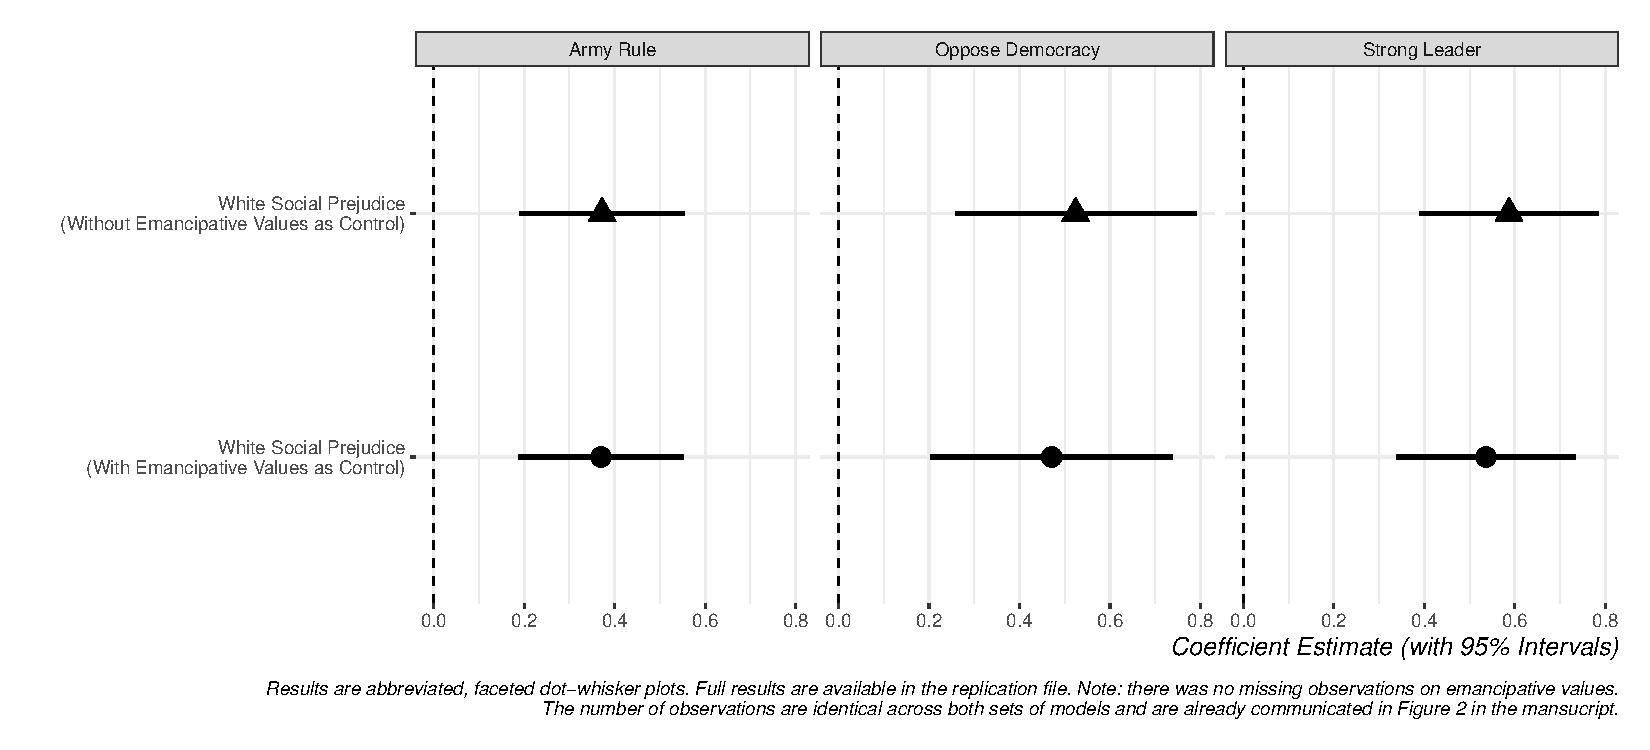
\includegraphics{figs/noemanc.pdf}
\caption{\label{fig:noemanc}Abbreviated Dot-and-Whisker Plots of the
Effect of White Social Prejudice on Anti-Democratic Orientations (with
and without Emancipative Values)}
\end{figure}

Finally, Figure \ref{fig:cai} shows the results of models that drop the
emancipative values variable in favor of the child autonomy index of
interest to the authoritarianism scholarship
\citep[see][]{stenner2005tad}. Whereas the child autonomy index and the
autonomy component of the emancipative values variable are highly
correlated (\emph{r} = .704), this test drops the emancipative values
variable for the child autonomy index. The figure is purposely
abbreviated to highlight just the effect of the child autonomy index and
the white social prejudice measure. The results show a significant and
negative effect of the child autonomy index in just two of the three
models, though the negative sign is consistent with the intuition from
the authoritarianism scholarship. Notice, however, the white social
prejudice measure is unaffected.

\begin{figure}
\centering
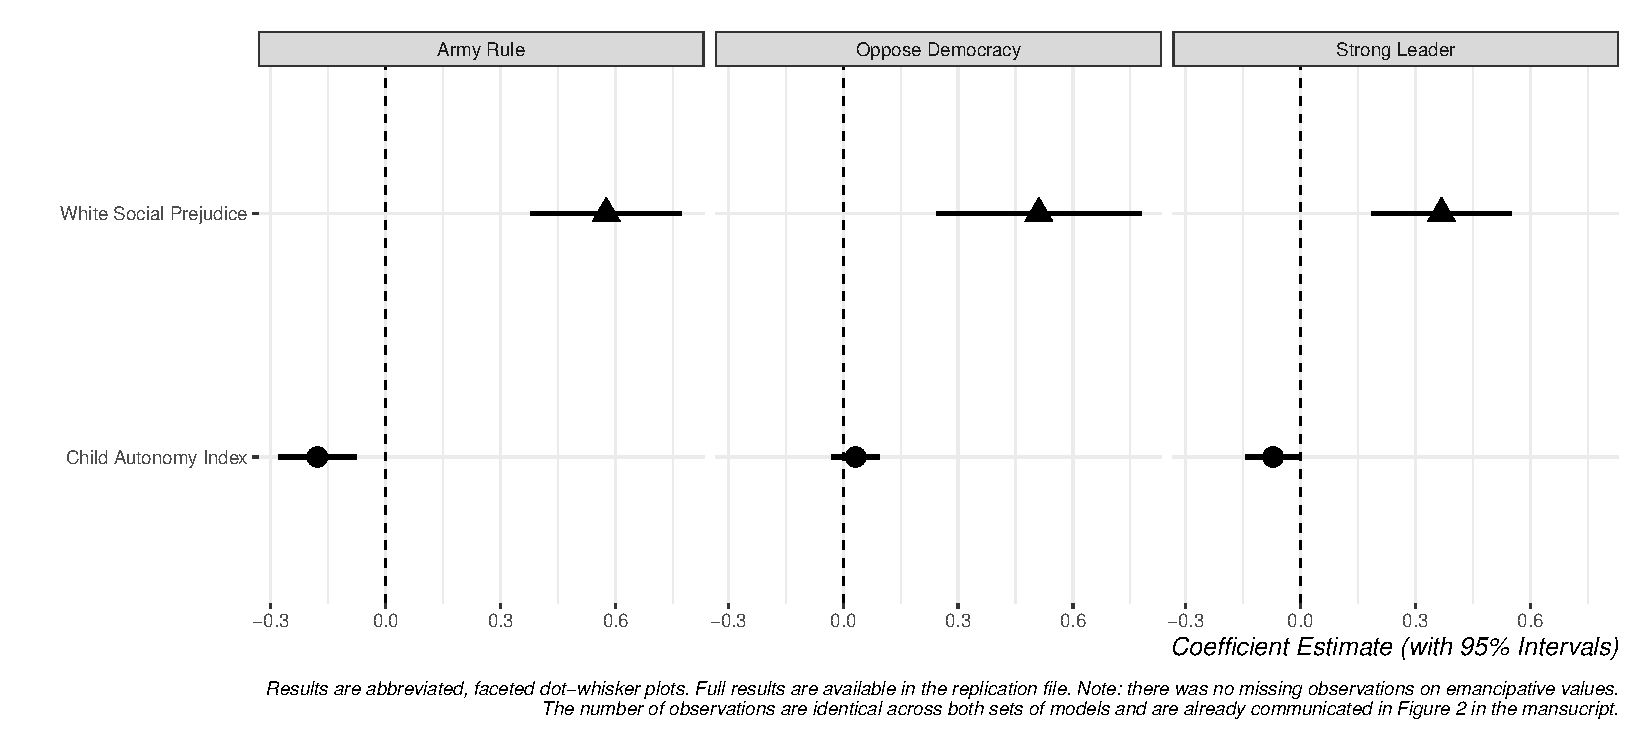
\includegraphics{figs/cai.pdf}
\caption{\label{fig:cai}Abbreviated Dot-and-Whisker Plots of the Effect
of White Social Prejudice on Anti-Democratic Orientations (with Child
Autonomy Index Instead of Emancipative Values)}
\end{figure}





\newpage
\singlespacing 
\bibliography{../refs.bib}

\end{document}
